\documentclass[a4paper, 12pt]{class/thyuthesis}

\title{Approaches to 3-D Shape Recognition and Human Pose Estimation}

\author{Tsz-Ho Yu}
\collegeordept{Darwin College}
\university{\href{http://www.cam.ac.uk}{University of Cambridge}}
\crest{
\includegraphics[width=75mm]{class/CamLogo.pdf}}

\degree{Doctor of Philosophy}
\degreedate{Yet to be decided}

% turn of those nasty overfull and underfull hboxes
\hbadness=10000
\hfuzz=50pt

% 1.5 line spacing
\OnehalfSpacing

\include{00-global-def}

\begin{document}

\maketitle

\setcounter{secnumdepth}{3}
\setcounter{tocdepth}{3}

\frontmatter
\pagenumbering{roman}

\begin{abstracts}
	This is abstract
\end{abstracts}

\begin{acknowledgements}
	This is the acknowledgements.
\end{acknowledgements}


\tableofcontents \newpage
\listoffigures \newpage
\listoftables
%\printnomenclature  %% Print the nomenclature
%\addcontentsline{toc}{chapter}{Nomenclature}

\mainmatter

\part{3-D Shape Recognition}
\include{10-def}
\chapter{Introduction}
This is some test \cite{WeiICCV2009}.

\include{12-relatedwork}
\include{13-detectoreval}
\include{14-3dreg}
\include{15-discussion}

\part{3-D Human Pose Estimation}

%%%%%%%%%%%%%%%%%%%%%%%%%%%%%%%%%
% POSE ESTIMATE
%%%%%%%%%%%%%%%%%%%%%%%%%%%%%%%%%

\newcommand{\snippet}{S}
\newcommand{\snippetlen}{l}
\newcommand{\sframe}{I}
\newcommand{\timenow}{t}

% features 
\newcommand{\fset}{\mathcal{X}}
\newcommand{\feature}{\mathbf{x}}

% action  
\newcommand{\aset}{\mathcal{A}}
\newcommand{\action}{a}

% pose
\newcommand{\pset}{\mathcal{Y}}
\newcommand{\pose}{\mathbf{y}}

% compressed pose 
\newcommand{\ppset}{\mathcal{U}}
\newcommand{\ppose}{\mathbf{u}}

% votes in ADF 
\newcommand{\vset}{V}
\newcommand{\vote}{v}
\newcommand{\nvset}{N_{\vset}}

% final results 
\newcommand{\finalpose}{\Theta}
\newcommand{\finalvariance}{\Lambda}

%% forests and trees 
\newcommand{\forestd}{\mathcal{D}}
\newcommand{\forestr}{\mathcal{R}}
\newcommand{\ntreed}{\mathrm{N_{\forestd}}}
\newcommand{\ntreer}{\mathrm{N_{\forestr}}}
\newcommand{\treed}{\mathbf{d}_d}
\newcommand{\treer}{\mathcal{r}_r}

% snippets
\newcommand{\snippetnow}{\mathcal{\snippet}_{\timenow}}

\newcommand{\posead}{\mathbf{\alpha}}
\newcommand{\posepr}{\mathbf{\beta}}
\newcommand{\posez}{\mathbf{\gamma}}
\newcommand{\rset}{\mathbf{r}}

\newcommand{\realnum}{\mathbb{R}}
\newcommand{\posnum}{\mathbb{Z^{+}}}

\newcommand{\nsnippet}{\mathrm{N_{\snippet}}}
\newcommand{\nframefeature}{\mathrm{N_{\sframe_{\timenow}}}}
\newcommand{\njoints}{\mathrm{N_{J}}}


\newcommand{\nhyp}{\mathrm{N_{h}}}

\newcommand{\treeth}{\tau}

\newcommand{\normdist}{\mathcal{N}}

\newcommand{\infogain}{\mathrm{H_{a}}}
\newcommand{\qualityad}{\mathrm{H}} 
\newcommand{\qualityjr}{\mathrm{H_{p}}} 
\newcommand{\nclass}{C}
\newcommand{\pcadim}{6}

\newcommand{\videoth}{p}
\newcommand{\frameth}{q}
\newcommand{\hypth}{r}

\newcommand{\nodeweight}{\omega}
\newcommand{\termnode}{{\hat{n}}}
\newcommand{\curnode}{n}

%% HAND ESTIMATE 

\newcommand{\viewterm}{Q_{a}}
\newcommand{\classterm}{Q_{p}}
\newcommand{\regterm}{Q_{v}}
\newcommand{\pairterm}{Q_{t}}
\newcommand{\usterm}{Q_{u}}
\newcommand{\tssterm}{Q_{tss}}
\newcommand{\vpjterm}{Q_{apv}}
\newcommand{\qterm}{Q}
\newcommand{\entropy}{H}

\newcommand{\patch}{\mathbf{x}}
\newcommand{\patchset}{\mathcal{X}}
\newcommand{\splitfunc}{\theta} 
\newcommand{\splitfuncset}{\Theta} 
\newcommand{\splitfuncc}{\theta^{*}} 
\newcommand{\viewparam}{\alpha}
\newcommand{\classparam}{\beta}
\newcommand{\regparam}{\gamma}
%\newcommand{\usparam}{\delta}
%\newcommand{\pairparam}{\zeta}
\newcommand{\tssparam}{\omega}

% margin
\newcommand{\margin}{\Delta}

% GMM model
\newcommand{\GMM}{\mathcal{G}}
\newcommand{\testGMM}{\hat{\mathcal{G}}}

%
\newcommand{\nview}{|\viewlabelset|}
\newcommand{\nviewx}{3}
\newcommand{\nviewy}{5}
\newcommand{\nviewz}{9} 

% numbers!
\newcommand{\njoint}{16}
\newcommand{\ntree}{N_{t}}

% data
\newcommand{\totalset}{\mathcal{D}} 
\newcommand{\realset}{\mathcal{R}}
\newcommand{\reallset}{\mathcal{R}_{l}}
\newcommand{\realuset}{\mathcal{R}_{u}}
\newcommand{\synset}{\mathcal{S}} 
%\newcommand{\ctotalset}{\mathcal{D}^{*}} 
%\newcommand{\crealset}{\mathcal{R}^{*}}
%\newcommand{\creallset}{\mathcal{R}^{*}_{l}}
%\newcommand{\crealuset}{\mathcal{R}^{*}_{u}}
%\newcommand{\csynset}{\mathcal{S}^{*}}
\newcommand{\ctotalset}{\mathcal{D}} 
\newcommand{\crealset}{\mathcal{R}}
\newcommand{\creallset}{\mathcal{R}_{l}}
\newcommand{\crealuset}{\mathcal{R}_{u}}
\newcommand{\csynset}{\mathcal{S}}
\newcommand{\clset}{\mathcal{L}}
\newcommand{\viewlabel}{\mathbf{a}}
\newcommand{\jointlabel}{p}
\newcommand{\votelabel}{\mathbf{v}}
\newcommand{\houghvote}{\mathbf{\nu}}
\newcommand{\joint}{\mathbf{j}}
\newcommand{\viewlabelset}{\mathcal{A}}
\newcommand{\jointlabelset}{\mathcal{P}}
\newcommand{\votelabelset}{\mathcal{J}}
\newcommand{\real}{r}
\newcommand{\syn}{s} 

\newcommand{\ksynset}{\mathcal{K}}
% determinant
\newcommand{\trvar}{\mathrm{\Lambda}}
\newcommand{\trace}{\mathrm{trace}}

% kinematic prior
% \newcommand{\kprior}{\mathrm{K}}
\newcommand{\ngmm}{N}
\newcommand{\onegmm}{n}

% association functions? 
\newcommand{\assoc}{\mathrm{\Psi}}

% naming 
\newcommand{\STR}{STR} 
\newcommand{\STRF}{STRF}

% Testing stage
\newcommand{\testimg}{\mathbf{I}} 
\newcommand{\testpatchset}{\hat{\patchset}}
\newcommand{\testpatch}{\hat{\patch}}
\newcommand{\testviewlabel}{\hat{\viewlabel}}
\newcommand{\testjointlabel}{\hat{\jointlabel}}
\newcommand{\testvotelabel}{\hat{\votelabel}}
%\newcommand{\testviewlabel}{\hat{\viewlabel}}
%\newcommand{\testjointlabel}{\hat{\jointlabel}}
\newcommand{\testjoint}{\mathbf{Y}}
\newcommand{\testonejoint}{\mathbf{y}}
\newcommand{\testjointset}{\mathcal{Y}}
%\newcommand{\testoccthres}{t_{occ}}
\newcommand{\testqualthres}{t_{q}}
\newcommand{\testoccset}{\mathcal{O}}

% dataset number
\newcommand{\nreal}{1000}
\newcommand{\nsynperview}{2500}
\newcommand{\nsyn}{2500}
\newcommand{\nlreal}{200}

\include{21-intro}
\include{22-relatedwork}
\chapter{Action Recognition}
\section{Introduction}
\label{sec:actreg:intro}

Recognising human actions from videos has been widely studied for practical applications such as human-computer interfaces, digital entertainment, visual surveillance and automatic video indexing. Despite popularity of the topic in computer vision research, some issues still remain unsolved for realising its potentials:
\begin{itemize}

\item While \emph{time efficiency} is of vital importance in real-world action recognition systems, current methods seldom take the computational complexity into full consideration. State-of-the-art algorithms have reported satisfactory accuracies on standard human action data sets. They, however, utilise complex algorithms to improve accuracies at the expense of increasing overall computational time.

\item Action classification with \emph{a short response time} is beneficial to continuous recognition in human-computer interaction. Typically, an class label is assigned after the entire query video is analysed, or a large lookahead is required to collect sufficient features. In fact, as suggested by \cite{Schindler2008}, actions can be recognised from very short sequences called the ``snippets''.

\item {\em Structural information} is a useful cue for action recognition. A standard ``bag of words'' model has proven effective for action recognition owing to its rich description power of local appearance information and its inherent benefits to cope with scale changes, translation and cluttered backgrounds. It, however, does not consider structural relationship among features. 

\end{itemize}

Addressing the aforementioned challenges, we present a novel method for human action recognition.
The goal of this work is to design a very fast but equally effective action recogniser.
In the method we intend to exploit as much information as possible in a relatively short video sequence, local appearance and structural information are integrated adaptively.
The major contributions include the followings.

Firstly, inspired by the work of Shotton \etal{Shotton2008}, we extend the use of semantic texton forests from 2D image segmentation to spatiotemporal analysis. STFs are ensembles of random decision trees that translate interest points into visual codewords. In our method, STF performs directly on video pixels without computing expensive local descriptors and efficiently generates codewords. As well as being faster than a traditional flat codebook such as k-means clustering, STF achieves high effectiveness comparable to that of existing approaches.
As far as we are aware, this is the first method that uses STF in action recognition studies.

Secondly, the method combines structure and local appearance information based on STF. This results into a richer description of human actions, hence actions can be classified in very short video sequences. Building on the work of Ryoo and Aggarwal{Ryoo2009}, we introduce the multi-pyramidal spatiotemporal relationship match (MpSRM). In the original approach, structural information of spatiotemporal features are matched linearly. Quantization errors affect the robustness of recognition results. Taking the inherent benefit of the hierarchical structure of semantic texture forest, a pyramidal match kernel \cite{Grauman2005} is employed to alleviate the quantization problem.
A fast and effective classifier, namely k-means forest classifier, is also proposed.

Lastly, several techniques are employed to improve the recognition speed and accuracy. A novel spatiotemporal interest point detector, called V-FAST, is designed based on the FAST 2D corners{Rosten2006}. The recognition accuracy is improved by adaptively combining MpSRM and the bag of semantic texton (BOST) method \cite{Shotton2008}.

The rest of the paper is structured as follows: In section \ref{sec:relatedwork}, related work are reviewed and, in section \ref{sec:overview}-\ref{sec:combine}, the proposed methods are detailed. Evaluation results are reported and discussed in Section \ref{sec:experiments} and the conclusion is drawn in Section \ref{sec:discussion}.


\section{Related Work}
\label{sec:relatedwork}
State-of-the-art action recognition methods have shown the effectiveness of local appearance-based features, as a ``bag of words'' model is especially popular in the literature \cite{Dollar2005, Riemenschneider2009, Niebles2008, Schuldt2004, Wong2007}. A codebook is learned to quantise input features into visual codewords. Classification is then performed on histograms of codewords. Generally, a large codebook is required to obtain a high recognition accuracy, yet an oversized codebook leads to high quantisation errors and overfitting. K-means clustering is a widely adopted algorithm in codebook learning. Feature quantization by a large flat codebook such as k-means is, however, computationally heavy. Therefore, tree-based codebooks have been studied to increase the efficiency of feature quantisation. 
%Since Moosmann \etal{MoosmannNIPS2006}, random forest has been increasingly popular as a powerful discriminative codebook in many tasks e.g. image classification and segmentation \cite{shottonCVPR2008}, owing to its good generalisation and speed. 
Since Moosmann \etal \cite{Moosmann2007}, random forests have been increasingly used in many tasks \eg image classification and segmentation \cite{Shotton2008}, owing to its good generalisation and efficiency. Similarly, Oshin \etal \cite{Oshin2009} recognise actions by analysing the distribution of interest points by random ferns. Lin \etal \cite{Lin2009} used a prototype tree to encode holistic motion-shapes descriptors. Mikolajczyk and Uemura \cite{Mikolajczyk2008} build clustering trees from the centroids computed from k-means algorithm. 
%Using a tree structure makes the quantisation process efficient, however, expensive features and classifier used in{linICCV2009,mikolajczykCVPR2008} make the overall process still heavy.
Hierarchical codebooks enable fast feature quantisations, but the expensive features and classifiers used in{Lin2009,Mikolajczyk2008} make the overall processes still heavy.

Standard bag of words models contain only local appearance information. While structural context could be useful in describing some action classes, it is often omitted in current action recognition methods.
On the other hand, some studies{Gorelick2007, Fathi2008, Lin2009, Kim2007} have implied that structural or holistic features can be as effective as local features.
Several recent studies have attempted to augment structural information into local appearance features. Scovanner \etal \cite{Scovanner2007} employ a two-dimensional histogram to describe the feature co-occurrences. Savarese \etal \cite{Savarese2008} propose ``correlograms'' to measure the similarity of actions globally. Wong \etal \cite{Wong2007} present the pLSA-ISM model, which is an extension of a probabilistic model pLSA with augmented spatial information. 
Tran and Sorokin \cite{Tran2008} and Zhang \etal \cite{Zhang2008} capture structural information directly by using a global shape descriptor.
Since these methods \cite{Wong2007,Tran2008, Zhang2008} encode the hosllistic structures with respect to a reference position \eg a center of ROI (region of interests), they require manual segmentation and computationally-demanding detection of ROI in training and testing respectively. 
However, the structural relationship between among individual features are not fully utilised in these techniques.
Most recently, Ryoo and Aggarwal{Ryoo2009} propose the spatiotemporal relationship match (SRM) which represents structures by a set of pairwise spatiotemporal association rules. Kovashka and Grauman \cite{Kovashka2010} exploit structural information by learning an optimal neighbourhood measure on interest points. Despite of the high accuracies reported, speed and quantisation error are the major issues because flat k-means codebooks are used.

The pyramid match kernel (PMK){Grauman2005} is widely used in recent image-based object detection and matching studies. PMK exploits multi-resolution histograms. Similar points that do not match at fine resolutions have the chance to match at lower resolutions. Hence, PMK reduces quantisation errors and enhances robustness. Liu and Shah \cite{Liu2008} matched interest points in multiple resolutions using PMK and reported improved results, however the features are only matched spatially but not semantically.

Design of interest point detector/descriptor and classifiers also plays an essential role. 
%Just to name a few, Laptev and Lindeberg{laptevICCV2003} and Dollar \etal \cite{dollarPETS2005} propose interest points detector which are the extensions of 2D Harris corners. These interest point detector are widely adopted in existing approaches.
Just to name a few, the detectors designed by Laptev and \cite{Laptev2005} and Dollar \etal \cite{Dollar2005} are commonly adopted in most existing methods. Both of them are the extensions of the two-dimensional Harris corner.
Wong and Cipolla{Wong2007a} extract interest points using global information.
Oikonomopoulos \etal{Oikonomopoulos2005} compute spatiotemporal saliency by measuring the entropy within a spherical neighbourhood.
To describe interest points, histogram of gradients (HOG) and optical flow are popular among earlier approaches \cite{Dollar2005, Niebles2008, Schuldt2004}. Scovanner \etal \cite{Scovanner2007} proposed a three-dimensional version of Lowe's popular SIFT descriptor \cite{Lowe2004}. Willems \etal \cite{Willems2009} used an extended SURF descriptor for action recognition.
Some common classifiers used in action recognition include K-NN classifiers, support vector machines and boosting, which are complex to attain a sufficient real-time performance.

With increasing interests in practical applications, real-time action recognition algorithms have attracted new attentions. For instance, Yeffet and Wolf \cite{Yeffet2009} utilise dense local trinary patterns with a linear SVM classifier. Gilbert \etal \cite{Gilbert2009} propose a fast multi-action recognition algorithm by finding reoccurring patterns on dense 2D Harris corners by a data-mining algorithm.
Patron-Perez and Reid \cite{Patron2007} designed a probabilistic classifier that recognise actions continuously with a sliding window. 
Bregonzio \etal \cite{Bregonzio2009} consider actions as clouds of points, efficient classification is done by analysing histogram of point clusters. Although real-time performances have been reported by these methods, their computation bottlenecks in visual codebook have not yet addressed. 
Some methods require a prior segmentation or a long sequence for classification, rendering these methods efficient but not responsive. 

\section{Overview of the proposed method}
\label{sec:overview}
An overview of the proposed approach is illustrated in figure \ref{img:flow}. Spaiotemporal interest points are first localised by the proposed V-FAST detector. Visual codewords are generated from the interest points by a semantic texton forest. Using pairwise codewords and their spatiotemporal associations, histograms that capture both local-appearance and structural information are constructed. Classification is performed efficiently using a hierarchical k-means algorithm with pyramid match kernels. The proposed method is adaptively combined with the prior-art that uses the bag of semantic texton (BOST) and random forest classifier to further improve the recognition accuracy.
The proposed recognition framework is flexible. Depending on the application, simple spatiotemporal volumes can be replaced by other local features, such as HOG or tracked trajectories.

\begin{figure}
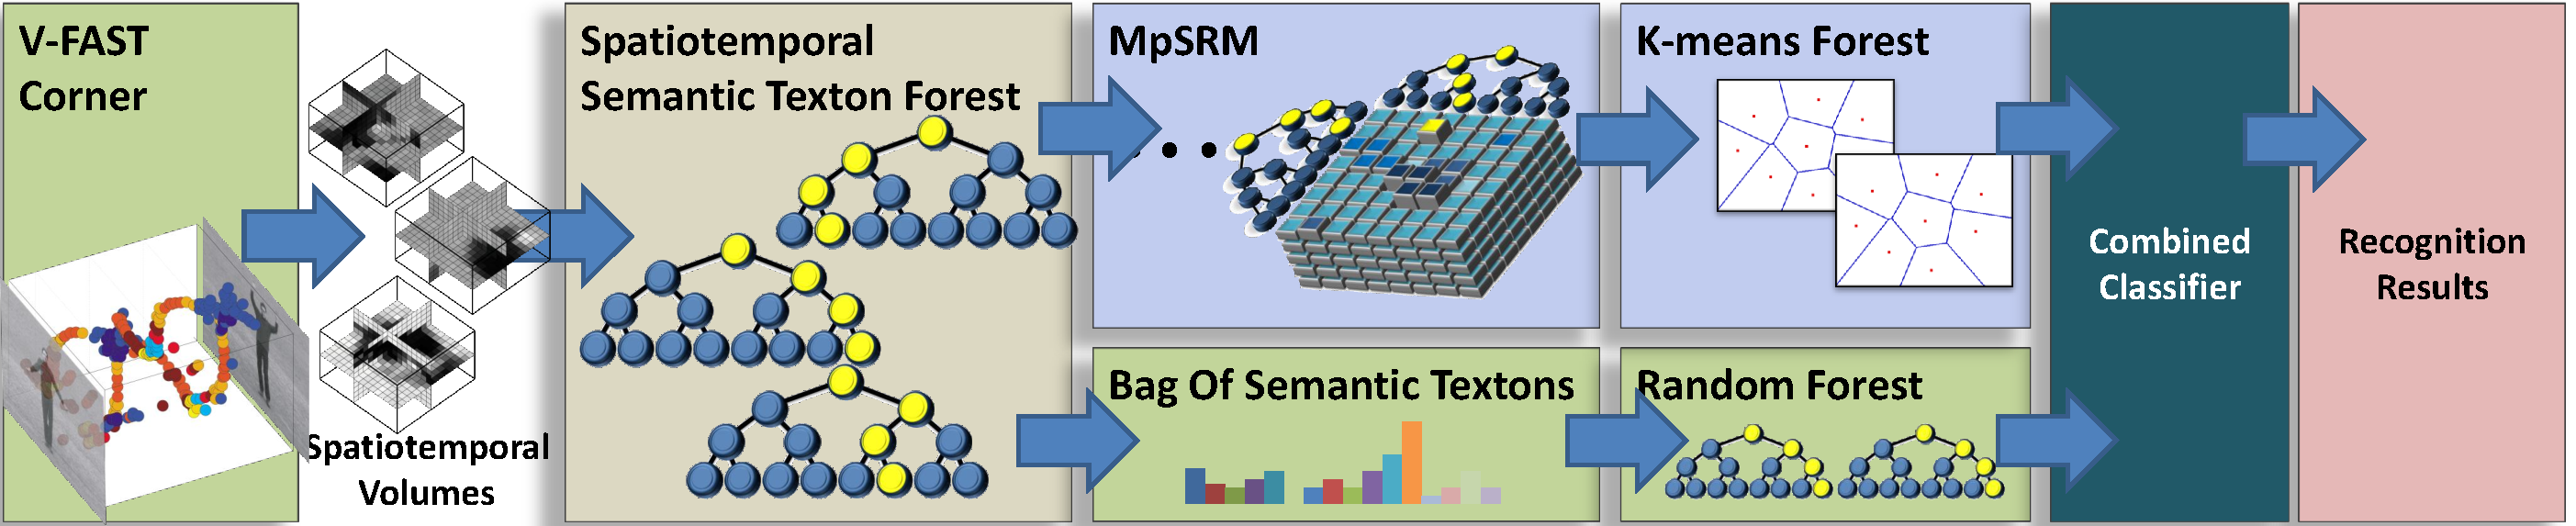
\includegraphics[width=1.0\linewidth]{fig/actreg/fig1_new.pdf}%flow.png}
\caption{Overview of the proposed approach}
\label{img:flow}
\end{figure}

\section{V-FAST Interest Point Detector}
\label{sec:fastest}
The V-FAST (Video FAST) interest point is an extended version of the two-dimensional FAST corner \cite{Rosten2006} to the spatiotemporal domain. It considers pixels in three orthogonal Bresenham circles with radius $r$ on $XY$, $YT$ and $XT$ planes. Similar to FAST, saliency is detected on a plane if there exists $n$ contiguous pixels on the circle which are all brighter than a reference pixel $p(x,y,t)$ plus a threshold $t$, or all darker than $p(x,y,t)-t$. An interest point is detected when the reference pixel shows both spatial ($XY$-plane) and temporal ($XT$-plane or $YT$-plane) saliency. The V-FAST detector gives a denser set of interest points, which enables accurate classification from relatively short sequences. Figure \ref{img:fastest} illustrates how interest points are detected using a 42-pixel V-FAST interest point detector with $r = 3$.
\vspace{-2mm}
\begin{figure}[h]
\centering
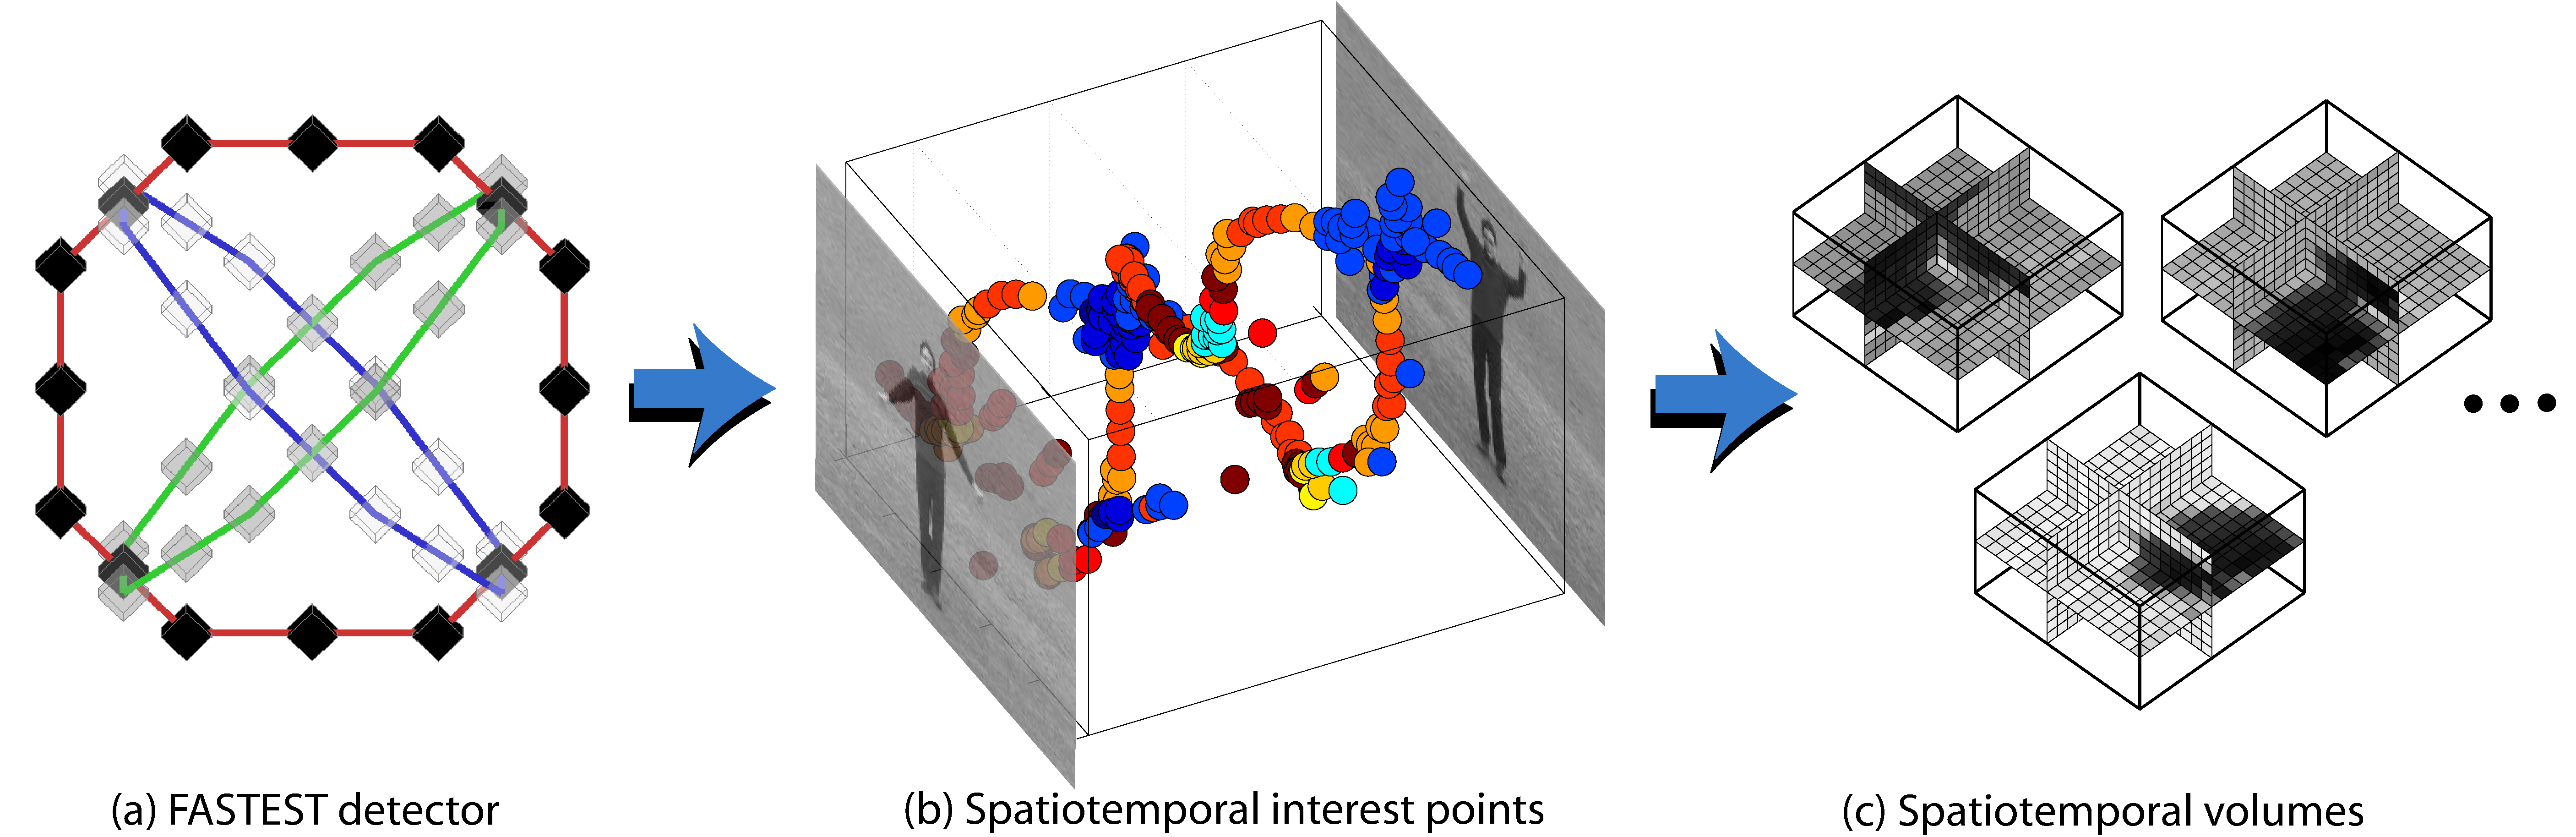
\includegraphics[width=0.8\linewidth]{fig/actreg/fig2_tot.pdf}%fastest.png}
\caption{Spatiotemporal interest points localised by the proposed V-FAST detector}
\label{img:fastest}
\end{figure}\vspace{-5mm}

\section{Spatiotemporal Semantic Texton Forest}
\label{sec:stf}
The semantic texton forest{Shotton2008} is an ensemble of randomised decision trees which textonise input video patches into semantic textons. It is extremely fast to evaluate, since only a small number of simple features is used to traverse the trees. It is also a powerful discriminative codebook composed of multiple decision trees. Figure \ref{img:stf} illustrates how visual codewords are generated using the spatiotemporal semantic texton forest in the proposed method. It acts on small spatiotemporal volumes $p(x,y,t)$, which are localised around the detected interest points from input videos. The training process of STF is similar to that of random forest. At each split node, a number of candidate split functions are generated randomly, the one that maximises the information gain is chosen. The split functions in this work are defined as the weighted differences of two pixels from the input space-time patches: 
\begin{equation}
\mathit{f}(p) = w_1 \cdot p(x_1,y_2,t_1) - w_2 \cdot p(x_2,y_2,t_2) > threshold
\end{equation}
Features are passed down the $M$ trees. Hence, a STF codebook has a size of $L=\sum_m^M L_m$  where $L_m$ represents the number of leaf nodes i.e. codewords in $m$-th tree. Figure \ref{img:stf} (right) shows the two codewords generated with respect to the example split function.
\begin{figure}
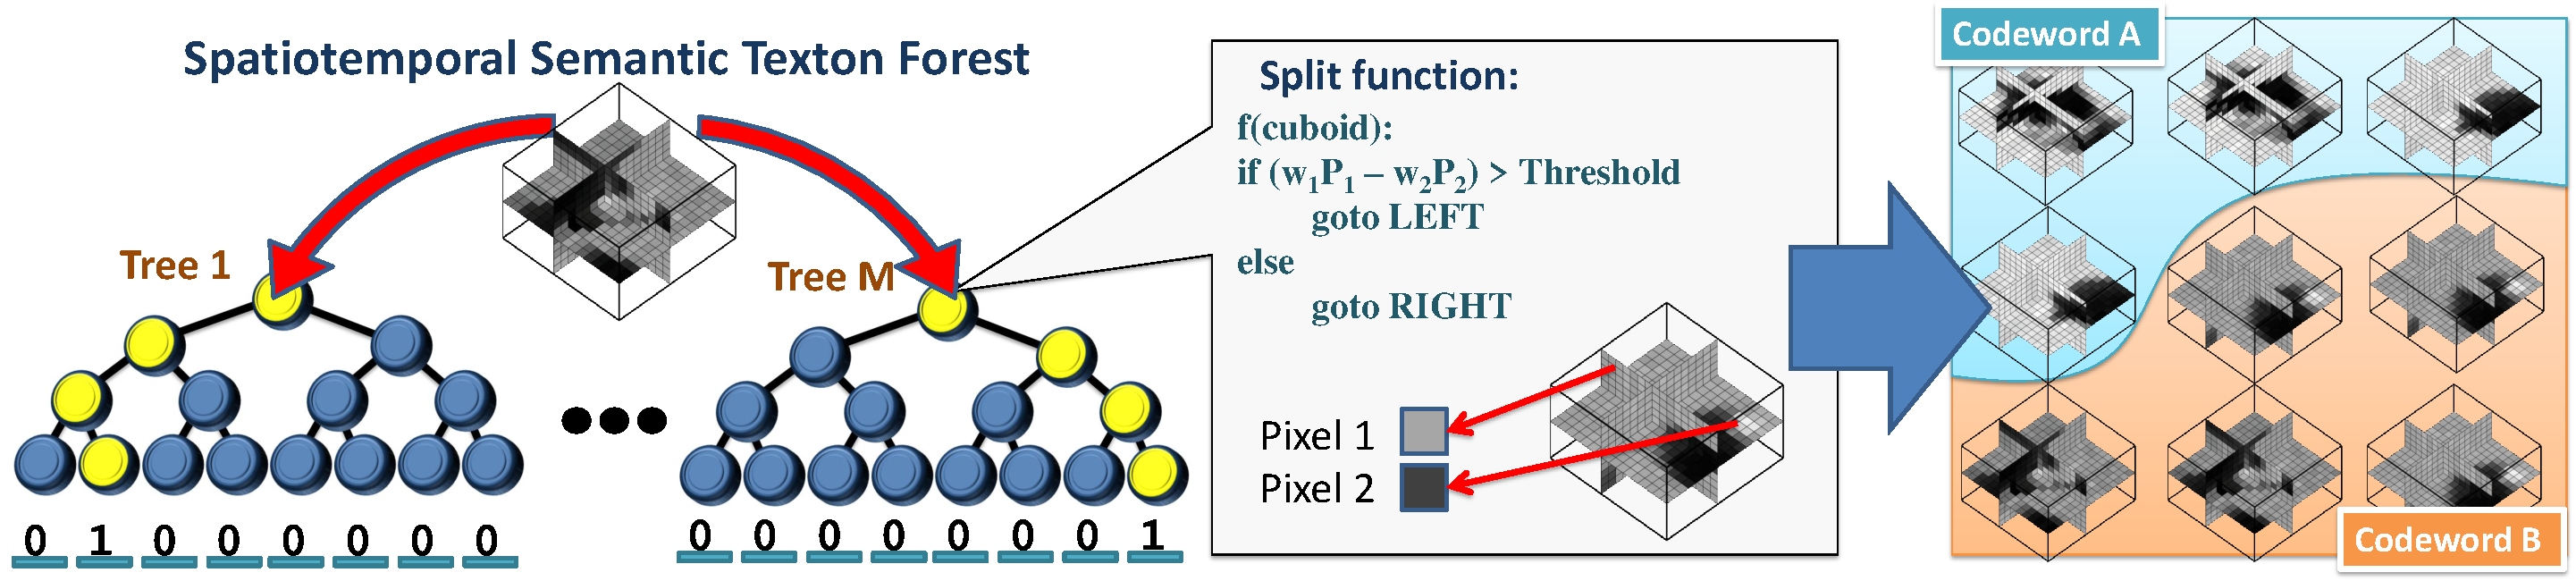
\includegraphics[width=1\linewidth]{fig/actreg/stf.pdf}%stf.png}
\caption{Visual codeword generation by Spatiotemporal Semantic Texton Forest}
\label{img:stf}
\end{figure}
Table \ref{tab:codebook} summarises a comparison between STF and k-means algorithms.
\begin{table}
\begin{center}
{\footnotesize
\begin{tabular}{|c|c|c|c|}
\hline
\textbf{ Algorithm} & \textbf{ Copmlexity} & \textbf{ Relative Speed}* & \textbf{ Hierarchical} \\
\hline
\hline
k-means & $O(K)$ & $1$ & no \\
Hierarchical k-means & $O(b\log_{b}(K))$ & $43.51$ & yes \\
{\color{blue}{STF}} & {\color{blue}{ $ O(\log_{2}(K)) $ }} & {\color{blue}{$559.86$}} & {\color{blue}{yes}}\\
\hline
\multicolumn{4}{p{0.75\linewidth}}{\scriptsize Relative speed is measured by computing $1$ million feature vectors with $405$ dimensions. Size of codebook $K$ is $1905$. The branching factor $b$ for k-means algorithm is $16$.}
\end{tabular}
}
\end{center}
\caption{Comparison of semantic texton forest and k-means codebooks.}
\label{tab:codebook}
\end{table}

\section{Multi-pyramidal Spatiotemporal Relationship Match}
\label{sec: MpSRM}
Multi-pyramidal spatiotemporal relationship match (MpSRM) is presented to encapsulate both local-appearance and structural information efficiently. Semantic texton forest quantises local space-time volumes into codewords in multiple texton trees. For each tree, a three-dimensional histogram is constructed by analysing pairs of codewords and their structural relations (see figure~\ref{img:mpsrm} (left and middle)). For each histogram, a novel pyramid match kernel is proposed for robust matching (figure~\ref{img:mpsrm} (right)). Multiple pyramidal matches are then combined to classify a query video. Whereas the spatiotemporal relationship match (SRM){Ryoo2009} relies on a single flat k-means codebook, MpSRM utilises multiple tree codebooks and pyramid match kernels. Its hierarchical structure offers a time-efficient way to perform pyramid match kernel for semantic codeword matching \cite{Grauman2005}.\vspace{-3mm}
\paragraph{Spatiotemporal relationship histograms.}
\begin{figure}
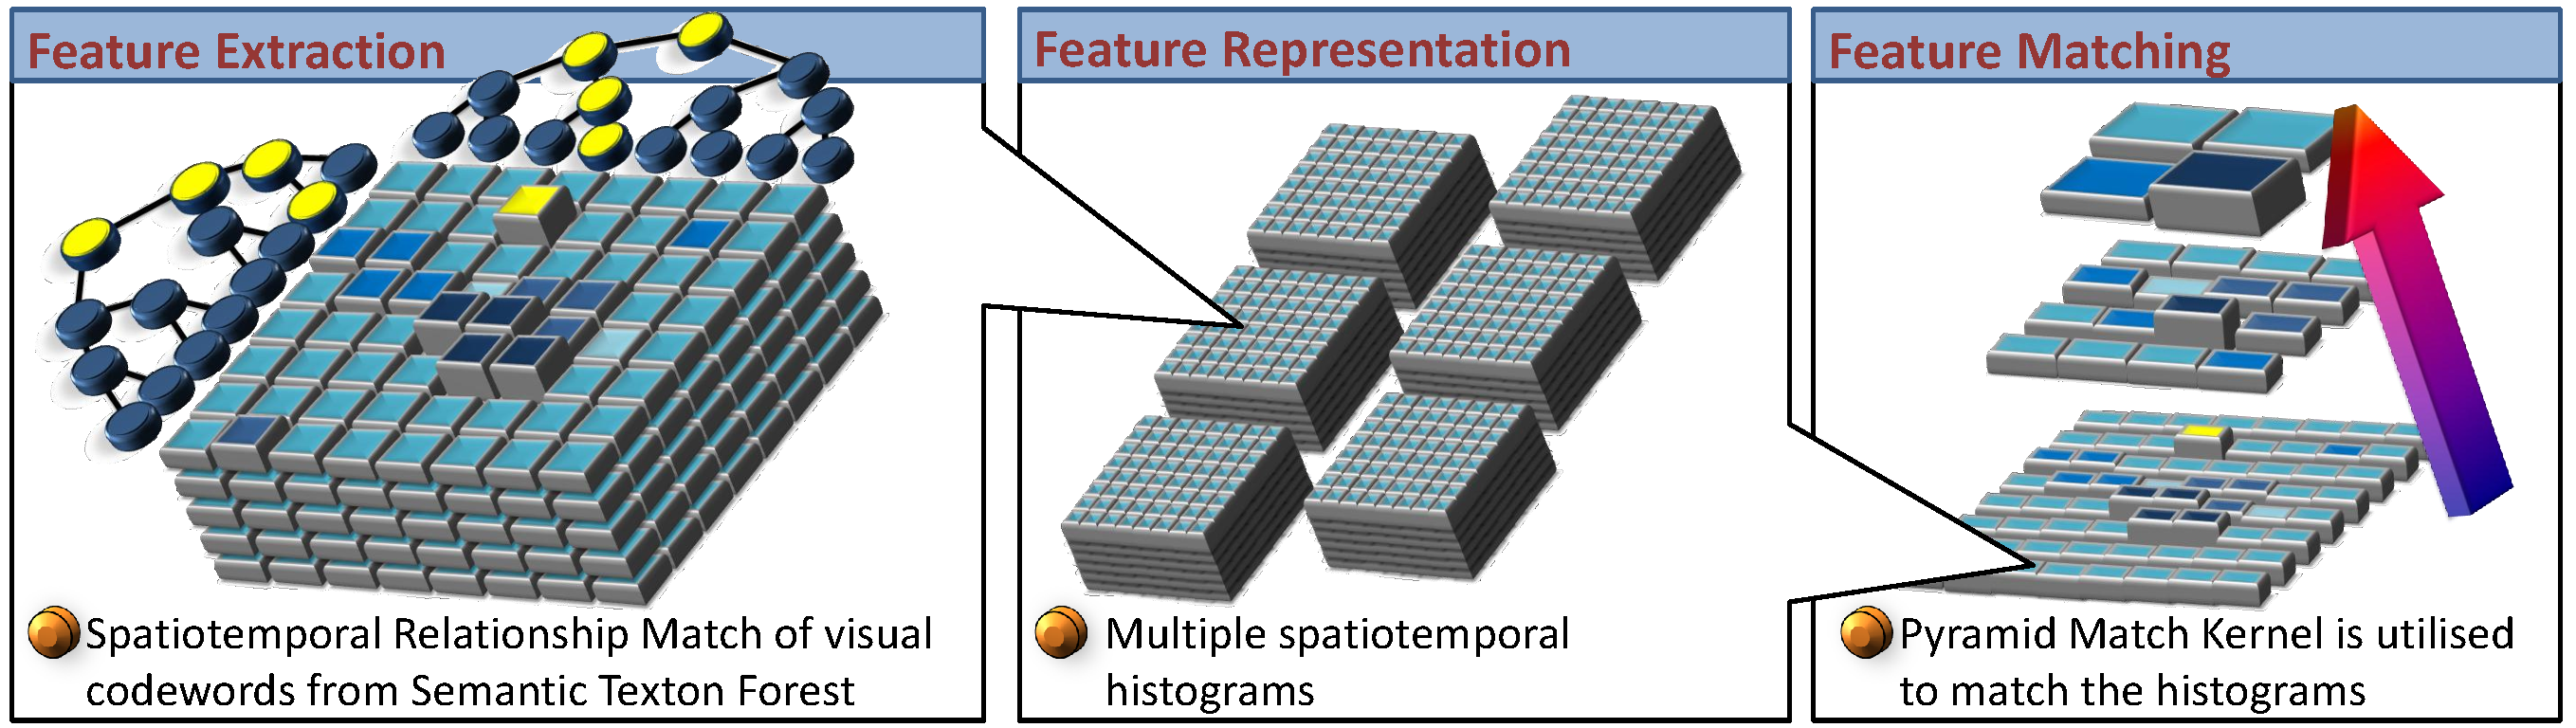
\includegraphics[width=1\linewidth]{fig/actreg/fig4.pdf}%mpsrm.png}
\caption{Multi-pyramidal spatiotemporal relationship match (MpSRM)}
\label{img:mpsrm}
\end{figure}

Short video sequences are sequentially sampled from an input video in very short intervals (\eg$10$ frames). A set of spatiotemporal interest points $\mathrm{U} = \{u_{i}\}$ are localised. The trained STF assigns visual codewords to the interest points. Therefore, an encoded interest point can be described as $u_{i} = \{x_i, y_i, t_i, l_{m,i}\}, m=1,...,M$, where $x_i, y_i, z_i$ represents a $XYT$-location of the feature and $l_{m,i}$ is the visual codeword i.e. leaf node assigned to $u_{i}$ by the $m$-th tree. A set of pair-wise spatiotemporal associations are designed to capture the structural relations among interest points. By analysing all possible pairs $u_i$ and $u_j$ in $\mathrm{U}$, space-time correlations are described by the following seven association rules $\mathrm{R} = \{ R_1,\dots,R_7\}$:

\begin{align*}%\quad ~~~
& R_{1} ~{\color{blue}overlap}: |t_i - t_j| < \mathrm{T_{o}},   & & R_{4}~{\color{blue}nearXY}: (|x_i - x_j| < \mathrm{T_{n}}) \wedge (|y_i - y_j| < \mathrm{T_{n}}) \nonumber\\
& R_{2} ~{\color{blue}before}: \mathrm{T_{o}} < t_j - t_i < \mathrm{T_{b}}, & & R_{5}~{\color{blue}nearX}: (|x_i - x_j| < \mathrm{T_{n}}) \wedge \sim(nearXY)\nonumber\\
& R_{3} ~{\color{blue}after}: \mathrm{T_{o}} < t_i - t_j < \mathrm{T_{a}}, & & R_{6}~{\color{blue}nearY}: (|y_i - y_j| < \mathrm{T_{n}}) \wedge \sim(nearXY)\nonumber\\
& R_{7} ~{\color{blue}far}: (|x_i - x_j| < \mathrm{T_{f}}) \wedge (|y_i - y_j| < \mathrm{T_{f}}) & \wedge & \sim(nearXY \vee nearX \vee nearY)
\vspace{-3mm}
\end{align*}

Figure \ref{img:mpsrm} illustrates how relationship histograms are constructed and matched in MpSRM. A set of 3D relationship histograms $\{ \mathrm{H}_1(\mathrm{U}),\dots,\mathrm{H}_{M}(\mathrm{U})\}$ are constructed by analysing the pairs of feature points in $\mathrm{U}$. The bin $\mathrm{h}_{m}(i,j,k)$ for the $m$-th tree $\mathrm{H}_{m}(\mathrm{U})$ corresponds to the number of matching $(l_{m,i},l_{m,j})$ codeword pairs by an association $R_k$. The total number of bins in $\mathrm{H}_m(\mathrm{U})$ is $L_m \times L_m \times |\mathrm{R}|$. Despite the enormous size of the relationship histograms, operations on these histograms can be greatly accelerated by using sparse matrices.

\paragraph{Pyramid match kernel for MpSRM.}
Multi-resolution matching of input features is realised by pyramid match kernel (PMK){Grauman2005}. It measures the similarity of two set of features in a multi-resolution histogram space.
The similarity between two sets of interest points $\mathrm{U}$ and $\mathrm{V}$ is measured by pyramid match kernel (PMK) from a multi-resolution histogram space for each tree. At a specific resolution $q$, the two sets $\mathrm{U}$ and $\mathrm{V}$ having the histogram bins $\mathrm{h}^q_{m}(i,j,k)$ and $\mathrm{g}^q_{m}(i,j,k)$ respectively, are matched by histogram intersection in (\ref{eq:hik}). New quantisation levels in the histogram pyramid are formed by increasing bin size. In the proposed method, adjacent bins that share the same parent node in the tree are conveniently merged in (\ref{eq:merge}), creating a new quantisation level $\mathrm{h}^{q+1}_m(i,j,k)$ (the same for $\mathrm{g}^{q+1}_m(i,j,k)$). The match kernel $\mathrm{K}_m$ for MpSRM at the $m$-th tree is then defined in (\ref{eq:pmk}) by the weighted summation of difference between successive histogram intersections. Matches in finer bins score higher similarity than matches in coarser levels by a factor of $\frac{1}{4^{q-1}}$.
\begin{eqnarray}
\label{eq:hik}
\mathrm{I}^q(\mathrm{U},\mathrm{V}) &= & \Sigma_{i=1}^{L_m}\Sigma_{j=1}^{L_m}\Sigma_{k=1}^{7} \left( \min(\mathrm{h}^{q}_m(i,j,k), \mathrm{g}^{q}_m(i,j,k)) \right)\\
\label{eq:merge}
\mathrm{h}^{q+1}_m(i,j,k) &= &\Sigma_{u=1}^{2}\Sigma_{v=1}^{2} \left( \mathrm{h}^{q}_m(2(i-1)+u,2(j-1)+v,k) \right)\\
%\label{eq:newcount}
%D^{q}_m(U,V) &= & I^q_m(U,V) - I^{q-1}_m(U,V) \\
\label{eq:pmk}
\mathrm{K}_m(\mathrm{U},\mathrm{V}) &= & \Sigma_{q = 1}^{Q}\frac{1}{4^{q-1}} \left( \mathrm{I}^{q+1}(\mathrm{U},\mathrm{V}) - \mathrm{I}^{q}(\mathrm{U},\mathrm{V}) \right)
\end{eqnarray}

\paragraph{Kenrel k-means forest classifier.}
The MpSRM is utilised to form the k-means forest classifier. Given a set of training video data $\mathrm{U}_i$, $M$ independent clustering trees are trained by recursively performing k-means algorithm on the pyramid matches. For the $m$-th tree in STF, the hierarchical k-means algorithm aims to partition the training data into $\mathbf{S}=\{S_i\}$, $i=1,...,N$ clusters so as to maximise the intra-cluster similarity by (\ref{eq:kmeans}):
\begin{equation}
\arg\max_{\mathbf{S}} \Sigma_{i = 1}^{N}\Sigma_{\mathrm{U}_j \in S_{i}} \mathrm{K}_m(\mathrm{U}_j, \mu_{m,i})
\label{eq:kmeans}
\end{equation}
where $\mu_{m,i}$ is the centroid of $i$-th cluster. In the testing stage, MpSRM is performed on a query video $\mathrm{V}$ against all centroids $\mu_{m,i}$ at the same level. The query video proceeds to the node with highest similarity score and MpSRM is performed recursively until a left node is reached. Classification is performed by the posterior probability by averaging the class distributions of the assigned leaf nodes $\{ \hat{\mu}_m \}, m=1,...,M$ trees as
\begin{equation}
\arg\max_{c}\mathrm{P}_{H}(c|\mathrm{V}) = \frac{1}{M}\Sigma_{m=1}^{M}\mathrm{P}_{H}(c|\hat{\mu}_{m})
\end{equation}

\section{Combined Classification with BOST}
\label{sec:combine}

\paragraph{Bag of semantic textons.}
The method called bag of semantic textons (BOST) developed for image classification{Shotton2008} is applied to analyse local space-time appearance. A 1-D histogram $\mathrm{B}$ is obtained by counting the occurrences of interest points at every node in the STF codebook, hence histogram size $|\mathrm{B}|$ is the total number nodes in the STF. Since its dimension $L$ is relatively low (c.f. the MpSRM histogram has $L_m \times L_m \times |\mathrm{R}|$ dimension), standard random forest \cite{Breiman2001} is applicable as a fast and powerful discriminative classifier, which has proved powerful in image categorisation and visual tracking. The random forest trained on the BOST histograms classifies a query video $\mathrm{V}$ by the posterior probability by averaging the class distributions over the assigned leaf nodes $\{\hat{l}_1,\dots,\hat{l}_{m}\}, m=1,...M$ trees in the STF: $\mathrm{P}_{B}(c|V) = \frac{1}{M}\sum_{m=1}^{M}\mathrm{P}_{B}(c|\hat{l}_m)$.

\paragraph{Combined classification.} The task of action recognition is performed separately by the proposed kernel k-means forest classifier and by the BOST method. While MpSRM has proved effective in most of the cases owing to its both local and structural information, BOST works well owing to its powerful RF classifier on some particular action classes. By integrating classification results of both methods, average performance is significantly improved. Final class label is assigned to the class $c$ which obtains the highest combined posterior probability as
\begin{equation}
\arg\max_{c}\mathrm{P}(c|\mathrm{V}) = \alpha_c \mathrm{P}_{H}(c|\mathrm{V}) + (1 - \alpha_c) P_{B}(c|\mathrm{V})
\label{eq:combine}
\end{equation}
where the weight $\alpha_c$ is selected to maximise the true positive ratio (sensitivity) of a particular class $c \in C$. Values of $\alpha_c$ are computed using gradient descent or simple line search.

\section{Experiments}
\label{sec:experiments}
The proposed method was tested on the well-known KTH data set \cite{Schuldt2004} and the UT-interaction data \cite{Ryoo2010}, a more challenging set \cite{Ryoo2009}. Other published state-of-the-art approaches are compared with the proposed method in terms of recognition accuracy. Computational time of our method is also reported. The experimental prototype was implemented in C++ on a standard PC. The system runs in real-time and makes decisions in a continuous manner (see the supplementary video submitted). 
%%%%%%%%%%%%%%%%%%%%%%%%%%%%%%%%%%%%%%%%%%%%%%%%%%%%%%%%%%%
% Example frames of KTH and UT-interaction
%%%%%%%%%%%%%%%%%%%%%%%%%%%%%%%%%%%%%%%%%%%%%%%%%%%%%%%%%%%
\begin{figure}
\centering
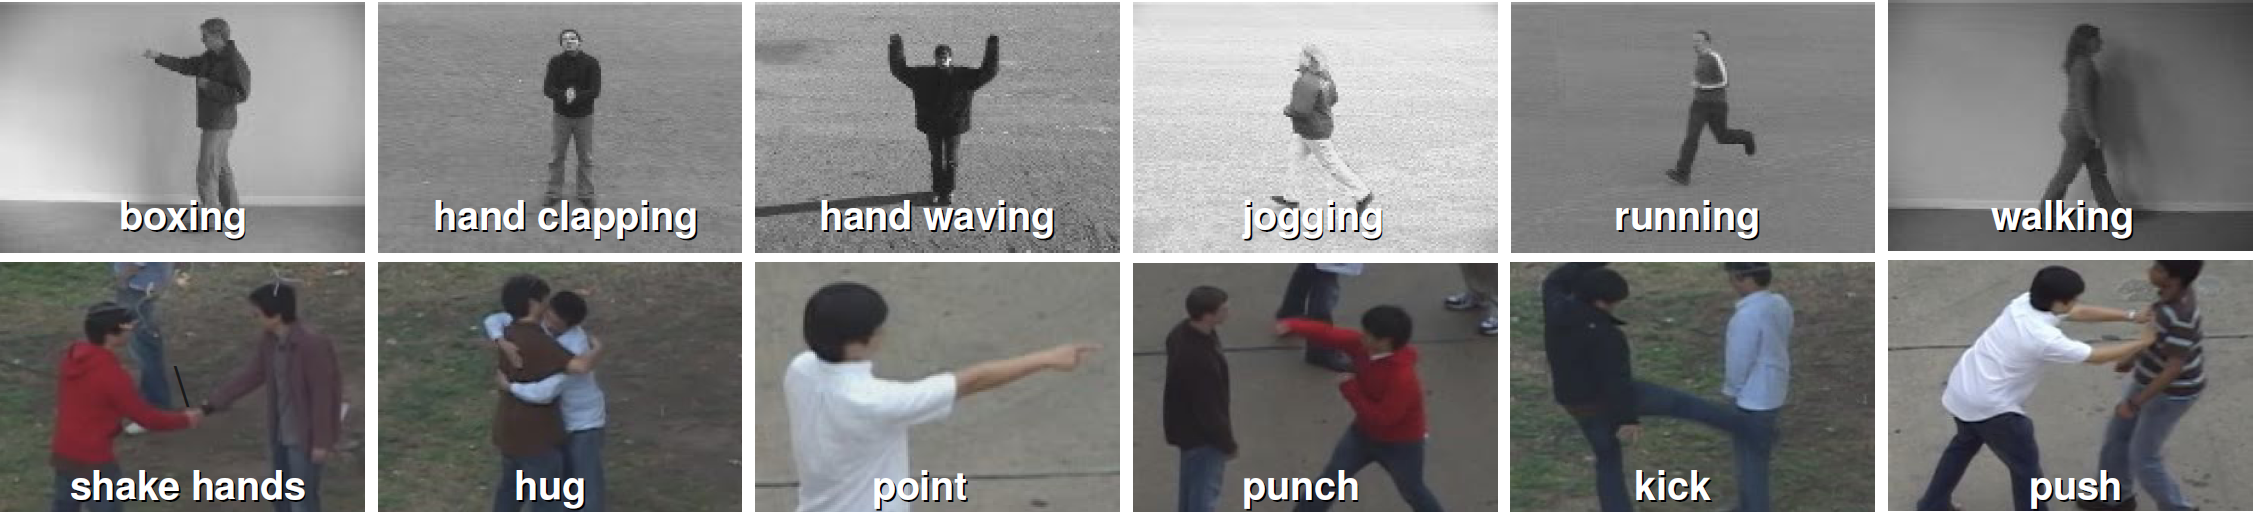
\includegraphics[width=0.8\linewidth]{fig/actreg/frames.png}
\caption{Example frames of KTH (top row) and UT-interaction (bottom row) data set}
\label{img:frames}
\end{figure}
%%%%%%%%%%%%%%%%%%%%%%%%%%%%%%%%%%%%%%%%%%%%%%%%%%%%%%%%%%%
\subsection{KTH}
% dataset introduction KTH
The KTH data set, a common benchmark for action recognition research, involves sequences of six action classes taken with camera motions, scale, appearance and subject variations (see figure~\ref{img:frames} (top)). 
%All sequences were taken at 25fps frame rate having a length of 19 seconds on average.
To demonstrate the method for continuous action recognition by a short response time, subsequences with length less than 2 seconds were extracted from the original sequences on the fly. The subsequences from training videos were used to train the classifiers. Similar subsequences were extracted from testing videos for classification. Histograms $\mathrm{B}$ and $\mathrm{H}_m(\mathrm{U})$ were computed efficiently using dynamic programming. We used leave-one-out cross validation. Most published results in the literature were reported at the sequence level, class label was assigned to the whole testing video instead of individual short subsequences. To put the proposed method in context, two different accuracies are measured: (1) ``snippet'' accuracy that is directly measured at small subsequences level; and (2) sequence level accuracy, which assigns a class label to the testing video by majority voting from subsequences' classification labels.
%%%%%%%%%%%%%%%%%%%%%%%%%%%%%%%%%%%%%%%%%%%%%%%%%%%%%%%%%%%
% Confusion matrices
%%%%%%%%%%%%%%%%%%%%%%%%%%%%%%%%%%%%%%%%%%%%%%%%%%%%%%%%%%%
\begin{figure}
\centering
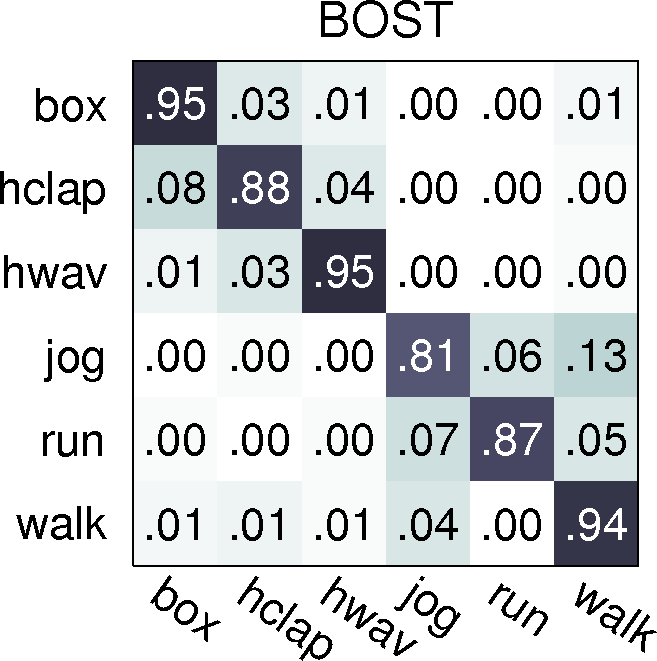
\includegraphics[width=0.2\linewidth]{fig/actreg/bost.png}
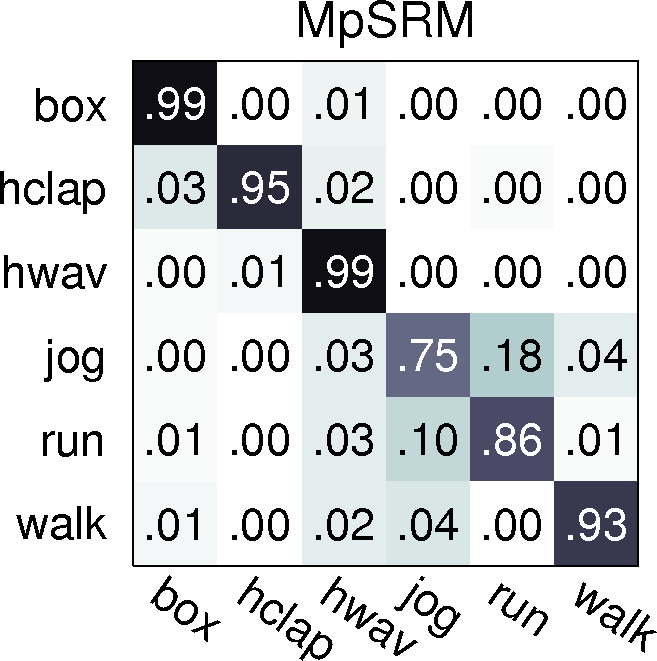
\includegraphics[width=0.2\linewidth]{fig/actreg/mpsrm.png}
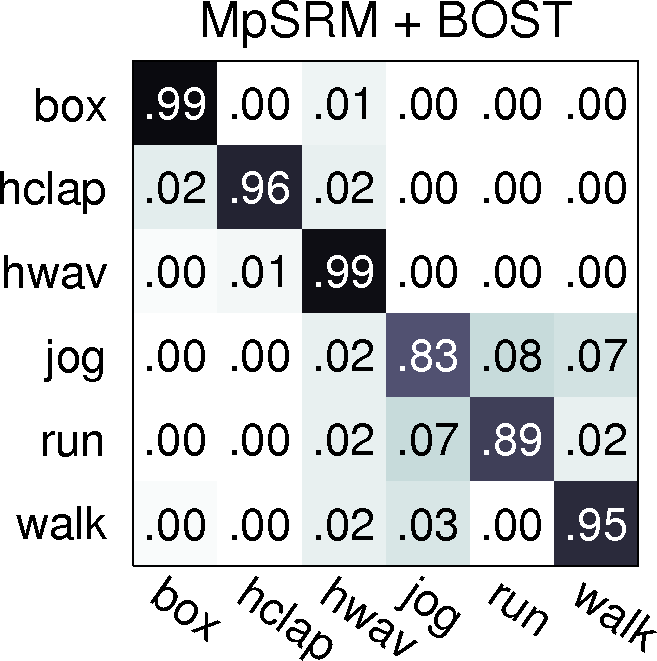
\includegraphics[width=0.2\linewidth]{fig/actreg/combine.png}
\caption{Confusion matrices of BOST (left), MpSRM (middle), and combined classification(right) on KTH dataset}
\vspace{-3mm}
\label{img:confusion}
\end{figure}
%%%%%%%%%%%%%%%%%%%%%%%%%%%%%%%%%%%%%%%%%%%%%%%%%%%%%%%%%%%
%%%%%%%%%%%%%%%%%%%%%%%%%%%%%%%%%%%%%%%%%%%%%%%%%%%%%%%%%%%
% accuracy table: KTH
%%%%%%%%%%%%%%%%%%%%%%%%%%%%%%%%%%%%%%%%%%%%%%%%%%%%%%%%%%%
\begin{table}
\centering
{\footnotesize
\begin{tabular}{|c|c|c|c|c|c|c|c|c|}
\hline
Method & box & hclp & hwav & jog & run & walk & \textbf{ Overall} & Protocol \\
\hline
\textbf{ \color{blue} MpSRM + BOST} & \textbf{ \color{blue} 100.0} & \textbf{ \color{blue}96.0} & \textbf{ \color{blue}100} & \textbf{ \color{blue}86.0} & \textbf{ \color{blue}95.0} & \textbf{ \color{blue}97.0} & \textbf{ \color{blue}95.67} & sequence\\
\textbf{ \color{blue} MpSRM + BOST} & \textbf{ \color{blue} 99.0} & \textbf{ \color{blue} 96.6} & \textbf{ \color{blue}98.9} & \textbf{ \color{blue}82.6} & \textbf{ \color{blue}89.5} & \textbf{ \color{blue}94.8} & \textbf{ \color{blue} 93.55} & snippet\\
MpSRM & 99.0 & 96.1 & 98.7 & 74.6 & 85.9 & 92.2 & \textbf{ 91.10} & snippet\\
SRM{Ryoo2009} & 96.0 & 95.0 & 97.0 & 78.0 & 85.0 & 92.0 & \textbf{ 90.5} & sequence\\
\hline
Mined features (2009) \cite{Gilbert2009} & 100.0 & 94.0 & 99.0 & 91.0 & 89.0 & 94.0 & \textbf{ 96.70} & sequence\\
CCA (2007) \cite{Kim2007} & 98.0 & 100.0 & 97.0 & 90.0 & 88.0 & 99.0 & \textbf{ 95.33} & sequence\\
Neighbourhood** (2010) \cite{Kovashka2010} & - & - & - & - & - & - & \textbf{ 94.53} & sequence\\
Info. maximisation (2008) \cite{Liu2008} & 98.0 & 94.9 & 96.0 & 89.0 & 87.0 & 100.0 & \textbf{ 94.15} & sequence\\
Shape-motion tree (2009) \cite{Lin2009} & 96.0 & 99.0 & 96.0 & 91.0 & 85.0 & 93.0 & \textbf{ 93.43} & sequence\\
Vocabulary forest (2008) \cite{Mikolajczyk2008} & 97.0 & 96.0 & 98.0 & 88.0 & 93.0 & 87.0 & \textbf{ 93.17} & sequence\\
Point Clouds (2009) \cite{Bregonzio2009} & 95.0 & 93.0 & 99.0 & 85.0 & 89.0 & 98.0 & \textbf{ 93.17} & sequence\\
pLSA-ISA (2007) \cite{Wong2007} & 96.0 & 92.0 & 83.0 & 79.0 & 54.0 & 100.0 & \textbf{ 83.92} & sequence\\
\hline
\multicolumn{9}{p{0.9\linewidth}}{\scriptsize * The length of subsequences called snippet is about 50 frames. To balance accuracy, speed and generality, the depth of random forest classifier = $8$; For k-means forest classifier: K = $10$, depth = $3$. ** Classifiers were trained by a split dataset in separate scenarios.
}\\
\end{tabular}
}
\caption{Accuracies on KTH data set by the proposed method and state-of-the-art methods. Leave one out cross validation (LOOCV) scheme was used.}
\label{tab:compare}
\end{table}
%%%%%%%%%%%%%%%%%%%%%%%%%%%%%%%%%%%%%%%%%%%%%%%%%%%%%%%%%%%

Table \ref{tab:compare} presents a detailed comparison of accuracies between our method and other state-of-the art approaches. The MpSRM+BOST model gives a very competitive accuracy, even only short subsequences are used for recognition. The confusion matrices in figure \ref{img:confusion} shows how MpSRM and BOST complement each other to attain an optimised accuracy. Quantisation effects are soothed by the multi-tree characteristics and pyramid matching of the proposed method, compared to the original Spatiotemporal Relationship Match method{Ryoo2009}.

Table \ref{tab:speed} summarises the experiment results on recognition speed. Different from other sequence-level recognition approaches, a more realistic metric is designed to measure the algorithm efficiency. All recognition stages (including feature detection, feature extraction and classification) are timed, and the average speed is defined as $(\mbox{\textit{ total number of subsequences}})/$ $(\mbox{\textit{ total recognition time}})$ \textbf{FPS}. It shows that the proposed method runs at 10 to 20 frames per second. The introduction of STF has greatly improved the speed for feature extraction and codeword generation, outperforming the k-means visual codebooks (see also Table~\ref{tab:codebook}). Using random forest and kernel k-means forest has provided faster solutions to match and classify multi-dimensional histograms over the traditional nearest neighbour and SVM. 
%%%%%%%%%%%%%%%%%%%%%%%%%%%%%%%%%%%%%%%%%%%%%%%%%%%%%%%%%%%
% Speed table
%%%%%%%%%%%%%%%%%%%%%%%%%%%%%%%%%%%%%%%%%%%%%%%%%%%%%%%%%%%
\begin{table}
\centering
{\footnotesize
\begin{tabular}{|c|c|c|c|c|c|c|}
\hline
Dataset & V-FAST  & STF and BOST & MpSRM & Random & k-means & \textbf{ Total }\\
 & feature detection &   &  & forest & forest & \textbf{ FPS}\\
\hline
KTH & 66.1 & 59.3 & 194.17 & 1137.6 & 67.1 & \textbf{ 18.98 } \\
UT-interaction & 35.1 & 25.8 & 35.1 & 612.2 & 428.1 & \textbf{ 10.02 } \\
\hline
\end{tabular}
}
\caption{A list of the average recognition speed at different stages in frame per second (FPS)}
\label{tab:speed}
\end{table}
%%%%%%%%%%%%%%%%%%%%%%%%%%%%%%%%%%%%%%%%%%%%%%%%%%%%%%%%%%%
%%%%%%%%%%%%%%%%%%%%%%%%%%%%%%%%%%%%%%%%%%%%%%%%%%%%%%%%%%%
% accuracy table: UT-interaction
%%%%%%%%%%%%%%%%%%%%%%%%%%%%%%%%%%%%%%%%%%%%%%%%%%%%%%%%%%%
\begin{table}
\centering
{\footnotesize
\begin{tabular}{|c|c|c|c|c|c|c|c|c|}
\hline
Method & shake & hug & point & punch & kick & push & \textbf{ Overall} & Protocol \\
\hline
\textbf{ \color{blue} MpSRM+BOST} & \textbf{ \color{blue} 100.0} & \textbf{ \color{blue}65.0} & \textbf{ \color{blue}100.0} & \textbf{ \color{blue}85.0} & \textbf{ \color{blue}75.0} & \textbf{ \color{blue}75.0} & \textbf{ \color{blue}83.33} & sequence\\
MpSRM & 90.0 & 50.0 & 85.0 & 65.0 & 70.0 & 40.0 & \textbf{ 66.67} & sequence\\
BOST & 80.0 & 50.0 & 100.0 & 65.0 & 25.0 & 35.0 & \textbf{ 59.16} & sequence\\
\hline
*SRM{Ryoo2009} & 75.0 & 87.5 & 62.5 & 50.0 & 75.0 & 75.0 & \textbf{ 70.8} & sequence\\
\hline
\multicolumn{9}{p{0.9\linewidth}}{\scriptsize * An unsegmented UT-interaction dataset was used in the experiments}\\
\end{tabular}
}
\caption{Accuracies on UT-interaction dataset. Leave one out cross validation (LOOCV) scheme were used.}
\label{tab:utcompare}
\end{table}
%%%%%%%%%%%%%%%%%%%%%%%%%%%%%%%%%%%%%%%%%%%%%%%%%%%%%%%%%%%
\subsection{UT-interaction Data set}
% dataset introduction UT
The UT-interaction data set contains six classes of realistic human-human interactions, including shaking hands, pointing, hugging, pushing, kicking and punching (see figure~\ref{img:frames} (bottom)). Some challenging factors of this data set include moving background, cluttered scene, camera jitters/zoom and different clothing. In the experiments, the segmented UT-interaction data set was used for evaluating the recognition accuracy and speed of our method. As reported in table \ref{tab:utcompare}, the proposed method marked the best accuracy in recognising challenging realistic human-human interactions. Under complex human interactions, MpSRM using both local-appearance and structural cues appeared to be more stable than BOST that uses only local-appearance. However, there still exist improvements in overall recognition accuracies in the combined approach. The method runs at high speed more than 10 frames per second from table \ref{tab:speed}. The recognition speed on this data set over KTH has dropped due to extra interest points from other moving objects in the scene.

\section{Conclusion}
\label{sec:discussion}
%advantages: fast, fully utilises structural information
%limitation: still have some lookahead, not so powerful features, localisation not optimised
This paper has presented a novel solution for action recognition. Different from other published approaches, a major strength of our method is the run-time speed. Real-time performance is achieved by semantic texton forest which works on video pixels generating visual codewords in an extremely fast manner. MpSRM is proposed to capture both spatiotemporal structures and local-appearances of actions and ease quantisation effects based on STF. Furthermore, a novel fast interest point detector and application of random forest and kernel k-means forest classifiers contribute to the acceleration of recognition speed. Experimental results show the comparable accuracies of the proposed method compared to state-of-the-arts. A future challenge will be tackling more complex realistic human actions and partial occlusions, as well as requiring continuous action localisation with a real-time performance.


\chapter{3-D Pose Estimation}
\section{Introduction}

\begin{figure*}[ht]
	\vspace{-2mm}
	\centering
	\begin{minipage}[b]{0.42\linewidth}
	\centering
	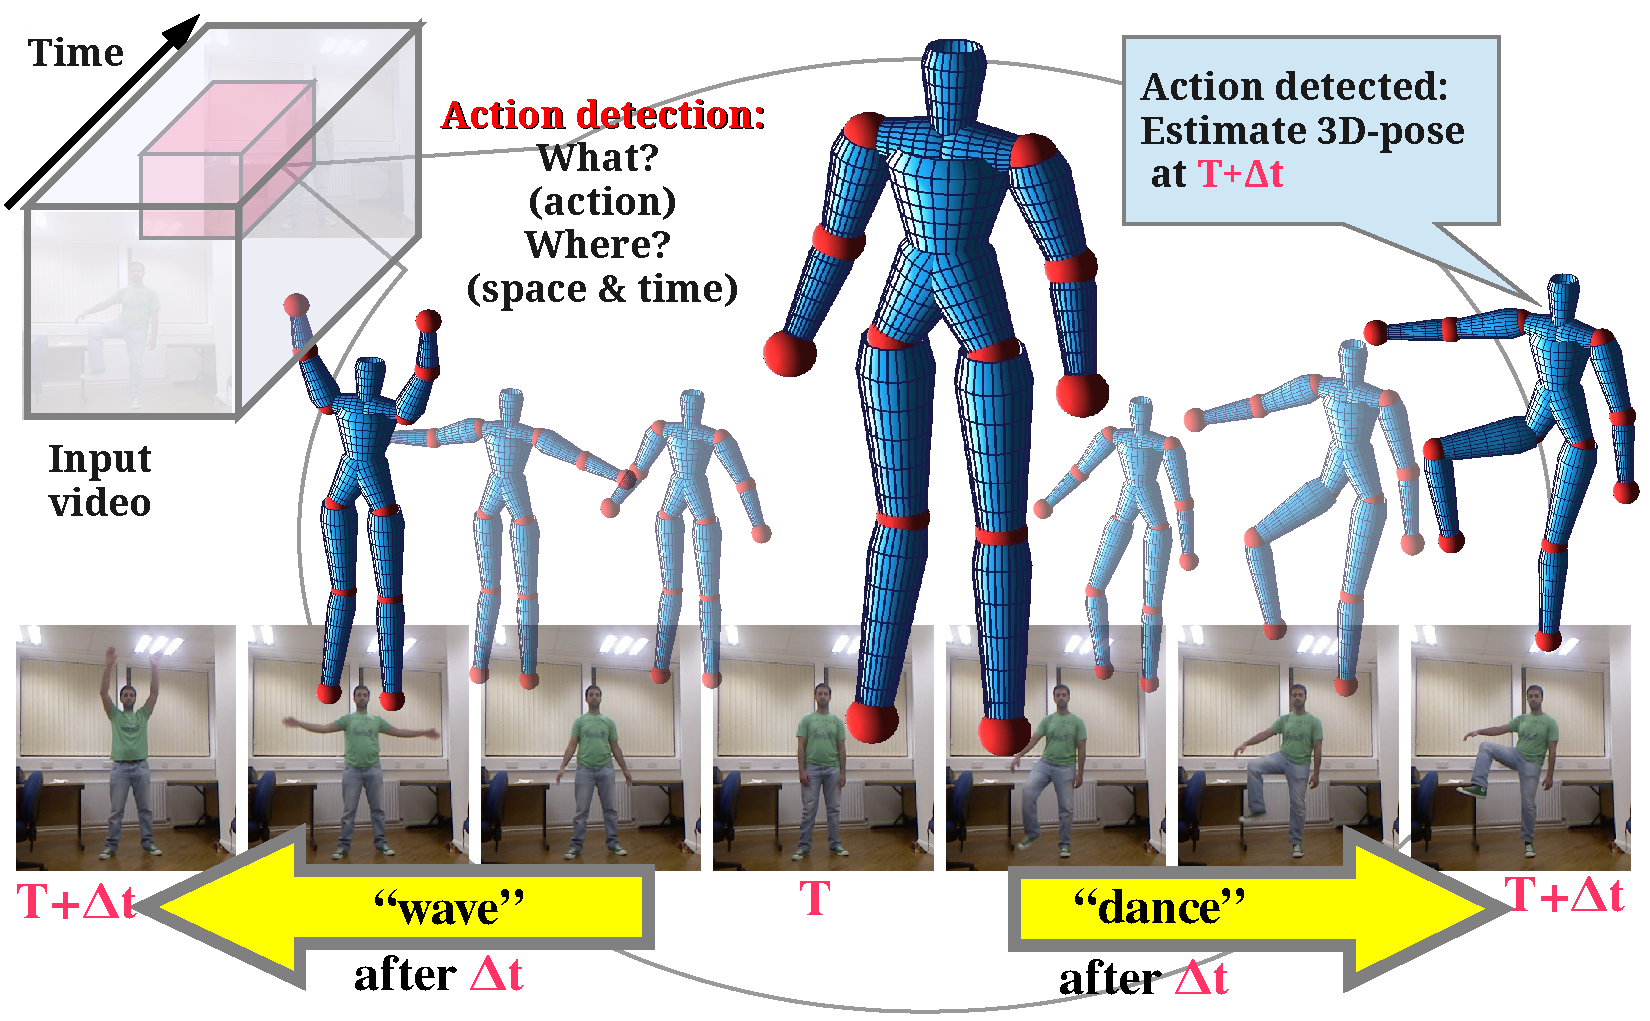
\includegraphics[width=1\linewidth]{fig/poseest/figure1_actionexplain.pdf}
	\captionof{figure}{Action detection helps 3D pose estimation by providing the spatiotemporal structure of actions.} 
	\label{fig:figure1_actionexplain}
	\end{minipage}
	\begin{minipage}[b]{0.57\linewidth}
	\centering
	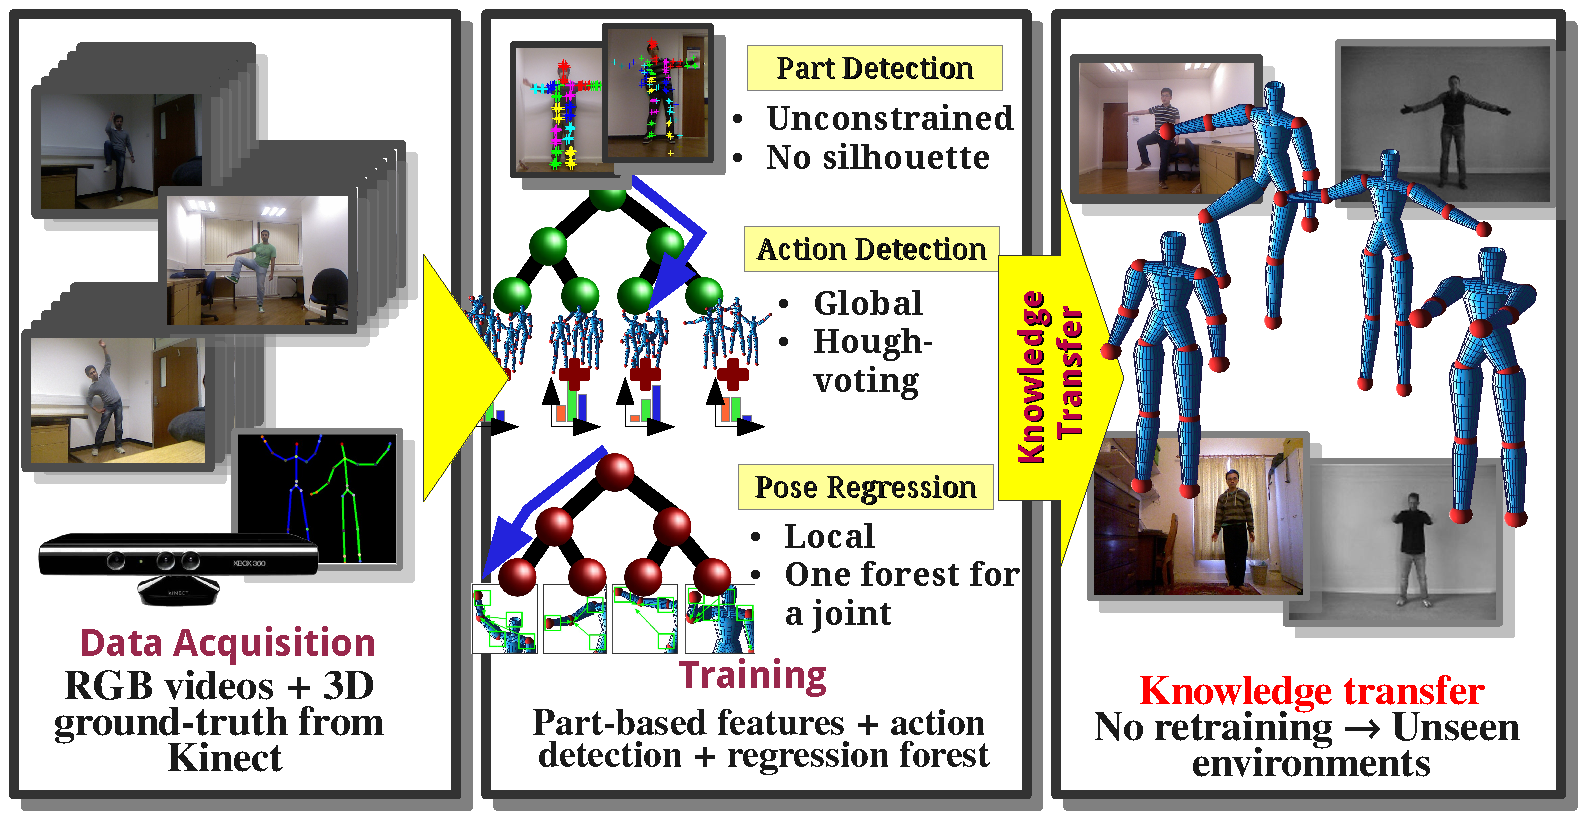
\includegraphics[width=1\linewidth]{fig/poseest/figure2_transferexplain.pdf}
	\captionof{figure}{Knowledge transfer capability of the proposed method} 
	\label{fig:figure2_transferexplain}
	\end{minipage}
\end{figure*}

%------------- backup 
%\begin{figure}[ht]
%	\centering
%	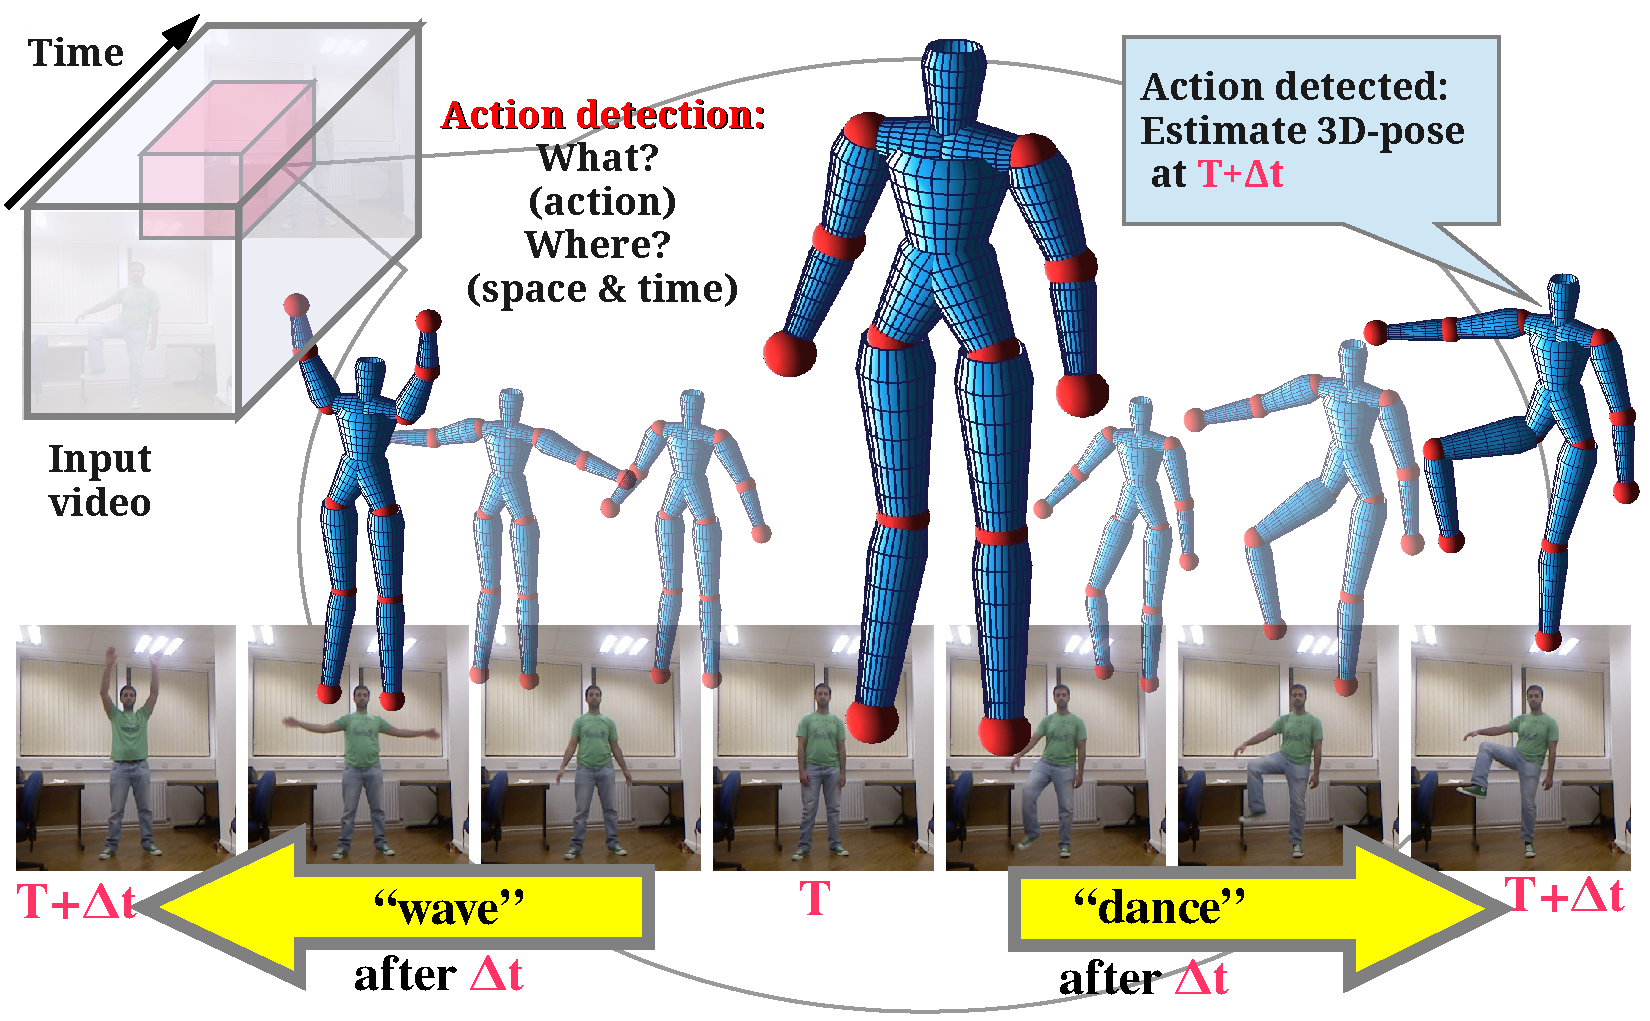
\includegraphics[width=1\linewidth]{fig/poseest/figure1_actionexplain.pdf}
%	\caption{Action detection helps 3D pose estimation by providing the spatiotemporal structure of actions.} 
%	\label{fig:figure1_actionexplain}
%\end{figure}
%-------------backup end

%\subsection{Motivations}
3D human pose estimation (HPE) has been a longstanding challenge in computer vision.
3D HPE aims to infer a human pose, represented by joint positions or angles, from input images or videos.  
%Articulated body pose estimation has been a longstanding problem in computer vision with various applications such as video analysis, motion capture and surveillance.
% what is 3D HPE? Do we need to explain that?  
Contemporary methods commonly approach 3D pose estimation as a regression or a manifold learning scenario, features are embedded to a parametrised 3D pose space. 
%, poses are estimated by learning a mapping is learnt from the appearance space to the 3D pose space. 
However, learning mappings between high-dimensional spaces is an essentially ill-posed problem \cite{Elgammal2004}. Additional priors are needed to optimise a correct pose from multiple hypotheses. 
These priors are crucial to pose estimation, however, they also require a much controlled environment to capture compatible data: clean background segmentation, a calibrated multi-camera network, and depth sensor. 
Furthermore, if there are changes to the imaging environment, the whole pose estimator has to be retrained, making the pose estimation algorithm not scalable. 
%Furthermore, the pose estimator has to be retrained if the imaging environment changes, making the pose estimation algorithm not scalable.  

%including multi-view videos, body segmentation and specialized hardware. 
%Ideal imaging conditions, such as a clean background and calibrated camera system, seldom exist in realistic applications. 

%\begin{figure}[th]
%	\centering
%	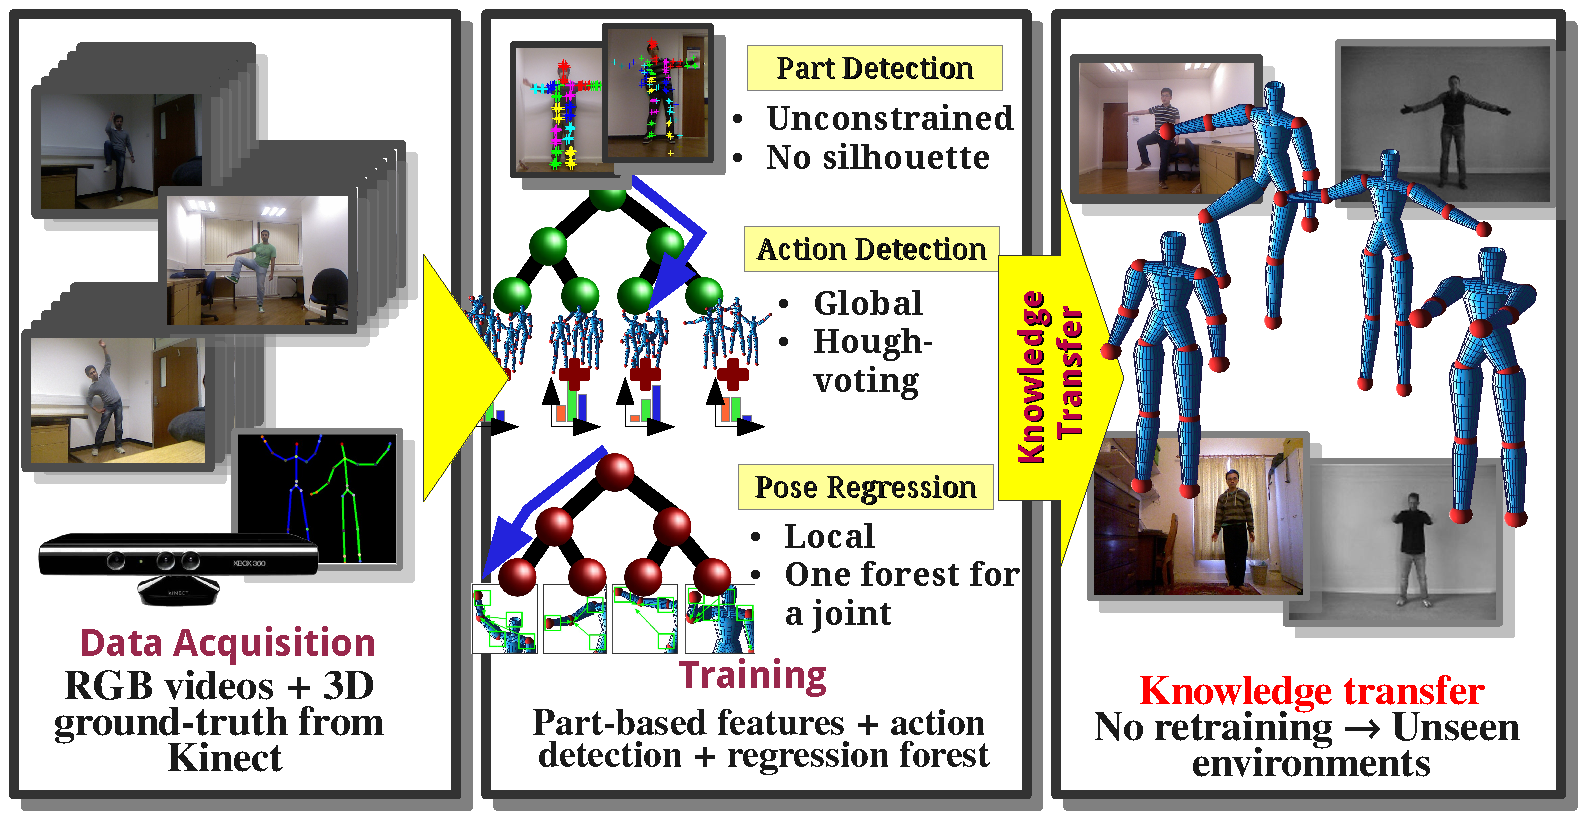
\includegraphics[width=1\linewidth]{fig/poseest/figure2_transferexplain.pdf}
%	\caption{Knowledge transfer capability of the proposed method} 
%	\label{fig:figure2_transferexplain}
%\end{figure}
In this paper, we present a new method that incorporates action detection and 2D part-based pose estimation techniques for realistic, video-based 3D pose estimation. Our contributions are three-folds: 
\paragraph{Action detection.} Firstly, we combine action detection with 3D pose estimation to utilise the strong spatiotemporal structures of actions.
The analysis of human pose and action are two closely interrelated areas in computer vision. Although there exist initial studies in using human poses for recognising actions \eg \cite{Yao2012, Wang2012}, the opposite direction, \ie using actions to help pose analysis, 
is still an aspect that many methods have overlooked. 
An atomic action is considered as a time series of poses, with particular starting/ending poses and their transitions in-between. By detecting an atomic action in video,  a strong 3D pose prior per each frame is obtained. 
%in pose estimation. 
%In computer vision, learning pose and action are two closely interrelated areas.
%, 3D poses can be estimated by transferring the knowledge learned from action. 
%However, the temporal structures of human poses is an aspect that many methods have overlooked. 
In addition to kinematic constraints, action determines the temporal structure of a series of poses. For instance, in figure \ref{fig:figure1_actionexplain}, action detection simultaneously estimates the action category and the space-time location of an action, supporting pose estimation within the action's time span.
%estimates both the category and temporal location of an action. are detected from input video snippets, giving a strong prior for pose estimation. Besides recognising action categories, an action detector also estimates the temporal location of an action, providing a respecitve pose hypothsis per frame.  
%We therefore propose action detection in video as a strong resonable prior for 3D pose estimation.
\paragraph{2D part detection.} Secondly, we apply 2D part-based pose estimation techniques to infer 3D articulated poses. 
Holistic shape features, such as silhouettes which rely on background segmentation, are replaced by a deformable part model (DPM), \eg \cite{Yang2011}, to maximise flexibility. Our method is therefore knowledge transferable, learned models can be reused in unseen environments without retraining (see figure~\ref{fig:figure2_transferexplain}). 
\paragraph{Cross-modality regression forest.} 
Finally, we refine 3D human poses from 2D part detections using cross-modality regression forests.
To the best of our knowledge, this is the first application of regression forest~\cite{Criminisi2011} across modalities to 3D HPE problem.  
Estimating 3D human pose is essentially a cross-modality regression problem: 
\emph{3D structure} of a human pose is inferred using features extracted from its \emph{2D appearance} 
%Learning a regression across the two modalities is difficult, because the relationship between them are implicit.
Since the relationship between the two spaces are implicit, learning a robust regression model across two modalities becomes a challenging issue. 
The regression forests estimate joint positions in 3D from detected 2D parts, which are combined with action detection to optimise 3D pose estimation. 
The outputs of both forests, and their combined results, are formulated in a probabilistic framework. 
While some methods yield a point estimate in the pose space, our approach outputs joint positions as probability distributions in 3D space. 
%We design a algorithm to refine 3D joint positions using cross-modality regression forest. 
% 3D joint positions are refined, from detected 2D parts and action categories, using a cross-modality regression forest. 

%The rest of the paper is organised as follows: 
%relevant work is reviewed in section \ref{sec:review}. 
%The proposed method is detailed in section \ref{sec:method}. Section \ref{sec:eval} describes the experimental framework and performance evaluation. Finally, section \ref{sec:conclusions} concludes with discussions and furture work. 

\section{Literature Review}\label{sec:review}
\paragraph{Early methods.} 
Part-based 2D pose analysis has been studied for decades, examples of early approaches include \eg pictorial structure \cite{Fischler1973} and template matching \cite{Ioffe1999}. 
However, these methods are limited due to the lack of an automatic part detector, which implies manual labelling required for both training and testing data. 
%However, these methods are greatly limited as they require manuall labeled data.
3D human pose estimation is more complicated than its 2D counterpart due to occlusions and high dimensionality. 
To estimate 3D pose from video data, various techniques have been proposed, \eg image edges \cite{Hogg1983} and silhouettes \cite{Navaratnam2006}. Approaches for traditional 3D human pose estimation are discussed in \cite{Poppe2007}. 
Cross-modality approach had not been explored until \cite{Micilotta2006}, where 2D face and hand detectors were used to infer a simple 3D pose of upper body.  

%The spatial arrangements of body parts have been widely used in 2D human pose anaylsis. For example, Fischler and Elschlager \cite{Fischler1973} conceptualized \emph{pictorial structure} for modeling the spatial structure of human pose, Ioffe et al. \cite{IOffe1999} described body parts as a collection of image templates. 
%However, the effectiveness of these approaches were greatly limited due to the lack of robust detectors for different body parts, manual labelling of body parts was often required. 
%On the other hand, 3D pose estimation is more complicated than its 2D counterpart, due to occlusions and a high dimensionality in the pose space. Various methods have been developed: Hogg \cite{Hogg1983} used image edges to compute the 3D pose of a walking person from a carefully controlled environment. 
%Micilotta et al. \cite{Micilotta2006} used several part detectors, e.g. face and hand detectors, to infer a simple 3D pose of the person upper body. A regression algorithm was presented by Navaratnam et al. \cite{Navaratnam2006} to compute 3D poses from silhouettes. 
%\subsubsection{Recent approaches}

More recent techniques of human pose estimation are discussed below according to the techniques or representations used.

\paragraph{Silhouette or depth image.} 
Holistic shapes, silhouettes in particular, are common features for 3D pose estimation. 
Current approaches achieve state-of-the-art performance by combining silhouettes with new features or constraints, including motion templates \cite{Rogez2012}, pedestrian detectors \cite{Andriluka2010}, shape-contents \cite{Agarwal2006} and user interaction \cite{Guan2009}.  
%State-of-the-art performances are achieved by combining silhouettes with new features or constraints, including motion templates \cite{Rogez2012}, pedestrian detector \cite{Andriluka2010}, shape-context \cite{Agarwal2006} and user interaction \cite{Guan2009}.  
Thanks to the introduction of the Kinect sensor, using depth images emerges as a new direction for 3D HPE, as it provides inherent depth information and object segmentation. 
%Recently, several depth-based 3D HPE approaches have been introduced, such as \cite{Baak2011}, \cite{Ye2011} and \cite{Sun2012}. 
Several methods recognise 3D human poses from depth images, using techniques such as point cloud matching \cite{Baak2011, Ye2011} and random forest \cite{Taylor2012, Sun2012}. 
However, many of the above methods require an accurate image segmentation to extract shape features, thus special hardware (\eg Kinect sensor) or controlled environments are often necessary to acquire compatible training or testing data.  
%for the task.
%For instance, Bissacco et al. \cite{Bissacco2007} proposed a boosting classifier to compute human poses from both silhouettes and motion features.  
%Guan et al. \cite{Guan2009} estimated human poses and shapes simultaneously from silhouettes, assisted by manual initializations.
%A lantent structured model is described in \cite{Ionescu2011} to estimate 3D poses from silhouettes. 
%Pons et al. \cite{Pons-Moll2011} presented a pose optimization algorithm from silhouettes captured from multiple cameras. 
%Motion templates are also used in 3D pose estimation, \cite{Rogez2012} used a global motion template to recognize poses using a tree-shape ensemble of rejectors. 
%Recently, depth sensor has become a popular imaging technique for computer vision as it provides inherent depth information as well as object segmentation.  
%Several methods are proposed to estimate 3D human poses from depth images, using techniques such as point cloud matching \cite{Baak2011, Ye2011} and random forest \cite{Sun2012}. 
%However, many of these methods on both silhouette and depth require an accurate segmentation to extract shape features from input data, thus specialized hardware and unconstrained environments are often required. 

\paragraph{Multiple-cameras.} 
A common approach to resolve the pose ambiguity is to maximise the field of view by capturing multiple images simultaneously using calibrated cameras, \eg \cite{Pons-Moll2011, Sigal2012, Yao2012}. Although they achieve excellent accuracy, potential applications are restricted to a fixed, calibrated multi-camera system. 
%Resolving the pose ambiguity from multiple views is, still, a sophisicated optimization problem. Existing solutions are often computationally expensive, which further limits its applicability.   
%
%{\bf Multiple-cameras.}
%A common approach to resolve the pose ambiguity, caused by the limitation of 2D image-baed features, is to capture several images simultaneously using multiple calibrated cameras, such as 
%\cite{Pons-Moll2011, Sigal2012, Yao2012}. Accoridingly, it restricts potential applications to a fixed, calibrated multi-camera system. Furthermore, resolving the pose ambiguity from multiple views is, still, a sophisicated optimization problem. Existing solutions are often computationally expensive, which further limits its applicability.   
% Pose ambiguity is a common issue for 3D pose estimation.
%%Due to the limitation of 2D, image-based features, multiple solutions of 3D poses can be found in one estimation.
\paragraph{Action for pose estimation.}
As mentioned previously, the integration of action and pose, in particular action for pose, is still a largely unexplored area. We seek to investigate the feasibility of using \emph{action detection} to facilitate 3D human pose estimation in uncontrolled and monocular videos.
Early approaches that combines action and pose constrains include \cite{Yu2010} and \cite{Raja2011}.
The closest work to this idea is \cite{Yao2012} that uses action recognition to assist a multi-view 3D HPE algorithm. Separate regression models are trained; After an action is recognised, poses are inferred using the model of the action class estimated. 
Whilst action recognition is applied, the inputs are still images captured from a controlled, multi-camera environment. 
Instead, we perform action detection in video, by which we exploit the spatiotemporal structure of actions in addition to action class labels, to infer 3D poses.
%When the action of a person is detected in a video, it gives much information about spatiotemporal structure of that person, which is extrmely useful in the pose estimation task.  
%For instance, when a ``walking'' action is detected, it gives a strong \emph{spatial} prior to the pose estimator as outputs are limited to the ``walking'' poses. 
% However, the combination of pose estimation and action detection techniques is still a largely unexplored area. 
% \emph{temporal} used is obtained to support the pose estimator. 
%By tracing the current pose from the starting time of the action detected,
%Action recognition is performed by single images, action category labels are only used as a switch to different manifolds, where the 3D poses are estimated. 
%in uncontrolled single video. 
%a main object of our model is to estimate s by leveraging 
%has not utilized the inherit spatiotemporal structure of an \emph{action}--

\begin{figure*}[ht]
	\hspace{-2mm}
	\vspace{-3mm}
	\begin{minipage}[b]{0.27\linewidth}
		\centering
		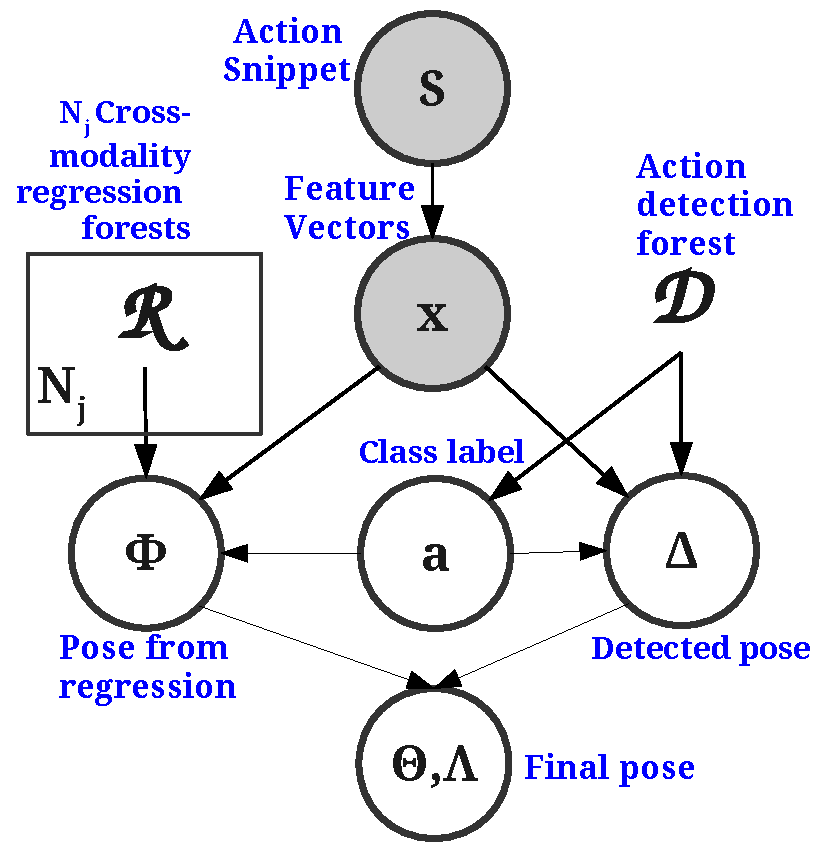
\includegraphics[width=1\linewidth]{fig/poseest/figure4.pdf}
		\captionof{figure}{Graphical representation of the proposed model} 
		\label{fig:figure4gm}
	\end{minipage}
	\begin{minipage}[b]{0.75\linewidth}
		\centering
		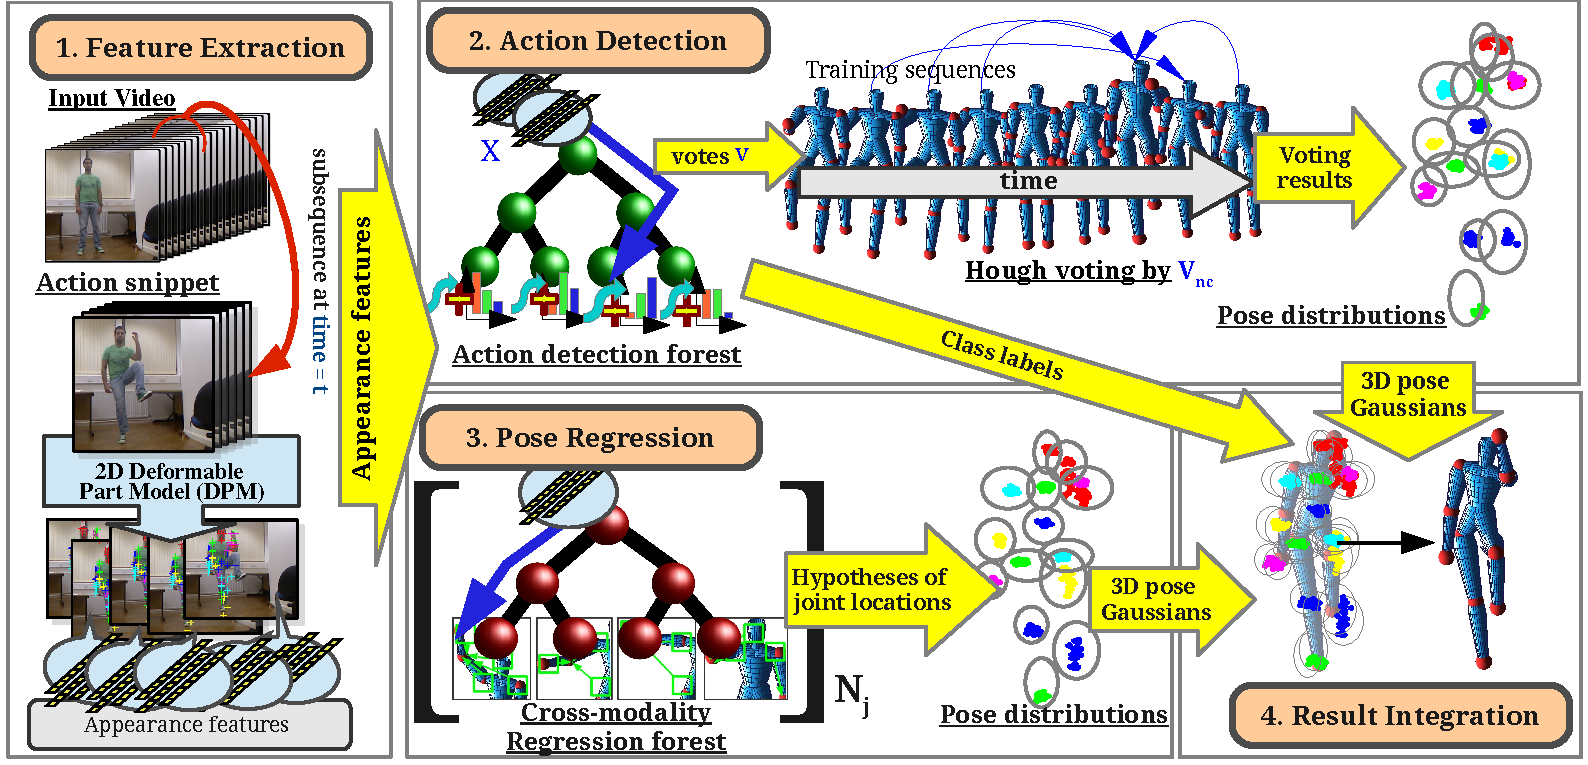
\includegraphics[width=1\linewidth]{fig/poseest/figure3_overview.pdf}
		\captionof{figure}{Overview of the proposed framework}
		\label{fig:overview}
	\end{minipage}
\end{figure*}


\paragraph{Part-based pose estimation.} 
Various methods have been introduced built upon the original seminal model of pictorial structures \cite{Felzenszwalb2000, Felzenszwalb2010}. Recent extensions include new motion features \cite{Andriluka2009}, improved part-based model learning and inference \cite{Yang2011, Sun2012a}, and pre-processing techniques (\eg face detector) \cite{Eichner2012}. 

%Current state-of-the-arts usually build upon the success of traditional methods with new features or improved models. For instance, Sapp et al. \cite{Sapp2011} modeled pictorial structure in a more complicated graph by decomposing the it into smaller, stretchable components. 
% Similarly, an branch-and-bound algorithm was proposed in \cite{Sun2012a} to extend traditional pictorial structure beyond star-shaped or tree graphs. 
% using new features 
%In \cite{Hua2007}, visual tracking is combined with part detection in order to estimate articulated human pose. 
%Ardriluka et al. \cite{Andriluka2009} revisited traditional pictorial structure using dense shape context and adaboost algorithm. 
%Eichner et al. \cite{Eichner2012} presented a multi-phase algorithm to detect 2D body parts from unconstrained images using various clues such as face detection and graph cut algorithm. 

%Despite achieving remarkable performances, particularly in uncontrolled environments, 
%As  has shown a better performance than its 3D counterpart, especially in uncontrolled environments, it is suggested that similar techniques can be applied %to improve 3D pose estimation results. As a result, recent advances in 2D pose estimation, e.g. deformable part-based models %\cite{Felzenszwalb2010}, inspired a resurgence of part-based approaches for 3D human pose estimation.   
Recent advances in 2D human pose estimation methods, particularly in uncontrolled environments, have inspired a resurgence of part-based approaches for 3D pose estimation. 
While some approaches use manually labelled 2D parts to estimate 3D poses, \eg \cite{Wei2009, Ramakrishna2012}, 
%the poselet algorithm \cite{Bourdev2009} estimate a rough 3D pose by learning 2D part templates. 
2D deformable part models are also investigated in 3D human pose estimation, for instance, \cite{Andriluka2010} uses a pedestrian detector with deformable body parts to estimate rough 3D poses in street scenes, 
\cite{Simo-Serra2012} optimises multiple pose hypotheses from 2D DPM using inverse kinematics to estimate 3D pose in a single image.
In this work, we further investigate the use of 2D DPM in a multi-action 3D HPE scenario. 

%Consequently, multi-action 3D pose estimation with deformable part model is a topic of great research potential. 
%Simo-Serra et al. \cite{Simoserra2012} estimate 3D poses in an image using multiple hypotheses obtained from a 2D pictorial structure model. 
%In addition, part-based models are also used to infer poses of walking pedestrians in videos\cite{Andriluka2010}. Meanwhile, the poselet algorithm \cite{Bourdev2009} uses templates of body parts to estimate a rough 3D pose from an unconstrained image. The above part-based approaches demonstrate a greater flexibility than holistic-based methods. Hence, part-based 3D pose estimation in a multi-action scenario has become a topic with great research potential. 

%By applying suitable inverse kinematics constraints, 3D poses can be estimated accurately from images with manually labeled parts \cite{Wei2009, RamakrishnaECCV2012}. 
%Simo-Serra et al. \cite{Simoserra2012} estimate 3D poses in an image using multiple hypotheses obtained from a 2D pictorial structure model. In addition, part-based models are also used to infer poses of walking pedestrians in videos\cite{Andriluka2010}. Meanwhile, the poselet algorithm \cite{Bourdev2009} uses templates of body parts to estimate a rough 3D pose from an unconstrained image. The above part-based approaches demonstrate a greater flexibility than holistic-based methods. Hence, part-based 3D pose estimation in a multi-action scenario has become a topic with great research potential. 
\section{Method}
\label{sec:method}
Figure \ref{fig:figure4gm} describes the graphical model of our 3D human pose estimation framework: action detection is performed to yield the rough 3D pose estimates, then cross-modality regression forests with the estimated action classes are applied to refine the 3D pose estimations. While full poses, \ie 3D coordinates of all $\njoints$ joints, are learnt in the action detection forest, one joint location is estimated per cross-modality regression forest. $\njoints$ regression forests are hence trained separately in the model. The conceptual data-flow of the proposed framework is illustrated in figure \ref{fig:overview}.

%used to refine
%After action detection, cross-modality regression forests are used to refine the rough 3D pose estimations given by the action detection process. 

\subsection{Part-based Feature Extraction}

In order to perform 3D pose estimation in different backgrounds and scenarios, input features are extracted using a 2D part-based model. 
Firstly, a deformable part model (DPM) \cite{Yang2011} is employed as an off-the-shelf method to extract body parts from input frames.
Unlike the traditional holistic silhouette-based methods, where background subtraction is preformed, our method based on body parts works at unseen and dynamic backgrounds. 
The DPM fires $\nhyp$ body part configurations per frame, each hypothesis contains $26$ locations of detected body parts as in \cite{Yang2011}. 
%hypotheses on configuration of $26$ body parts are obained per frame (the number of hypothese is dentoed ${\nhyp}$). 
Subsequently, the detected configurations are normalised with respect to the distance between the head and the waist part. 
Finally, a feature vector is computed per configuration by the pairwise distances among the normalised parts, hence the feature vector takes $325 (=26\times25/2)$ dimensions.

In the training process, every feature vector is associated with a ground truth 3D pose.
The Kinect sensor is used to acquire 3D poses simultaneously with the RGB video sequences. 
A 3D human pose is represented by the scale-normalised coordinates of the $\njoints$ joints detected by the Kinect sensor, an articulated model of $\njoints=15$ joints is used in this work. 
Every feature vector in the training dataset is assigned to the 3D pose detected and one of the $\nclass$ action categories, according to its corresponding frame and video. The feature vectors are denoted as $\fset = \{\feature_{\videoth\frameth\hypth}\}$, where $\feature_{\videoth\frameth\hypth}$ is the $\hypth$-th configuration detected in the $\frameth$-th frame of the $\videoth$-th training video. The corresponding class label and corresponding 3D pose
 are defined as  $\aset = \{\action_{\videoth\frameth\hypth} | \action_{\videoth\frameth\hypth} \in 1,\dots,\nclass \}$ and $\pset = \{\pose_{\videoth\frameth\hypth} | \pose_{\videoth\frameth\hypth} \in \realnum^{3\njoints}\}$ respectively.  
Furthermore, 3D poses $\pset$ of each action category are compressed separately into low-dimensional vectors $\ppset = \{\ppose_{\videoth\frameth\hypth}  |  \ppose_{\videoth\frameth\hypth} \in \realnum^{\pcadim} \}$ using PCA. 

% in the $\frameth$-th frame of the $\videoth$-th video :w






\subsection{Learning} 

\paragraph{Action Detection Forest.}
\label{sec:adflearn}
The action detection forest, $\forestd$, performs action categorisation and 3D pose clustering simultaneously. 
In each leaf node, the 3D pose vectors $\ppset$ are classified into the action class labels $\aset$ and cohering 3D pose vectors are grouped together.
For given data triplets $\fset$, $\ppset$ and $\aset$, we grow $\ntreed$ decision trees by recursively splitting the data into two child nodes, where candidate split functions are generated randomly, each compares a value in the feature vector $\feature$ with a threshold. The best split is chosen among the candidates by maximising a quality measure. The splitting process is performed until the new node reaches its maximum depth or minimum number of data points. Lastly, every leave node stores the votes that are required in Hough-voting for action detection during testing. 

%are grouped coherent to form a 3D pose cluster. 

%is essentially a Hough forest \cite{Gall2011}, where,

%use to classify parts and let parts vote for the center of atomatic actions in space and time. 
%hybrid of clssification and clustering forest learnt using

%for object detection  with classification capability. 
%A decision tree is grown by passing down a random subset of training data from the root node. 
%Candidate split functions are generated randomly, each compares a feature value with a threshold. 
%n a new node, the optimal split is chosen among the candidates by maximizing a quality measure. 
%Incoming training data are divided into two subsets, which are passed down to two new child nodes.  

%Both classification and detection are performed in a single decision tree. To this end,

 We propose a new integrated quality measure $\qualityad(\cdot)$ at the node $\curnode$ as:
%is proposed in equation \ref{eq:newquality}:
%\begin{align}
%	\label{eq:newquality}
%	\qualityad(\ppset_{\curnode}) & = \alpha \infogain(\ppset_{\curnode}) + (1-\alpha)\qualityjr(\ppset_{\curnode}) \\ 
%	\qualityjr(\ppset_{\curnode}) & = \displaystyle\sum_{c = 1}^{\nclass} \Psi(\Sigma(\ppset_{\curnode c})) - \nodeweight_{L}\Psi(\Sigma(\ppset_{Lc})) - \nodeweight_{R}\Psi(\Sigma(\ppset_{Rc}))\\
%	\alpha & = \max_{c}(|\aset_{\curnode} = c| / |\aset-{\curnode}|)- \min_{c} (|\aset_\curnode = c| / | \aset_{\curnode}|)
%\end{align}
\begin{align}
	\label{eq:newquality}
	\qualityad(\ppset_{\curnode}) & = (1 - \omega)\infogain(\ppset_{\curnode}) + \omega\qualityjr(\ppset_{\curnode}). 
\end{align}
The first term, $\infogain(\cdot)$, is the information gain measure used in standard classification forest \cite{Breiman2001} (here for action classification); the second term measures the improvement in 3D pose coherence when a split is performed    
\begin{equation}
	\qualityjr(\ppset_{\curnode}) = \displaystyle\sum_{c = 1}^{\nclass} \Psi(\Sigma(\ppset_{\curnode c})) - \Psi(\Sigma(\ppset_{lc})) 
- \Psi(\Sigma(\ppset_{rc})),
\end{equation} 
where $\Psi(\cdot) = \log(\det(\cdot)) $ and $\Sigma(\ppset_{\curnode c})$ is the covariance matrix of the PCA-compressed 3D pose vectors  $\ppset_{\curnode c}$ of the n-th node ($l,r$ denote the left and right split respectively) and the $c$-th action class. These measures are weighted by $\omega$ that describes the class purity of a node as
\begin{equation}
	\omega = \max_{c}(|\aset_{\curnode c}| / |\aset_{\curnode}|)- \min_{c} (|\aset_{\curnode c}| / | \aset_{\curnode}|),
\end{equation} 
where $\aset_{\curnode}$ denotes the action labels of training data in node $\curnode$ and $\aset_{\curnode c}$ the action labels of node $\curnode$ and class $c$. The first quality term in (\ref{eq:newquality})  optimises action classification performance while the second term optimises pose clustering performance within a node. Initially, classification is preferred over clustering, $\infogain(\cdot)$ is dominant when class labels are evenly distributed. However, $\omega$ gradually increases as the tree grows, shifting the learning focus to clustering. 

%$\aset_{\curnode c} = \{\action_{\curnode} = c| \action_{\curnode} \in \aset_{\curnode}\}$. 

%Information gain $\infogain$ \cite{Breiman2001} is applied initially to optimize classification performance. When class entropy decreases in deeper nodes, e.g. more than $90\%$ of the training instances belong to the same label, the second quality measure $\qualityad$ is used instead to optimize for detection accuracy: 
%where $\ppset_{\curnode c}$ represents the training dataset in current node $\curnode$ with class label $c$, it is split into two subsets 
%$\ppset_{Lc}$ and $\ppset_{Rc}$ to the left and right child nodes. 
%The compactness of 3D poses in a node is measured by the log-determinant of covariance $\log|\Sigma(\cdot)|$. 
%The quality measure is the increase in node data compactness after the split, weighted by the node size ratio $\nodeweight_{L} = |\ppset^{\curnode}_{Lc}| / |\ppset_{\curnode c}|$ and $\nodeweight_{R} = 1 - \nodeweight_{L}$.

% a small subset of data remains in each leaf node.
Once the learning is completed, the class posterior of a leaf node $\termnode$ is obtained by:  
\begin{equation}
	\label{eq:dforest_treeposterior}
	P(\action = c| \termnode) = |\aset_{\termnode c}|/| \aset_{\termnode}| 
\end{equation}
The distribution of 3D poses, given a action class-label $c$, is modelled by a Gaussian 
$\normdist(\mu({\ppset}_{\termnode c}), \Sigma(\ppset_{\termnode c}))$.
A vote $\vote_{\termnode c}$ cast by the leaf node is a  pair  
$ \vote_{\termnode c}= ( \videoth_{\termnode c}, \frameth_{\termnode c}), c = 1,...,\nclass$ such that
\begin{equation}
	(\videoth_{\termnode c}, \frameth_{\termnode c}) =  
	\displaystyle\argmin_{(\videoth, \frameth)} || \ppose_{\videoth\frameth\hypth} - \mu({\ppset}_{\termnode c}) ||_{2}
\end{equation}
$\videoth_{\termnode c}$ and $\frameth_{\termnode c}$ are the indices of the training sample that is the nearest neighbour of Gaussian mean $\mu(\ppset_{\termnode c})$. As a result, $\frameth$ is a temporal vote to the staring point of actions in sequence $\videoth$.

% = \sum_{i}^{|\ppset_{\termnode c}|} \ppset_{\termnode c i}/|\ppset_{\termnode c}|$.


%back-projected 3D poses of the above Gaussian means, such that:
%where the mean is approximated by its nearest neighbour in the training dataset.  


%\begin{equation}
%	\begin{array}{c}
%
%		\videoth_{c\termnode}, \frameth_{c\termnode}, \hypth_{c\termnode} =  
%		\displaystyle\argmin_{\videoth, \frameth, \hypth} || \ppose_{\videoth\frameth\hypth} - \overline{\ppset}_{\termnode} ||_{2}  \\
%
%		P(\ppose'| \termnode, \action_{\termnode} = c) = \normdist(\ppose',%\ppose_{\videoth_{c\termnode}\frameth_{c\termnode}\hypth_{c\termnode}},  \Sigma(\ppset_{c\termnode})) 
%
%	\end{array}
%\end{equation}


%\begin{figure*}[t]
%\begin{center}
%\vspace{5cm}
% %\includegraphics[width=0.8\linewidth]{egfigure.eps}
%\end{center}
%   \caption{Methods in details.}
%\label{fig:long}
%\end{figure*}

\paragraph{Cross-modality Regression Forest.}
\label{sec:jrflearn}
The cross-modality regression forests $\{\forestr^{(j)}|{j} = 1,\dots,\njoints\}$, inspired by \cite{Criminisi2011}, are learned to refine the 3D locations of joints. Each forest $\forestr^{(j)}$ contains $\ntreer$ trees that estimate the location of the $j$-th joint, trained independely from the dataset $\{ \pset^{(j)}, \fset, \aset\}$, where $\pset^{(j)}$ is the $j$-th joint's 3D coordinates in $\pset$. 
Split function candidates are generated in the same way as action detection using the feature vector $\feature$. 
%We assume that class esimates are given during testing by the detection forest, so . 
Although action class posteriors can be computed in the terminal nodes, it is not modelled in this method as the action detection forest $\forestd$ provides a better action recognition rate that helps the localisation accuracies of $\forestr^{(j)}$. Thus, $\qualityjr(\pset^{(j)}_{\curnode})$ is used instead to optimise the split functions for the localisation accuracy of the $j$-th joint. 
% ---- back up 
%\begin{equation}
	% \qualityjr(\pset^{(m)}_{\curnode c}) = \displaystyle\sum_{c = 1}^{\nclass} \left(  \log|\Sigma(\pset^{(m)}_{\curnode c})| - \nodeweight_{L}\log|\Sigma(\pset^{(y)}_{Lc})| - \nodeweight_{R}\log|\Sigma(\pset^{(m)}_{Rc})| \right)
%	\qualityjr(\pset^{(m)}_{\curnode}) = \displaystyle\sum_{c = 1}^{\nclass} \Psi(\Sigma(\pset_{\curnode c})) - %\nodeweight_{L}\Psi(\Sigma(\pset_{Lc})) - \nodeweight_{R}\Psi(\Sigma(\pset_{Rc}))
%\end{equation}
% ---- back up

% not neccessary
% where $\pset^{(m)}_{\curnode c}$, $\pset^{(m)}_{L c}$ and $\pset^{(m)}_{R c}$ are the training data in $\curnode$, its left child and right child respectively. 
% Since the action class labels are recognized in advanced via action detection, the quality function $\qualityjr$ aims to minimize the uncertainty in joint regression rather than classification error.
Tree growing is stopped when the current node is smaller than a certain size.
Upon completion of $\forestr^{(j)}$, the output of its leaf nodes $\termnode$ are described by the mean joint coordinates with respect to class label, given by $\mu(\pset^{(j)}_{\termnode c})$.  

%The mean $\overline{\pset^{(m)}_{\termnode c}}$ is not computed for class $c$ no data is present in $\termnode$.  


\subsection{Testing}

Video snippet, the basic unit required for action detection \cite{Schindler2008}, is a short sequence excerpted from the testing video, centered at time $\timenow$. A snippet $\snippetnow$ contains $\snippetlen$ frames such that $\snippetnow = \left\{ \sframe_{\timenow - \snippetlen/2}, \dots, \sframe_{\timenow + \snippetlen/2 - 1} \right\}$. The testing process starts with extracting features from $\snippetnow$, such that $\fset_{\snippetnow} = \{ \feature_{ij}\}$, where $i =\timenow-\snippetlen/2,...,\timenow+\snippetlen/2-1$ and $j=1,...,\nhyp$ with $\nhyp$ denotes the number of part configurations of the frame.
\paragraph{Action detection (classification).} 
\label{sec:adftest}
Action detection forest $\forestd$ performs action classification on $\snippetnow$. Let $\termnode_k[\feature_{ij}]$ be the leaf node reached by a feature $\feature_{ij}$ in the $k$-th tree of $\forestd$. The posterior of snippet action class at time $t$ is defined as 
\begin{equation}
	P(\action = c | \snippetnow, \forestd) = \sum_{k,i,j = 1}^{\ntreed, l, \nhyp}\frac {P(\action=c|\termnode_{k}[\feature_{ij}])} {\ntreed l \nhyp}. 
\end{equation} 
%Consequently, the pose found in $\sframe_{\timenow}$ can be estimated from $\snippetnow$ by action detection. 
\paragraph{Action detection (pose voting).}
A Hough-based voting scheme is designed for action detection. 
As mentioned in section \ref{sec:adflearn}, the vote $(p,q)$ stored in $\forestd$ are temporally associated with their corresponding action sequence and time frame in the training data set. Note each training frame is paired with a ground truth 3D pose. Hence, all frames $I$ can vote for a 3D pose at time $\timenow$, by applying temporal offsets  $\delta$ to the votes obtained from $\fset_{\snippetnow}$. We define a function $\Delta(\snippetnow,c)$ that returns a set of 3D pose estimates in $\pset$ for action label $c$ from Hough-voting during action detection: 
%The set of votes $\vset[\sframe_i] = \{ \videoth_{k c}[\sframe_{i}], \frameth_{k c}[\sframe_{i}]|k\!\in\!1,\dots,\nvset;c\!\in\!1,\dots,\nclass\}$ is obtained by passing down $\forestd$ the features extracted form a frame in snippet $\sframe_{i} \in \snippetnow$. 
\begin{equation}
	\Delta(\snippetnow, c) = \pset^{\Delta}_{\termnode_{k}[\feature_{(t+\delta)j}]c}
\end{equation}
where $ k = 1,...,\ntreed$, $\delta = -\snippetlen/2,...,\snippetlen/2-1$, $j = 1,...,\nhyp$. The set $\pset^{\Delta}_{\termnode_{k}[\feature_{(t+\delta)j}]c}$ denotes the $\delta$-voted (offset-ed) pose from the $\delta$-th frame in $\snippetnow$, \ie $(t\!+\!\delta)$-th frame in input video, by passing down the $k$-th tree in $\forestd$
%are the poses associated with the votes obtained from $\snippetnow$, such that
\begin{equation}
	\begin{split}
		& \pset^{\Delta}_{\termnode_{k}[\feature_{(t+\delta)j}]c} = \{\pose_{\videoth(\frameth-\delta)\hypth}\}\\ 
		\mbox{ s.t. } & (\videoth,\frameth) = \vote_{\termnode_{k}[\feature_{(t+\delta)j}]c} \mbox{ and } \action_{\videoth\frameth\hypth} = c 
\end{split} 
\end{equation} 

% ----------------- BACK UP 2
%\begin{equation}
%\pset^{\mathcal{D}}_{c} = \{ \pose^{\Delta}_{\termnode_{k}[\feature_{(t+\delta)j}]c}\}
%\end{equation}
%where $j = [1,\nhyp]$, $\delta = [-\snippetlen/2,\snippetlen/2]$,  $ k = [1,\ntreed]$. The set $\pose^{\Delta}_{\termnode_{k}[\feature_{(t+\delta)j}]c}$ denotes the $\delta$-voted (offseted) pose from the $\delta$-th frame in $\snippetnow$, \ie $(t\!+\!\delta)$-th frame in input video, by passing down the $k$-th tree in $\forestd$
%are the poses associated with the votes obtained from $\snippetnow$, such that
%\begin{equation}
%	\begin{split}
%		& \pose^{\Delta}_{\termnode_{k}[\feature_{(t+\delta)j}]c} = \pose_{\videoth(\frameth-\delta)\hypth}\\ 
%		\mbox{ s.t. } & \videoth,\frameth\in\vote_{\termnode_{k}[\feature_{(t+\delta)j}]c}, \aset_{\videoth} = c 
%\end{split} 
%\end{equation} 
%------------------ BACK UP 1
%\begin{equation}
%	\end{
%The set of all votes cast by $\snippet_\timenow$, in the 3D pose space is defined in equation \ref{eq:allDetectVotes}:
%\begin{equation}
%	\label{eq:allDetectVotes}
%	\begin{aligned}[lcl]
%		\vset_{\_{\timenow c}} & = & \{\vset^{-\delta}_{\termnode[\sframe_{t + \delta}]};\; \delta \in [-\timenow/2,\timenow/2 )\} \\
%		\vset^{-\delta}_{\termnode[\sframe_{t + \delta}]} & = & \{\pose_{\videoth_{c\termnode}\frameth_{c(\termnode-i)}\hypth_{c\termnode}}; \; c = i, \dots, \nclass \}
%	\end{aligned} 
%\end{equation}
Elements returned from $\Delta(\snippetnow, c)$ represent 3D pose estimations at time $\timenow$. A 3D pose $\posead_{\timenow}$ is hence modelled by $\njoints$ independent Gaussians with respect to its joints. 
\begin{equation}
	\begin{split}
		& P( \posead^{(j)}_{\timenow}| \snippetnow, \action = c,\forestd) \\ 
	 & = \normdist(\posead^{(j)}_{\timenow}; \mu(\Delta^{(j)}(\snippetnow,c)), \Sigma(\Delta^{(j)}(\snippetnow,c))
\end{split} 
\end{equation}
where $\posead_{\timenow}^{(j)}\in\realnum^{3}$ is the $j$-th joint in $\posead_{\timenow}\in\realnum^{3\njoints}$.
% backup---------------------------
%\begin{equation}
%	\begin{split}
%		& P( \posead^{(j)}_{\timenow}| \snippetnow, \action = c,\forestd) \\ 
%	 & = \normdist(\posead^{(j)}_{\timenow}; \mu(\pset^{\mathcal{D}(j)}_{c}), \Sigma(\pset^{\mathcal{D}(j)}_{\timenow c}))
%\end{split} 
%\end{equation}
%where $\posead_{\timenow}^{(j)}\in\realnum^{3}$ is the $j$-th joint in $\posead_{\timenow}\in\realnum^{3\njoints}$.
% end of back up
\paragraph{Cross-modality Regression.}
\label{sec:jrftest}
Estimation of current 3D pose by the regression forest, $\posepr_{\timenow}$, is performed on per-frame basis. 
Passing down features of current $t$th frame $\{\feature_{ti}|i = 1,...,\nhyp\}$, the set of pose estimates for class $c$ is returned by the function $\Phi(\snippetnow, c)$
\begin{equation}
	\label{eq:regressset}
	% back up! 
	%\pset^{\mathcal{R}(j)}_{c} = \{\mu({\pset^{(j)}_{\psi c}})|\psi \in \termnode[\feature \in \fset_{\snippetnow}]\}
	\Phi^{(j)}(\snippetnow, c)\!=\!\ \pset^{(j)}_{\termnode_{k}[\feature_{ti}]c},  i\!=\!1,...,\nhyp,k\!=\!1,...,\ntreer
\end{equation} 
The distribution of votes for the $j$-th joint is described by an Gaussian: 
\begin{equation}
	\begin{split}
		% & P( \posepr_{\timenow}^{(j)}| \snippetnow, \action = c, \forestr)\\ 
		% & = \normdist(\posepr_{\timenow}^{(j)};\mu(\pset^{\mathcal{R}(j)}_{c}),\Sigma(\pset^{\mathcal{R}(j)}_{c})
		& P( \posepr_{\timenow}^{(j)}| \snippetnow, \action = c, \forestr)\\ 
		& = \normdist(\posepr_{\timenow}^{(j)};\mu(\Phi^{(j)}(\snippetnow, c)),\Sigma(\Phi^{(j)}(\snippetnow,c))
\end{split}
\end{equation}




\paragraph{Combined Pose Estimation.}

Three-dimensional human poses are estimated globally via action detection, and locally by the joint regression forests. 
Assuming $\posepr_{\timenow}$ and $\posead_{\timenow}$ are independent, 
the probability of both observations coincide at $\posez$ is 
\begin{equation}
	\label{eq:combination}
	\begin{aligned}[rl] 
		& P( \posead_{\timenow}\!=\!\posepr_{\timenow}\!=\!\posez, \action\!=\!c| \snippetnow, \forestr, \forestd)\\ 
		= & P(\action\!=\!c | \snippetnow, \forestd) \prod_{j = 1}^{\njoints} P( \posez^{(j)} | \snippetnow, \action\!=\!c, \forestr) \\
			 & \hspace{20mm} P( \posez^{(j)}  | \snippetnow, \action\!=\!c, \forestd) \\
		% = &  P(\action = c | \_\timenow, \forestd) \prod_{j= 1} ^{\njoints}\normdist(\posez_{\timenow}^{(j)};\:\overline{\rset^{(j)}_{\sframe_{\timenow}}},\Sigma(\rset^{(m)}_{\sframe_{\timenow}})) \normdist(\posez^{(j)}_\timenow; \overline{\vset^{(m)}_{\snippet_\timenow}}, \Sigma(\vset^{(m)}_{\snippet_\timenow}))\\ 
		= &  P(\action\!=\!c | \snippetnow, \forestd) \prod_{j = 1}^{\njoints} \normdist(\posez^{(j)}; \finalpose^{(j)}_{\timenow c}, \finalvariance^{(j)}_{\timenow c})
	\end{aligned}
\end{equation} 
% ---- back up --- 
%\begin{equation}
%	\label{eq:combination}
%	\begin{aligned}[rl] 
%		& P( \posead_{\timenow}^{(m)} = \posez^{(m)}_{\timenow}, \posepr^{(m)}_{\timenow} = \posez^{(m)}_{\timenow}, \action_{\timenow} = c| \_\timenow, \forestr, \forestd)\\ 
%		= & P( \posead_{\timenow}^{(m)} | \posepr^{(m)}_{\timenow}\_\timenow, \action_{\timenow} = c, \forestd, \forestr) P( \posepr^{(m)}_\timenow | \snippet_\timenow, \action_{\timenow} = c, \forestd) P(\action_{\timenow} = c | \snippet_\timenow, \forestd) \\
%		= & P( \posez_{\timenow}^{(m)} | \_\timenow, \action_{\timenow} = c, \forestr) P( \posez^{(m)}_\timenow | \snippet_\timenow, \action_{\timenow} = c, \forestd) P(\action_{\timenow} = c | \snippet_\timenow, \forestd)\\ 
%		= & \normdist(\posez_{\timenow}^{(m)};\:\overline{\rset^{(m)}_{\sframe_{\timenow}}},\Sigma(\rset^{(m)}_{\sframe_{\timenow}})) \normdist(\posez^{(m)}_\timenow; \overline{\vset^{(m)}_{\_\timenow}}, \Sigma(\vset^{(m)}_{\snippet_\timenow})) P(\action_{\timenow} = c | \snippet_\timenow, \forestd)\\ 
%		= & \normdist(\posez^{(m)}_{\timenow}; \mu^{(m)}_{\timenow}, \sigma^{m}_{\timenow}) P(\action_{\timenow} = c | \_\timenow, \forestd)
%	\end{aligned}
%\end{equation}
% --- back up --- 
Since the product of Gaussians is also a Gaussian, such that $\finalpose^{(j)}_{\timenow c}$ and $\finalvariance^{(j)}_{\timenow c}$ are 
\begin{equation}
	\label{eq:combination2}
	\begin{split}
		\finalpose^{(j)}_{\timenow c} = & \finalvariance^{(j)}_{\timenow c} 
		[
			\Sigma(\Phi^{(j)}(\snippetnow, c))^{-1} 
			\mu(\Delta^{(j)}(\snippetnow, c)) + \\ &  
			\Sigma(\Delta^{(j)}(\snippetnow, c))^{-1} 
			\mu(\Phi^{(j)}(\snippetnow, c))
			%\Sigma(\pset^{\mathcal{R}(j)}_{c})^{-1} 
			%\mu(\pset^{\mathcal{D}(j)}_{c}) + \\ &  
			%\Sigma(\pset^{\mathcal{D}(j)}_{c})^{-1} 
			%\mu(\pset^{\mathcal{R}(j)}_{c})
		] \\  
		\finalvariance^{(j)}_{\timenow c} = &  
		[
			%\Sigma(\pset^{\mathcal{R}(j)}_{c})^{-1} 
			%+ 
			%\Sigma(\pset^{\mathcal{D}(j)}_{c})^{-1} 
			\Sigma(\Phi^{(j)}(\snippetnow, c))^{-1}\!
			+\!
			\Sigma(\Delta^{(j)}(\snippetnow, c))^{-1} 
		]^{-1}\!
		\end{split}
	\end{equation}
	Consider the probability distribution in equation (\ref{eq:combination}), the final 3D pose estimation is described by the mean joint location $\finalpose^{(j)}_{t\hat{c}}$ of the most probable action category $\hat{c} = \argmax_c  P(\action = c | \snippetnow, \forestd)$, with the confidence region indicated by the covariance $\finalvariance^{(j)}_{t\hat{c}}$, where $ j=1,...,\njoints$. 

\label{sec:eval}
\begin{figure*}[*t]
	\centering
	\hspace{-3mm}
	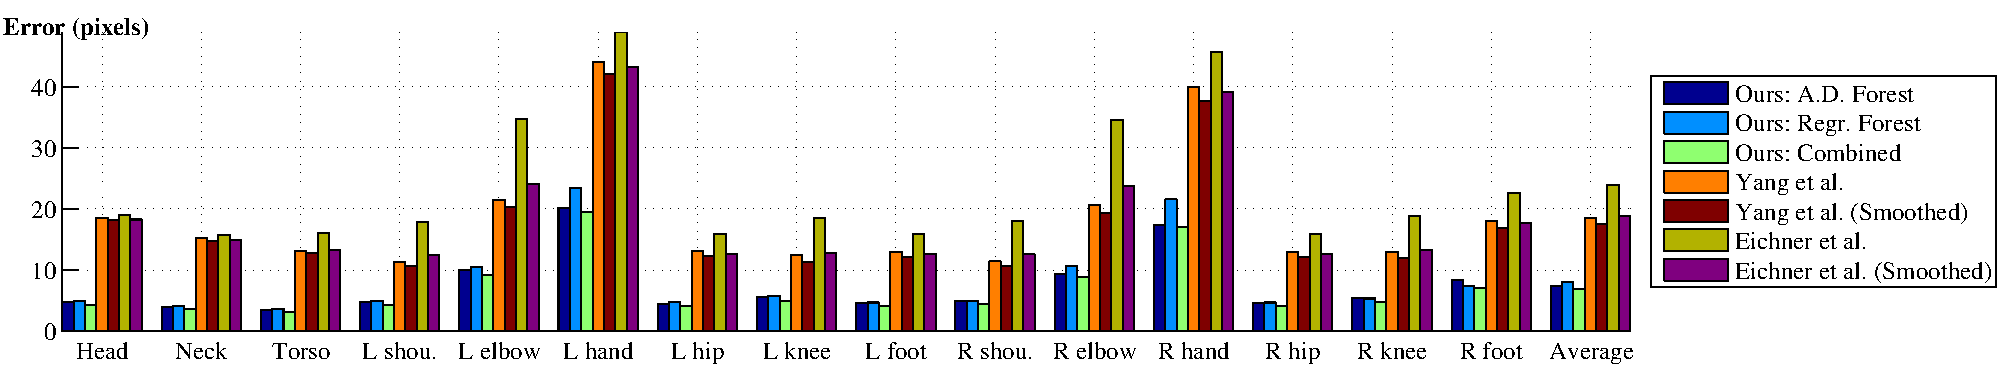
\includegraphics[width=1.02\linewidth]{fig/poseest/errplot2d.pdf} 
	%\vspace{-1mm} 
 	
\includegraphics[width=0.6\linewidth]{fig/poseest/plot_legend.pdf}
	\caption{2D joint localisation errors of our methods, \cite{Yang2011} and \cite{Eichner2012} their median smoothed versions.}
\label{fig:errorplot2d}
\end{figure*}


\section{Evaluation}
\subsection{The APE Evaluation Dataset}
Experiments were performed to investigate the feasibility of the proposed approach. 
Existing public 3D pose datasets are inadequate to justify the main objectives of the proposed approach. Whilst benchmarks such as \cite{Sigal2010, Yao2012} model joint angles rather than joint positions using sophisticated techniques, e.g. camera networks, from a static area, our framework focuses on flexible, multi-action 3D HPE from monocular videos without using background statistics.

To this end, we collected the \emph{action-pose-estimation (APE)} dataset for both quantitative and qualitative evaluations. The APE dataset contains $245$ sequences from $7$ subjects performing $7$ categories of actions. Videos of each subject were recorded in different environments, changing camera poses and moving background objects. The APE dataset will be made publicly available. 
%We refer the reader to \cite{APEwebsite} for details about the dataset.

The setting of APE dataset is considered challenging for traditional 3D HPE because: (1) no scene-dependent cues, \eg foreground segmentation, can be applied, (2) testing is done in unseen environments. 
Experiments are divided into two parts. In the first part, pose estimation accuracy was evaluated quantitatively with ground truth and current state-of-the-arts, in 3D and 2D respectively. In the second part, we demonstrated the knowledge transfer ability qualitatively, by testing with other videos and datasets.     


\subsection{Experimental Results}

\begin{figure}[*ht]
\centering
	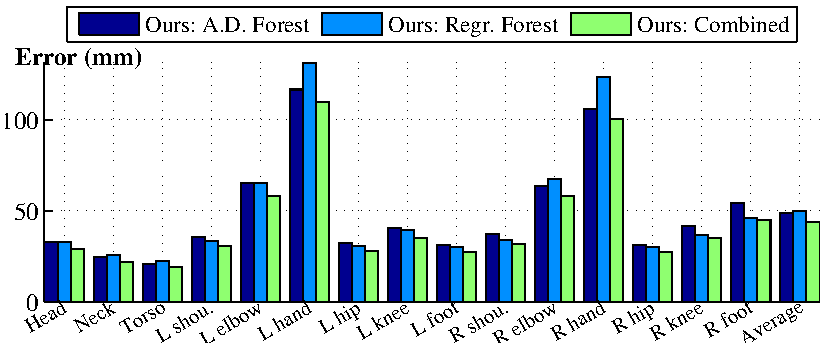
\includegraphics[width=1\linewidth]{fig/poseest/errplot3d.pdf} 
	\caption{3D joint localisation errors based on ground truth pose from Kinect sensor}
\label{fig:errorplot3d}
\end{figure}



\begin{figure}
	\centering
	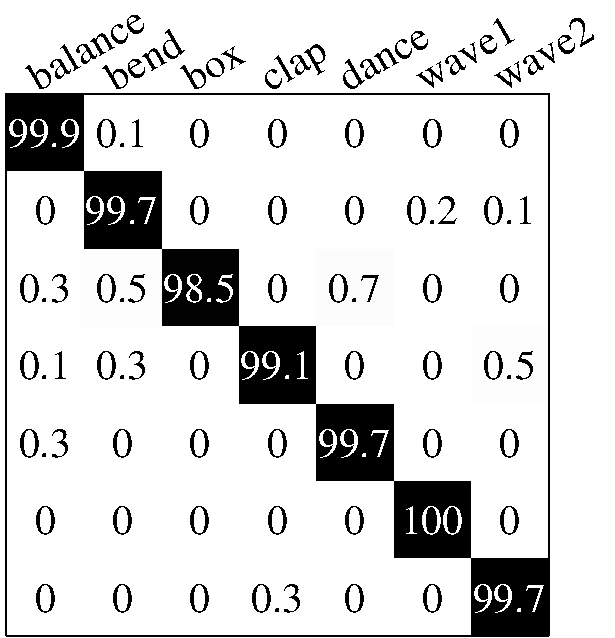
\includegraphics[height=0.30\linewidth]{fig/poseest/confm_detection.pdf} \hspace{1cm}
	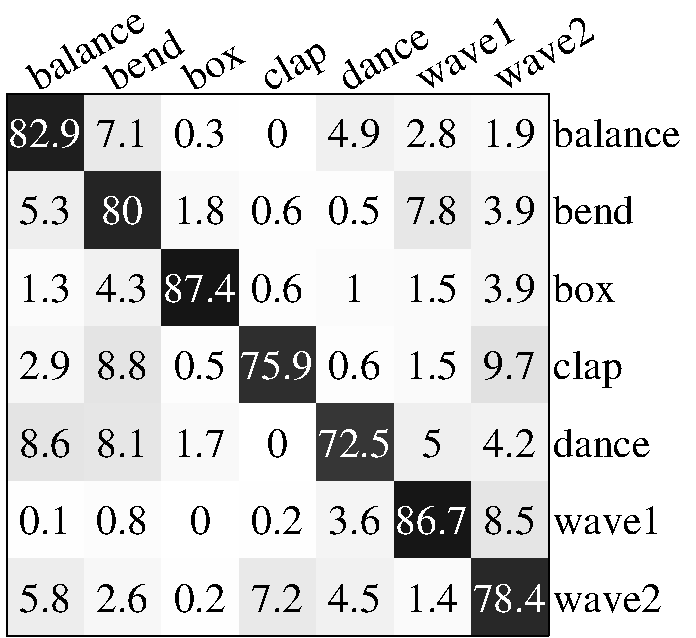
\includegraphics[height=0.30\linewidth]{fig/poseest/confm_regression.pdf}
	\caption{Confusion matrices of action classification by (left) action detection forest, and (right) cross-modality regression forest} 
	\label{fig:confm}
\end{figure}

\paragraph{Quantitative Evaluation.}
\label{sec:quant}
The proposed approach was evaluated quantitatively using the leave-one-out cross-validation strategy. A subject was taken out in turn for testing, thus the model is trained with $210$ sequences and the remaining $35$ sequences are evaluated. 
Snippets are extracted densely from training and testing data, where $\snippetlen = 10$. 
Table \ref{tab:rf_train_params} lists the training parameters. 
%Parameters used in training are shown in table \ref{tab:rf_train_params}. 

\begin{table}
	\centering
	{\footnotesize
	\begin{tabular}{|c|c|c|c|}
		\hline 
		Forest & \# tree & Max. depth & Min. node size \\ \hline 
		$\forestd$ & 10 & 16 & 15 \\ \hline 
		$\forestr$ & 10 & 14 & 20 \\ \hline 
	\end{tabular} 
	\caption{Parameters used in training $\forestd$ and $\forestr$.}
	\label{tab:rf_train_params}
}
\end{table}

\begin{table}[ht]
\centering
{\footnotesize
\begin{minipage}[b]{1\linewidth} 
\centering
\begin{tabular}{|p{2.5cm}|@{\,}c@{\,}|@{\,}c@{\,}|@{\,}c@{\,}|@{\,}c@{\,}|@{\,}c@{\,}|@{\,}c@{\,}|@{\,}c@{\,}|}
\hline
\textbf{Method} /  \textbf{Action} / \textbf{Error (mm)}& 
\raisebox{-4mm}{\rotatebox{90}{\textbf{Balance}}}
& 
\raisebox{-4mm}{\rotatebox{90}{\textbf{Bend}}}
& 
\raisebox{-4mm}{\rotatebox{90}{\textbf{Box}}}		
& 
\raisebox{-4mm}{\rotatebox{90}{\textbf{Clap}}}	
&
\raisebox{-4mm}{\rotatebox{90}{\textbf{Dance}}}
& 
\raisebox{-4mm}{\rotatebox{90}{\textbf{Wave 1}}}
& 
\raisebox{-4mm}{\rotatebox{90}{\textbf{Wave 2}}} 
\\ 
\hline
\hline
\textbf{Ours:A. D. Forest}  	& 41.9 			& \textbf{58.6} & 84.3 			& 49.1 			& 47.4 			& 36.7 			& 36.2 \\ 
\textbf{Ours:Regr. Forest}  	& 41.4 			& 69.7 			& \textbf{60.3} & 52.2 			& 58.2 			& 36.1 			& 39.1 \\ 
\textbf{Ours:Combined} 			& \textbf{37.8} & 58.8 			& 66.2 			& \textbf{41.0} & \textbf{45.1} & \textbf{30.1} & \textbf{34.6}\\  
\hline
\end{tabular}
\captionof{table}{Per-class joint localisation accuracy (3D)} 
\label{tab:errperclass3D}
\end{minipage}
\begin{minipage}[b]{1\linewidth} 
\centering
\begin{tabular}{|p{2.5cm}|@{\,}c@{\,}|@{\,}c@{\,}|@{\,}c@{\,}|@{\,}c@{\,}|@{\,}c@{\,}|@{\,}c@{\,}|@{\,}c@{\,}|}
\hline
\hline
\textbf{Method} /  \textbf{Action} / \textbf{Error (pixel)}& 
\raisebox{-4mm}{\rotatebox{90}{\textbf{Balance}}}
& 
\raisebox{-4mm}{\rotatebox{90}{\textbf{Bend}}}
& 
\raisebox{-4mm}{\rotatebox{90}{\textbf{Box}}}		
& 
\raisebox{-4mm}{\rotatebox{90}{\textbf{Clap}}}	
&
\raisebox{-4mm}{\rotatebox{90}{\textbf{Dance}}}
& 
\raisebox{-4mm}{\rotatebox{90}{\textbf{Wave 1}}}
& 
\raisebox{-4mm}{\rotatebox{90}{\textbf{Wave 2}}} \\ 
\hline
\textbf{Ours:A. D. Forest}  	& 6.1 			& \textbf{10.2} & 13.1 			& 6.6 			& 7.3 			& 6.7 			& 5.1 \\ 
\textbf{Ours:Regr. Forest}  	& 6.6 			& 13.1 			& \textbf{9.7} 	& 6.4 			& 8.9 			& 6.4 			& 6.4 \\ 
\textbf{Ours:Combined} 			& \textbf{5.6} 	& 10.7 			& 10.4 			& \textbf{5.4} 	& \textbf{7.0} 	& \textbf{4.8} & \textbf{5.2}\\ 
\hline
\textbf{Eichner et al.\cite{Eichner2012}}  	& 20.6 			& 28.6 			& 26.4 			& 22.5 			& 22.6 			& 22.3 			& 24.8 \\ 
\textbf{Yang et al. \cite{Yang2011}}  	& 14.2 			& 23.7 			& 21.6 			& 17.1 			& 16.7 			& 16.5 			& 19.3 \\ 
\hline
\end{tabular}
\captionof{table}{Per-class joint localisation accuracy (2D)} 
\label{tab:errperclass2D}
\end{minipage}
}
\end{table}


Pose estimation accuracy was evaluated in both 2D and 3D. Accuracies of 3D joint coordinates were compared directly with ground truth 3D poses captured by the Kinect sensor. Accuracies in 2D were measured by back-projecting the poses to image coordinates.  
Besides the combined pose estimation $\finalpose$, we also evaluated each of the forests alone, and compared it with the latest 2D HPE algorithms \cite{Eichner2012} and \cite{Yang2011}. 
In order to cope with actions performed in different speeds, testing videos are preprocessed by normalising with respect to their action speeds estimated from the first $25$ frames of the videos.
In order to make a fair comparison, the joint coordinates from the frame-based algorithms \cite{Eichner2012} and \cite{Yang2011} are temporally smoothed by a $10$-frame median filter, as our approach estimates poses from multiple-frame snippets. 

Action classification rates of individual frames by both forests are presented in figure \ref{fig:confm}. 
The action detection forest achieves excellent accuracy, as it has been optimised for classification during learning, the video-based input, snippet, also provides temporal cues that improve classification. It complements the regression forests that focus on the localisation accuracy of joints.    
The average 3D joint localisation errors of the experiments were reported in figure \ref{fig:errorplot3d}. 
Sample results of the proposed method are also presented in figure \ref{fig:aperesults}\footnote{Please refer to the supplementary materials for more results.}. 

The comparison our method and other 2D HPE algorithms is illustrated in figure \ref{fig:errorplot2d}.
The proposed framework showed promising results, by extending the flexibility of \cite{Yang2011}, the proposed method showed high robustness in 3D pose estimation and outperformed both state-of-the-arts in the 2D tests. The hand parts have the highest localisation errors because of their large movements and frequent occlusions, which are also indicated by the big variance ellipsoids in figure \ref{fig:aperesults}.

The per-class localisation errors are listed in table \ref{tab:errperclass3D} (3D) and \ref{tab:errperclass2D} (2D). While some classes reported significant improvements after combining the results of action detection and pose regression, \eg ``clap'' and ``wave 1'', the ``bend'' and ``box'' class reported the highest error rates.
The 2D part detections obtained from the ``box'' and ``bend'' classes are less accurate than those from other classes.  For the ``box'' action, self-occlusion happens frequently such that the part detector is confused about the left and right hand positions, making the hand position distributions spread around the torso as in figure \ref{fig:aperesults}(p). 
Similarly, when the arms are stretched overhead and occluded, the 2D DPM model used in the experiments gives incorrect results.  

% classnames = {'wave2','balance','bend','box','clap','dance','wave1'};
\begin{figure*}[*th] 
\begin{center}
{\footnotesize
\begin{tabular}{@{}c@{}c@{}c@{}c@{}c@{}c@{}c@{}c@{}} 
\rotatebox{90}{\hspace{3mm}\textbf{(a) Balance}}
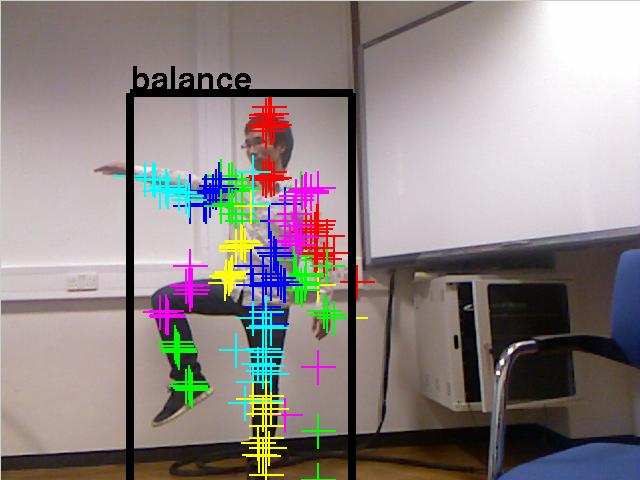
\includegraphics[height=0.11\linewidth]{fig/poseest/APE/balc.jpg} 
&
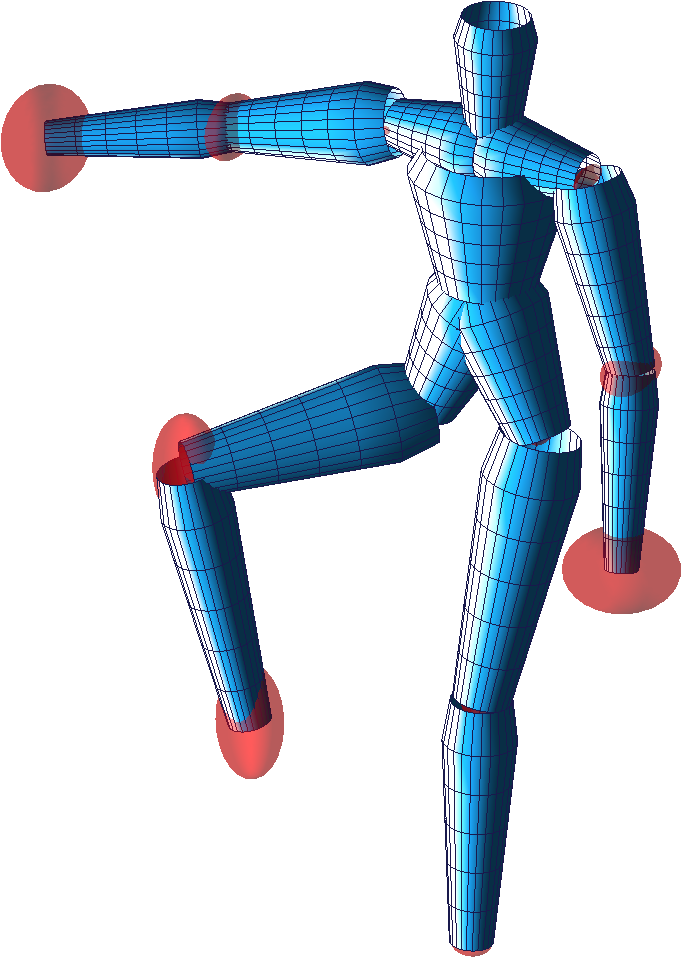
\includegraphics[height=0.135\linewidth]{fig/poseest/APE/balc.png}
& 
\rotatebox{90}{\hspace{3mm}\textbf{(b) Balance}}
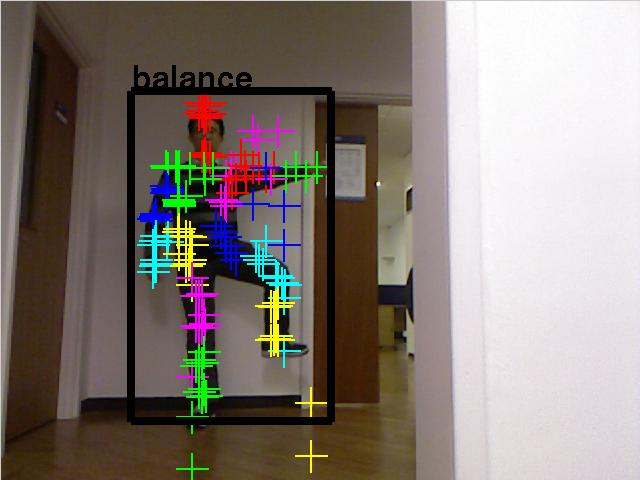
\includegraphics[height=0.11\linewidth]{fig/poseest/APE/balc2.jpg} 
&
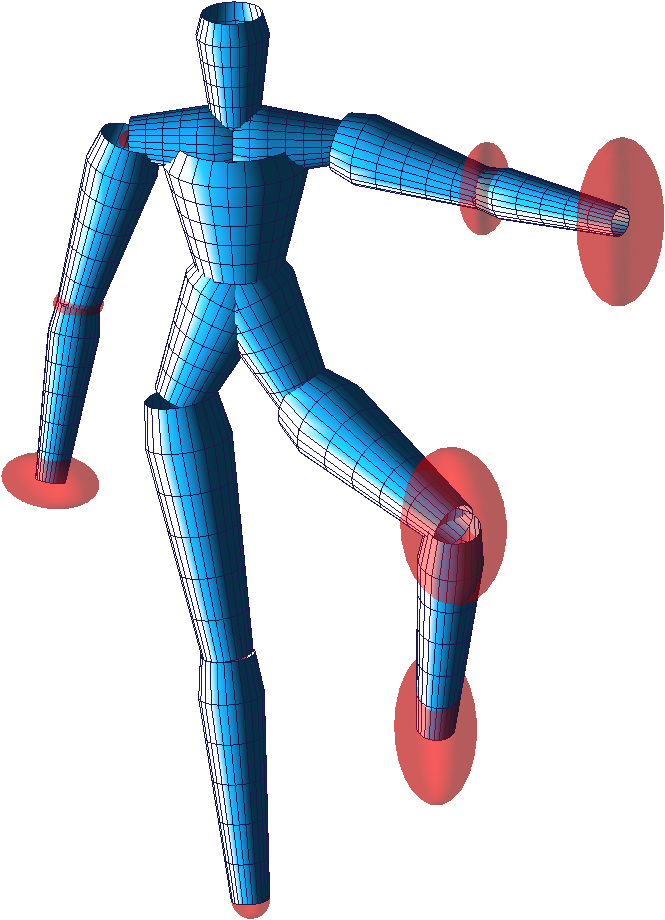
\includegraphics[height=0.135\linewidth]{fig/poseest/APE/balc2.png}
& 
\rotatebox{90}{\hspace{3mm}\textbf{(c) Bend}}
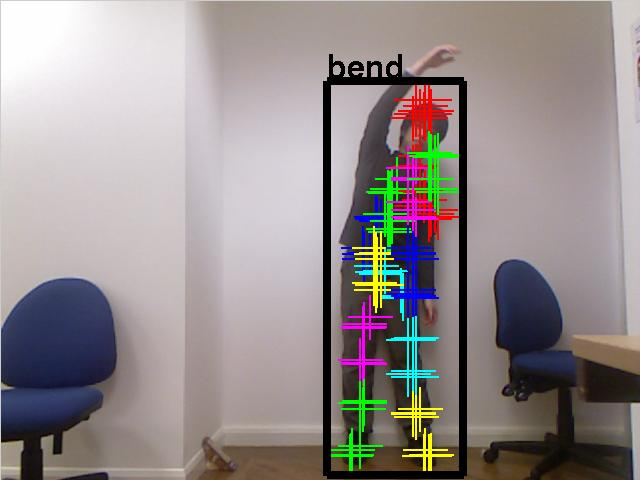
\includegraphics[height=0.11\linewidth]{fig/poseest/APE/bend.jpg} 
&
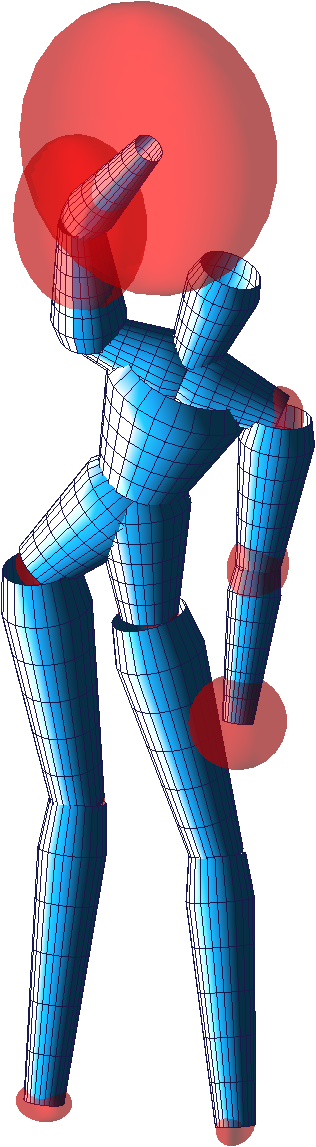
\includegraphics[height=0.135\linewidth]{fig/poseest/APE/bend.png}
& 
\rotatebox{90}{\hspace{3mm}\textbf{(d) Bend}}
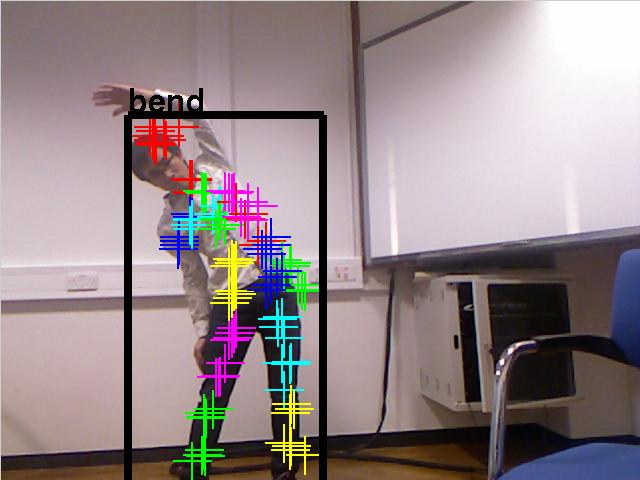
\includegraphics[height=0.11\linewidth]{fig/poseest/APE/bend2.jpg} 
&
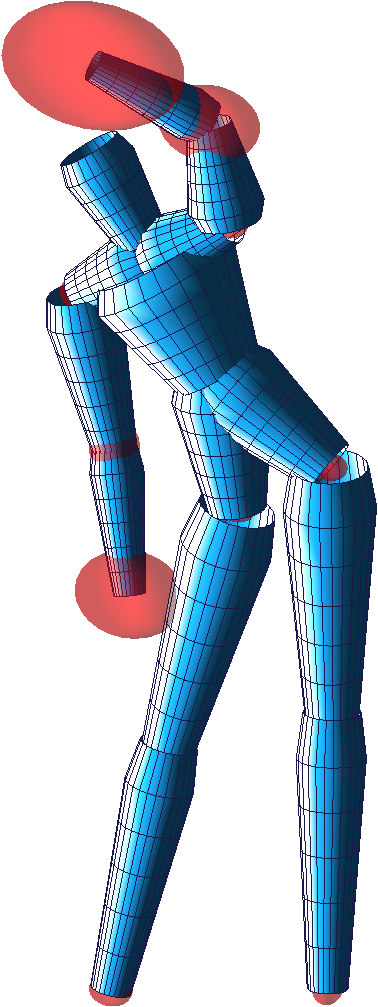
\includegraphics[height=0.135\linewidth]{fig/poseest/APE/bend2.png}
\\
\rotatebox{90}{\hspace{3mm}\textbf{(e) Box}}
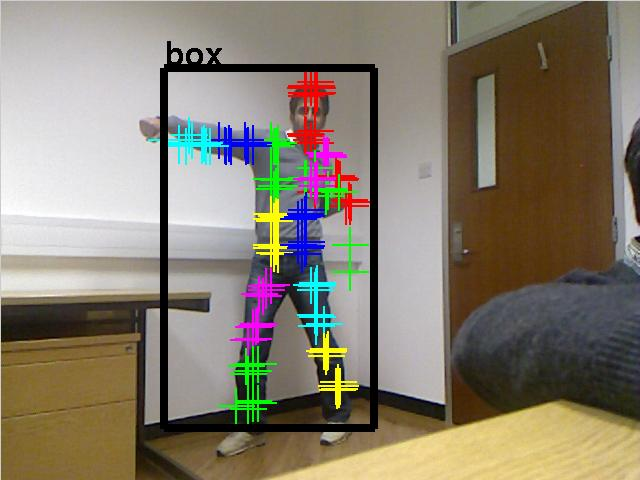
\includegraphics[height=0.11\linewidth]{fig/poseest/APE/boxx.jpg} 
&
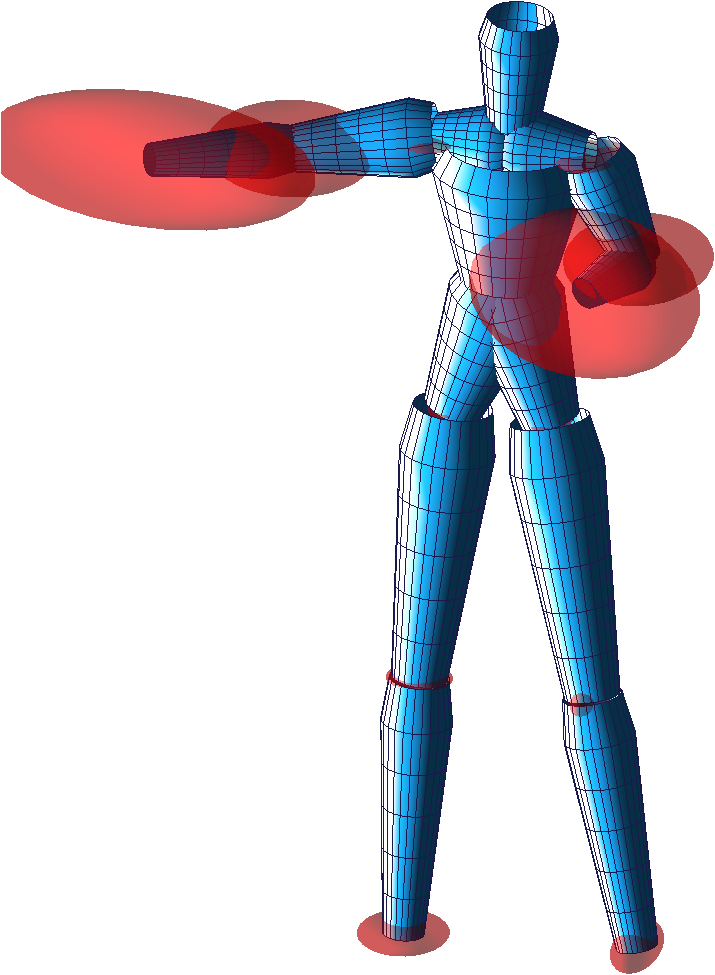
\includegraphics[height=0.135\linewidth]{fig/poseest/APE/boxx.png}
& 
\rotatebox{90}{\hspace{3mm}\textbf{(f) Box}}
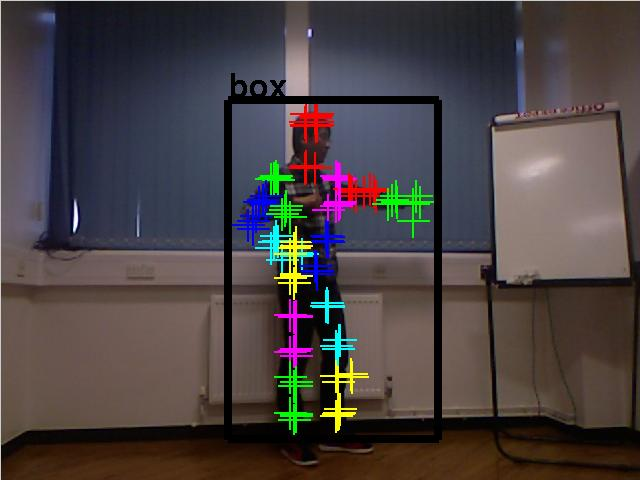
\includegraphics[height=0.11\linewidth]{fig/poseest/APE/boxx2.jpg} 
&
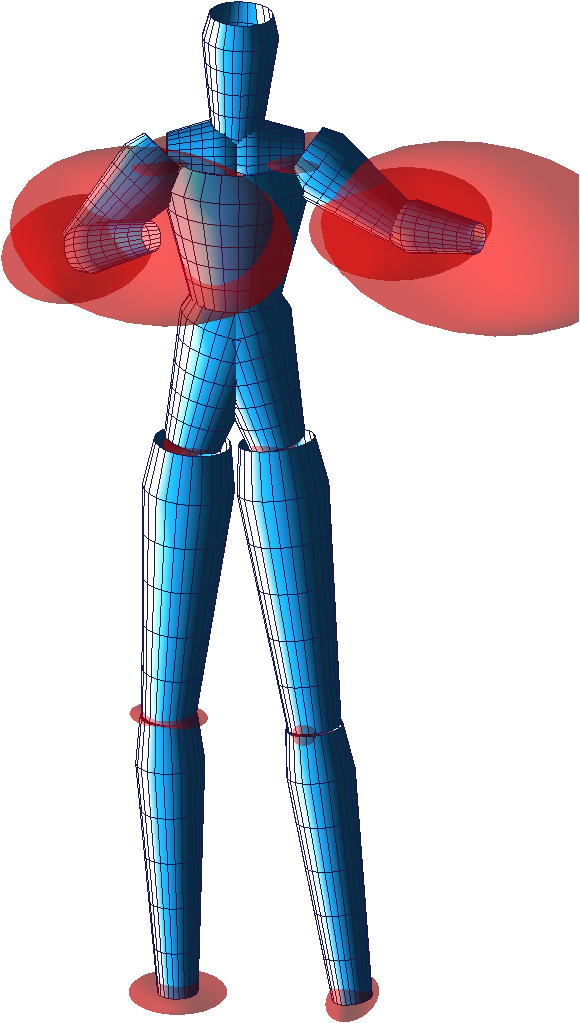
\includegraphics[height=0.135\linewidth]{fig/poseest/APE/boxx2.png}
& 
\rotatebox{90}{\hspace{3mm}\textbf{(g) Clap}}
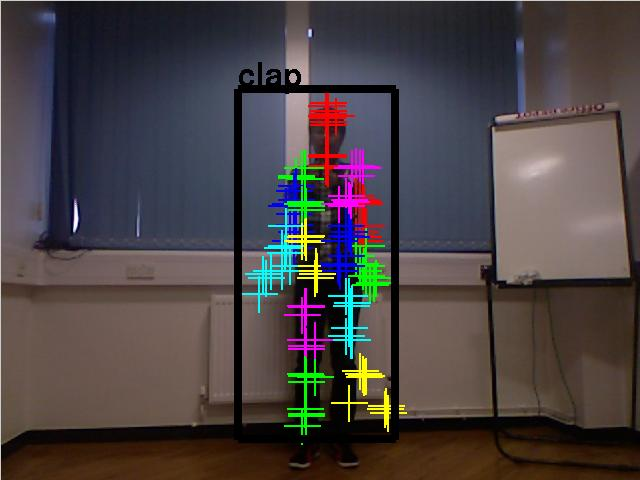
\includegraphics[height=0.11\linewidth]{fig/poseest/APE/clap.jpg} 
&
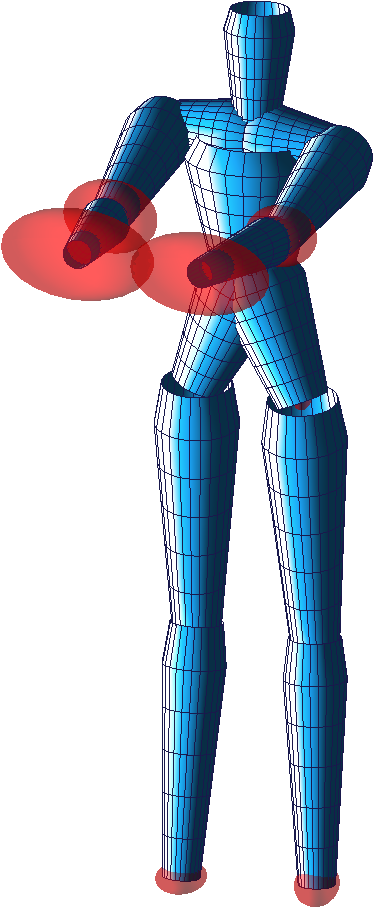
\includegraphics[height=0.135\linewidth]{fig/poseest/APE/clap.png}
& 
\rotatebox{90}{\hspace{3mm}\textbf{(h) Clap}}
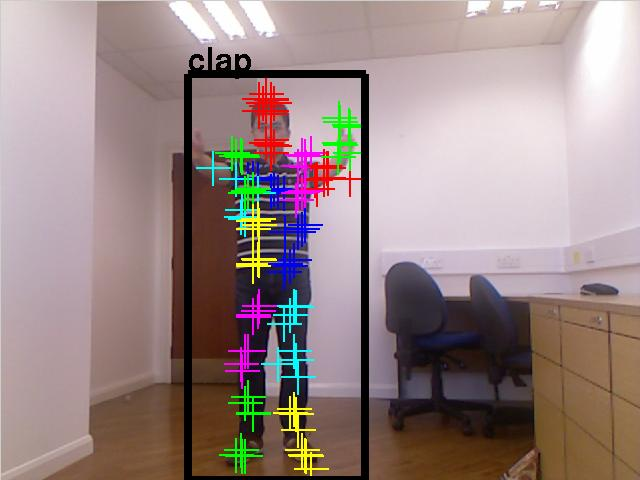
\includegraphics[height=0.11\linewidth]{fig/poseest/APE/clap2.jpg} 
&
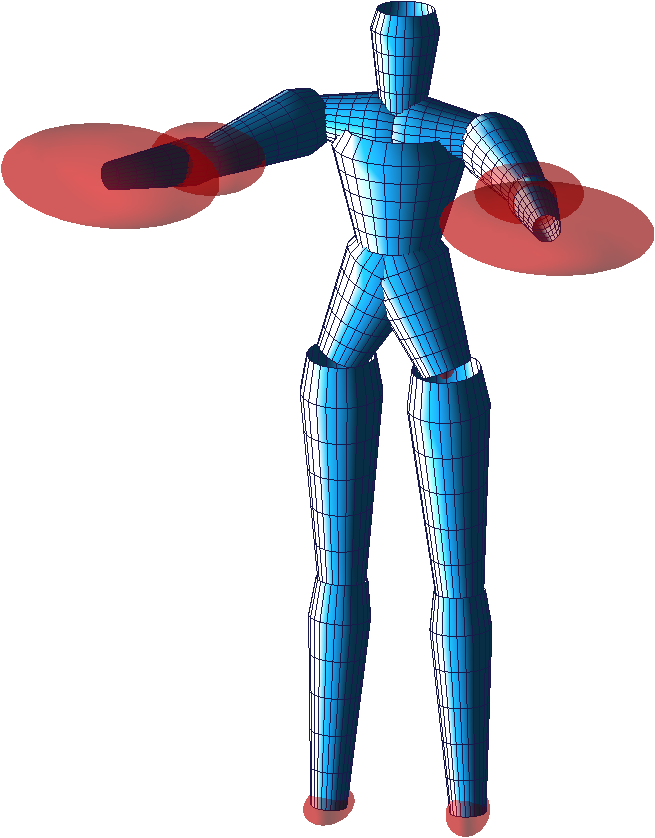
\includegraphics[height=0.135\linewidth]{fig/poseest/APE/clap2.png}
\\
\rotatebox{90}{\hspace{3mm}\textbf{(i) Dance}}
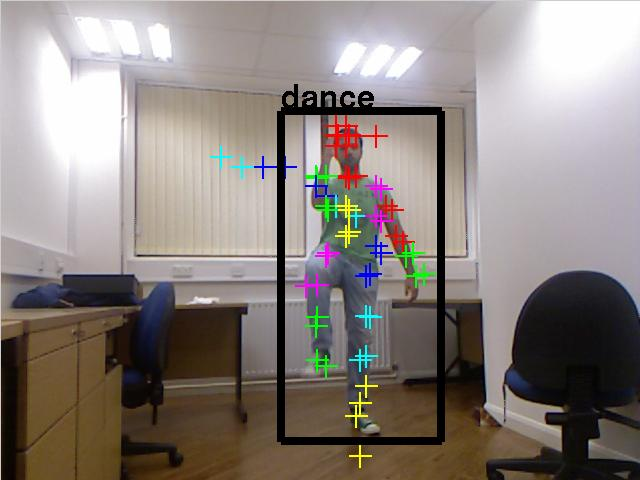
\includegraphics[height=0.11\linewidth]{fig/poseest/APE/dance.jpg} 
&
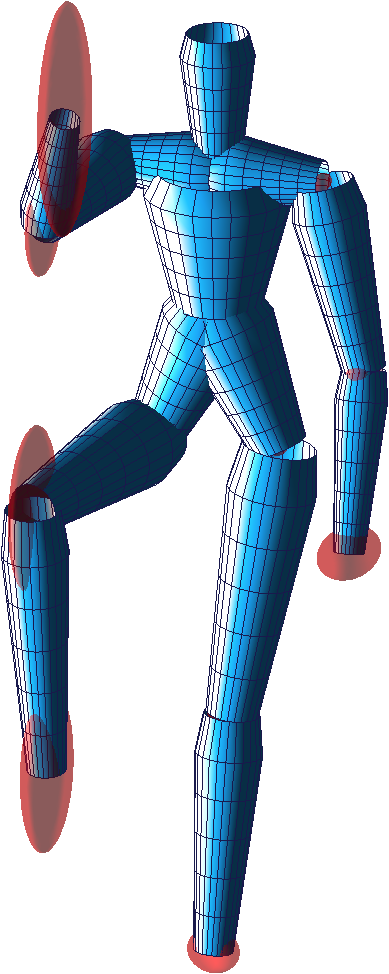
\includegraphics[height=0.135\linewidth]{fig/poseest/APE/dance.png}
& 
\rotatebox{90}{\hspace{3mm}\textbf{(j) Dance}}
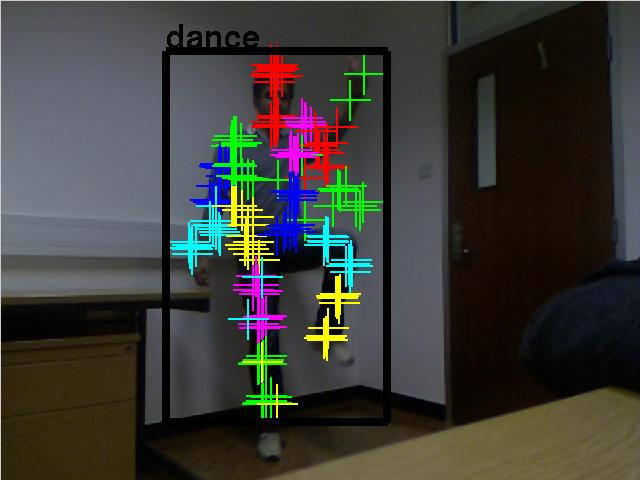
\includegraphics[height=0.11\linewidth]{fig/poseest/APE/dance2.jpg} 
&
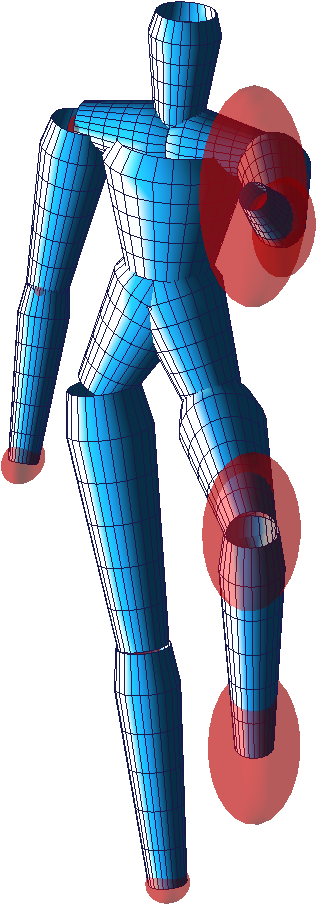
\includegraphics[height=0.135\linewidth]{fig/poseest/APE/dance2.png}
& 
\rotatebox{90}{\hspace{3mm}\textbf{(k) Wave 1}}
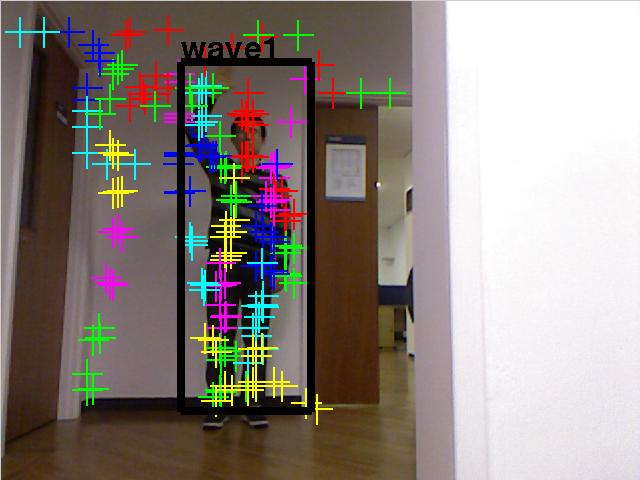
\includegraphics[height=0.11\linewidth]{fig/poseest/APE/wave1.jpg} 
&
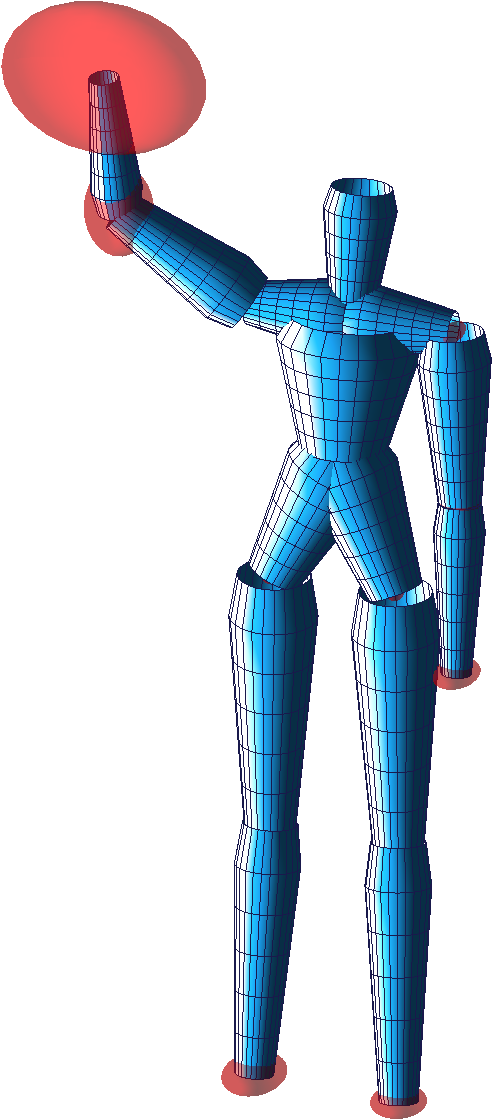
\includegraphics[height=0.135\linewidth]{fig/poseest/APE/wave1.png}
& 
\rotatebox{90}{\hspace{3mm}\textbf{(l) Wave 1}}
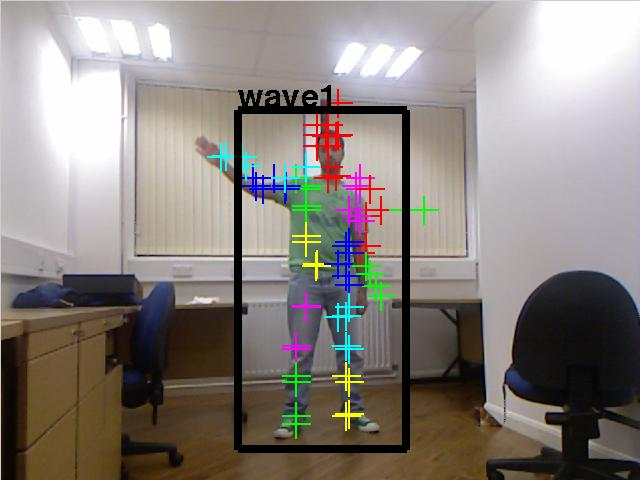
\includegraphics[height=0.11\linewidth]{fig/poseest/APE/wave12.jpg} 
&
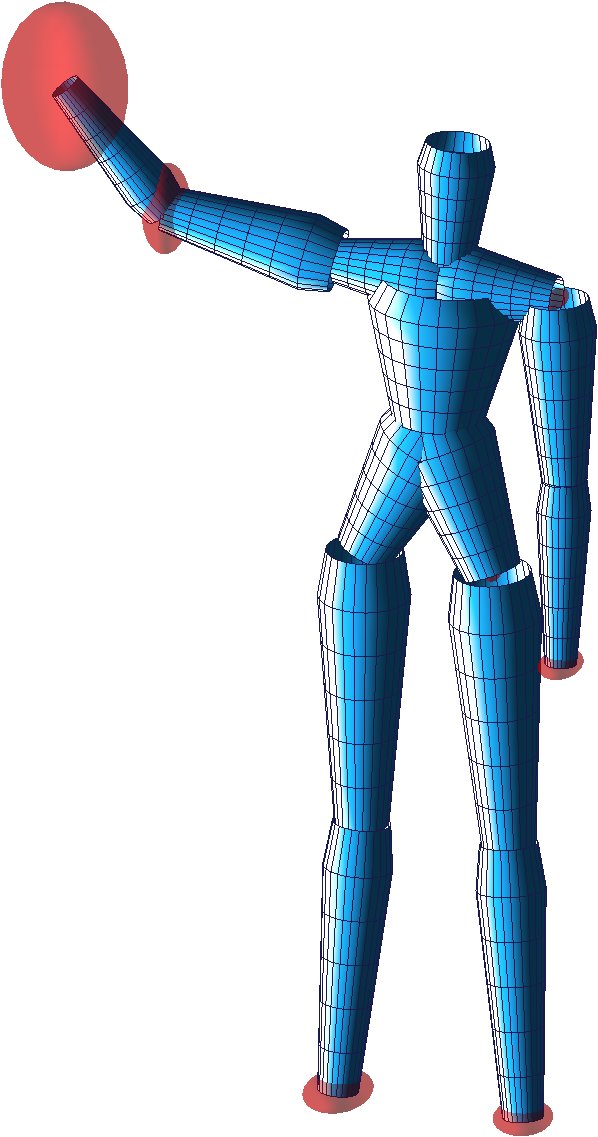
\includegraphics[height=0.135\linewidth]{fig/poseest/APE/wave12.png}
\\
\rotatebox{90}{\hspace{3mm}\textbf{(m) Wave 2}}
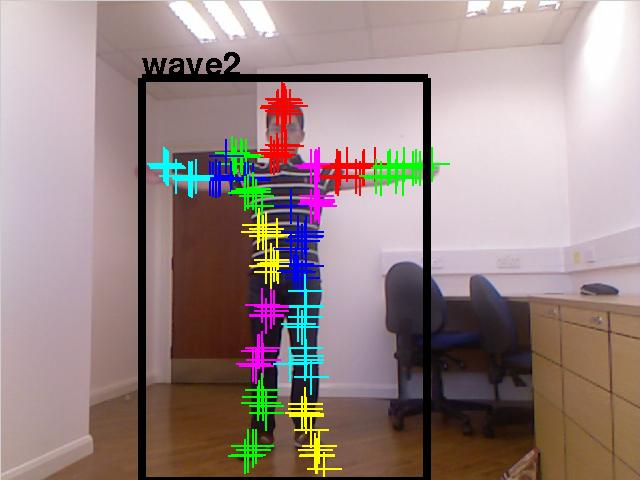
\includegraphics[height=0.11\linewidth]{fig/poseest/APE/wave2.jpg} 
&
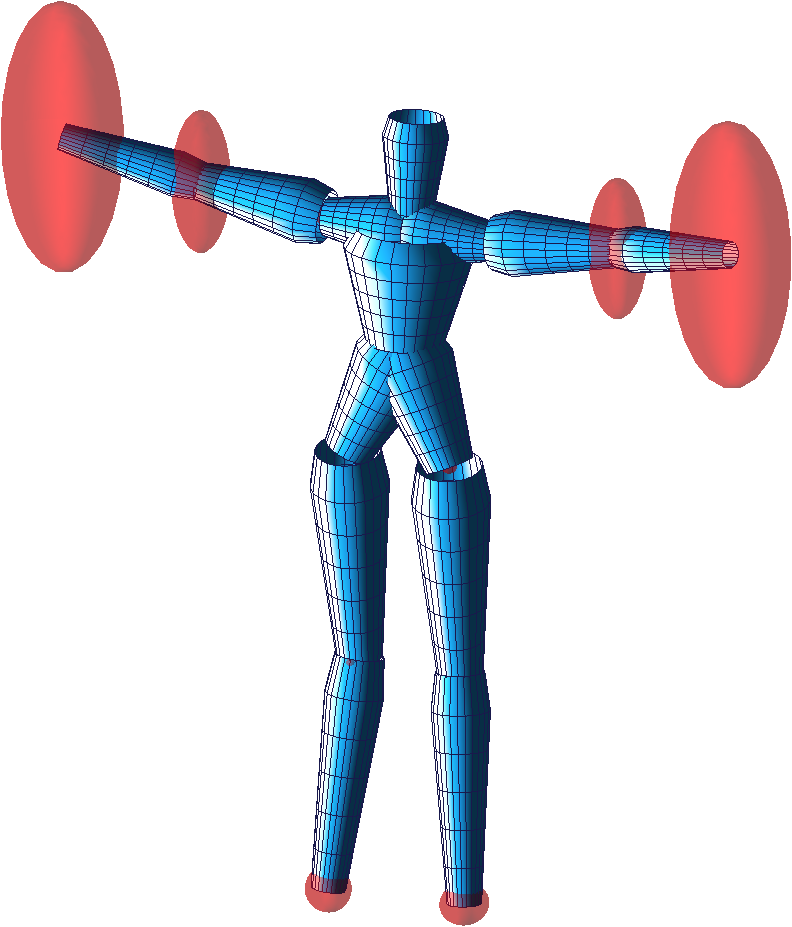
\includegraphics[height=0.135\linewidth]{fig/poseest/APE/wave2.png}
& 
\rotatebox{90}{\hspace{3mm}\textbf{(n) Wave 2}}
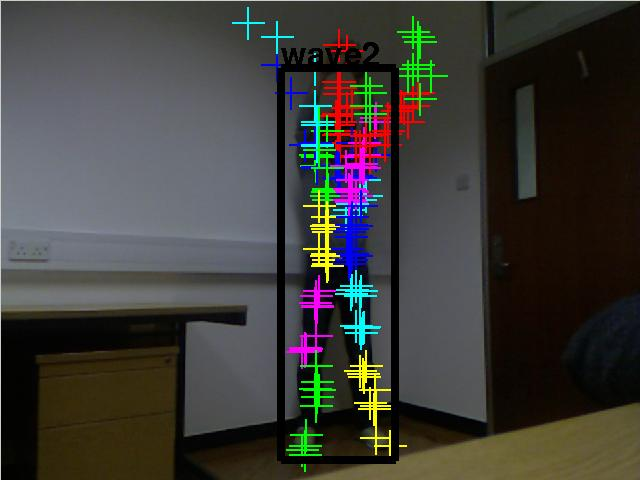
\includegraphics[height=0.11\linewidth]{fig/poseest/APE/wave22.jpg} 
&
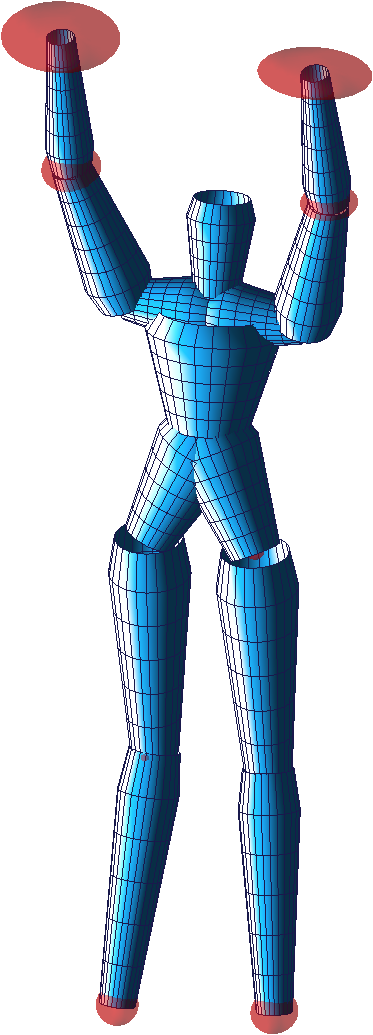
\includegraphics[height=0.135\linewidth]{fig/poseest/APE/wave22.png}
& 
\rotatebox{90}{\hspace{3mm}\textbf{(o) Bend}}
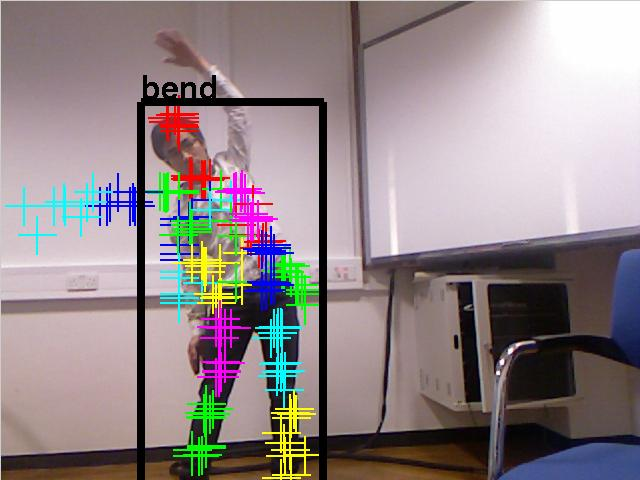
\includegraphics[height=0.11\linewidth]{fig/poseest/APE/benderr.jpg} 
&
\includegraphics[height=0.135\linewidth]{fig/poseest/APE/benderr.png}
& 
\rotatebox{90}{\hspace{3mm}\textbf{(p) Box}}
\includegraphics[height=0.11\linewidth]{fig/poseest/APE/boxxerr.jpg} 
&
\includegraphics[height=0.135\linewidth]{fig/poseest/APE/boxxerr.png}

\end{tabular}
\caption{3D pose estimation results with different action classes from the APE dataset: (left) Detected 2D parts and bounding box from action detection (right) the 3D pose estimated.  Red ellipsoids represent the confidence region of pose estimation, $\finalvariance$, in equation (\ref{eq:combination2}). Sample (o) and (p) shows the wrong pose estimations when the 2D body part detector fails.}
\label{fig:aperesults}
} 
\end{center} 
\end{figure*} 


\paragraph{Qualitative Evaluation.}
Knowledge transfer was evaluated by reusing the models trained in section \ref{sec:quant} to other datasets without retraining.
The KTH \cite{Schuldt2004} and Weizmann \cite{Gorelick2007} dataset 
were used in the experiments as they shared action categories with the APE dataset. 

The experimental results are reported qualitatively in figure \ref{fig:otherresults}. Even though the input videos are of extremely low resolutions, rendering them inapplicable to typical 3D HPE methods, our framework is still able to estimate their actions and poses simultaneously with encouraging accuracy. 
Incorrect poses were estimated when too many false positive parts are detected from the low resolution images, \eg figure \ref{fig:otherresults}(g--h). 


\paragraph{Discussion.}
The experimental results have demonstrated high feasibility in the idea of using action detection to estimate 3D poses under challenging conditions.  
Coupling the outputs from the random forests, the 3D pose estimation accuracy is further enhanced. Action detection gives a global pose estimation and the corresponding class label. Meanwhile, errors in the initial global estimation, due to the differences among individual action patterns, are corrected locally by regression forests, which improves the accuracy of the final pose estimation as shown in figure \ref{fig:errorplot3d}. 

On the other side, there is still room for improvement in the proposed approach. The proposed method relies on DPM as the only source of input. Albeit great flexibility, \cf \cite{Yang2011}, the performance of a DPM depends on its training data. Our method handles minor errors gracefully by allowing multiple hypotheses and snippet-based input, but large errors cannot be recovered completely, \eg figure \ref{fig:aperesults}(o) and \ref{fig:aperesults}(p) for APE dataset, and \ref{fig:otherresults}(g) and \ref{fig:otherresults}(h) for KTH and Weizmann dataset respectively. 
Besides, the proposed method runs at $0.31$fps. Feature extraction from DPM is the run-time bottleneck. The pose estimatior alone runs at about $5$fps by precomputing the DPM features. 

\begin{figure*}[th] 
\begin{center}
{\footnotesize
\begin{tabular}{@{}c@{}c@{}c@{}c@{}c@{}c@{}c@{}c@{}} 
\rotatebox{90}{\hspace{3mm}\textbf{(a) Wave 2 }}
\includegraphics[height=0.11\linewidth]{fig/poseest/others/kth3.jpg} 
&
\includegraphics[height=0.135\linewidth]{fig/poseest/others/kth3.png}
& 
\rotatebox{90}{\hspace{3mm}\textbf{(b) Wave 2 }}
\includegraphics[height=0.11\linewidth]{fig/poseest/others/kth1.jpg} 
&
\includegraphics[height=0.135\linewidth]{fig/poseest/others/kth1.png}
& 
\rotatebox{90}{\hspace{3mm}\textbf{(c) Clap }}
\includegraphics[height=0.11\linewidth]{fig/poseest/others/kth2.jpg} 
&
\includegraphics[height=0.135\linewidth]{fig/poseest/others/kth2.png}
& 
\rotatebox{90}{\hspace{3mm}\textbf{(d) Wave 1 }}
\includegraphics[height=0.11\linewidth]{fig/poseest/others/weiz3.jpg} 
&
\includegraphics[height=0.135\linewidth]{fig/poseest/others/weiz3.png}
\\
\rotatebox{90}{\hspace{3mm}\textbf{(e) Wave 1 }}
\includegraphics[height=0.11\linewidth]{fig/poseest/others/weiz1.jpg} 
&
\includegraphics[height=0.135\linewidth]{fig/poseest/others/weiz1.png}
& 
\rotatebox{90}{\hspace{3mm}\textbf{(f) Wave 2 }}
\includegraphics[height=0.11\linewidth]{fig/poseest/others/weiz2.jpg} 
&
\includegraphics[height=0.135\linewidth]{fig/poseest/others/weiz2.png}
& 
\rotatebox{90}{\hspace{3mm}\textbf{(g) Wave 2 }}
\includegraphics[height=0.11\linewidth]{fig/poseest/others/ktherr.jpg} 
&
\includegraphics[height=0.135\linewidth]{fig/poseest/others/ktherr.png}
& 
\rotatebox{90}{\hspace{3mm}\textbf{(h) Wave 1 }}
\includegraphics[height=0.11\linewidth]{fig/poseest/others/weizerr.jpg} 
&
\includegraphics[height=0.135\linewidth]{fig/poseest/others/weizerr.png}
\end{tabular}
\caption{Sample results obtained from applying the same model trained in Section \ref{sec:quant} to KTH (a--c, g) and Weizmann dataset (d--f, h).} 
\label{fig:otherresults}
} 
\end{center} 
\end{figure*} 


\section{Conclusions}
\label{sec:conclusions}

The challenging problem of 3D human pose estimation is discussed in this paper. 
While traditional methods for 3D human pose estimation emphasise accuracy over their compatibility with realistic applications, we present a novel practical approach without using any scene-dependent constraints.
We investigate the new area of using action for pose estimation. The proposed method combines human action detection and deformable part model-based 2D human pose estimation to estimate 3D poses from unconstrained, monocular videos.  
The new APE dataset is introduced to evaluate the feasibility of our approach.  
Experimental results have shown promising results and also high flexibility by transferring the knowledge obtained from training data to other unseen datasets.
In the future we plan to apply kinematic constraints in our system for pose refinement. 
We suggest that the collaboration between the techniques in human action and pose analysis will be beneficial to both areas of computer vision research in the coming future.  


\chapter{Future Work: 3-D Hand Pose Estimation from Depth Sensors}

\section{Introduction}
%Articulated hand pose estimation has been a longstanding challenge in computer vision. 
%It is essential to various applications including user human-computer interaction, graphics and activity analysis.
%It shares a lot of similarities with the popular 3-D body pose estimation. 
Articulated hand pose estimation shares a lot of similarities with the popular 3-D body pose estimation. 
Both tasks aim to recognise the configuration of an articulated subject with a high degree of freedom. 
%They also require domain knowledge, \eg kinematics \cite{Gorce_PAMI_11} or actions \cite{Yu_CVPR_13}, in order to infer articulated poses from limited input data. 
While latest depth sensor technologies has enabled body pose estimation in real-time \cite{Baak_ICCV_11, Shotton_CVPR_11, Girshick_ICCV_11, Sun_CVPR_12}, hand pose estimation still remains unresolved.
Despite their similarities, proven approaches in body pose estimation cannot be repurposed directly to hand articulations, due to the unique challenges of the task:   \\
\textbf{(1) Occlusions and viewpoint changes.} Self occlusions are prevalent in hand articulations. %The complex anatomy of human hand provides at least 26 degrees of freedom. 
Compared with limbs in body pose, fingers perform more sophisticated articulations. 
%In addition, d
Different from body poses which are usually upright and frontal \cite{Eichner_IJCV_12}, different viewpoints can render different depth images despite the same hand articulation. \\  
\textbf{(2) Noisy hand pose data.} Body poses usually occupy larger and relatively static regions in the depth images. 
Hands, however, are often captured in a lower resolution.
%, which lead to more noisy inputs than that of body poses 
As shown in Fig. \ref{fig:intro}, missing parts and quantisation error is common in hand pose data, especially at small, partially occluded parts such as finger tips. 
%Regardless of the object distance, missing values are created when a complete structured light patterns fail to project on the occlusion boundaries. 
Unlike sensor noise and depth errors in \cite{Girshick_ICCV_11} and \cite{Baak_ICCV_11}, these artifacts cannot be repaired or smoothed easily. Consequently, a large discrepancy is observed between synthetic and realistic data. 

Moreover, 
%due to noise, occlusions and the inherent complex structure of human hand, 
manually labelled realistic data are extremely costly to obtain. Existing state-of-the-arts resort to synthetic data, \eg \cite{Keskin_ECCV_12}, or model-based optimisation, \eg \cite{Gorce_PAMI_11, Oikonomidis_CVPR_12}. Nonetheless, such solutions do not consider the realistic-synthetic discrepancies, their performances are hence affected. Besides, the noisy realistic data make joint detection difficult, whereas in synthetic data joint boundaries are always clean and accurate.

%Whilst handling shape variation is crucial for body pose estimation \cite{Shotton_CVPR_11}, shape variations of human hands are generally smaller than that of body shape.        

% hand shapes 
\begin{figure}
\centering
\begin{subfigure}[b]{0.30\linewidth}
	\centering
	\raisebox{-1mm}{\includegraphics[width=0.8\linewidth]{fig/fig1_rgb.png}}
	\caption{RGB}
\end{subfigure}
\begin{subfigure}[b]{0.22\linewidth}
	\centering
	\raisebox{-1mm}{\includegraphics[width=0.7\linewidth]{fig/fig1_a.png}}
	\caption{Labels}
\end{subfigure}
\begin{subfigure}[b]{0.22\linewidth}
	\centering
	\raisebox{-1mm}{\includegraphics[width=0.7\linewidth]{fig/fig1_c.png}}
	\caption{Synthetic}
\end{subfigure}
\begin{subfigure}[b]{0.22\linewidth}
	\centering
	\raisebox{-2mm}{\includegraphics[width=0.8\linewidth]{fig/fig1_b.png}}
	\caption{Realistic}
\end{subfigure}
\caption{The ring finger is missing due to occlusions in (d), and the little finger is wider than the synthetic image in (c).}
\label{fig:intro}
\end{figure}

In this work, 
addressing the above challenges, 
we present a novel \emph{Semi-supervised Transductive Regression} (\STR) forest
%to address the above challenges
, by learning the relationship between realistic and synthetic data. 
This process is known as \emph{transductive transfer learning} \cite{Pan_TKDE_10}:   
A transductive model learns from a \emph{source domain}, \eg synthetic data
%, during the training process.
; on the other hand, it applies \emph{knowledge transform} to a different but related \emph{target domain}, \eg realistic data, in the testing stage. 
The \STR\ forest is also semi-supervised, learning the noisy appearances of realistic data from both labelled and unlabelled datapoints. As a result, it benefits from the characteristics of both domain: The \STR\ forest not only captures a wide range of poses from synthetic data, it also achieves promising accuracy in challenging environments by learning from realistic data. 
%In addition to the proposed \STR\ forest, 
In addition, we design an efficient pseudo-kinematic joint refinement algorithm to 
handle occluded and noisy
%deal with the severe occlusion issue in hand
articulations. 
%The proposed method utilises both realistic and synthetically generated training data. 
% a brief decription of the characteristics of our method 

As far as we are aware, the proposed method is the first semi-supervised and transductive articulated hand pose estimation framework.  
The main contribution of our work is threefold:\\ 
\textbf{(1) Realistic-Synthetic fusion:} Considering the issue of noisy inputs, we proposed the first transductive learning algorithm for 3-D hand pose estimation that captures the characteristics of both realistic and synthetic data.\\
%realistic and synthetic data, improving robustness and pose coverage simultaneously. \\
\textbf{(2) Semi-supervised learning:} The proposed learning algorithm utilises both labelled and unlabelled data, improving estimation accuracy while keeping a low labelling cost.  \\
\textbf{(3) Data-driven pseudo-kinematics:} The limitation of traditional Hough forest\cite{Gall_CVPR_09} against occlusions is improved by learning a data-driven pseudo-kinematic algorithm.


\section{Related Work}

% different shape --- apperance based 
\begin{figure*}[ht]
	\hspace{-4mm}
	\includegraphics[width=1.03\linewidth]{fig/fig2.pdf}
	\caption{The proposed \STR\ learning model.}
	\label{fig:concept}
\end{figure*}

\noindent\textbf{Hand pose estimation} Earlier approaches for articulated hand pose estimation are diversified, such as coloured markers \cite{Chua_IVC_02}, probabilistic line matching \cite{Athitsos_CVPR_03}, multi-camera network \cite{Guan_CVPRW_06} and Bayesian filter with Chamfer matching \cite{Stenger_PAMI_06}. 
%For example, Chua \etal \cite{Chua_IVC_02} recognises hand poses from colored markers on hand to analyse hand articulations. Athitsos \etal \cite{Athitsos_CVPR_03} estimates articulated hand and viewpoint from a database using probabilistic line matching. Pose ambiguities of hand poses are resolved using multiple cameras in \cite{Guan_CVPRW_06}. Stenger \etal \cite{Stenger_PAMI_06} infer hand poses using a Bayesian filter based on Chamfer matching. 
We refer the reader to \cite{Erol_CVIU_07} for a detailed survey of earlier hand pose estimation algorithms. 

\emph{Model-based tracking} methods are popular among recent state-of-the-arts. Hypotheses are generated from a visual model, \eg a 3-D hand mesh. Hand poses are tracked by fitting the hypotheses to the test data. For example, De La Gorce \etal \cite{Gorce_PAMI_11} use a hand mesh with detailed simulated texture and lighting. Hamer \etal \cite{Hamer_ICCV_09} address strong occlusions using local trackers at separate hand segments. Ballan \etal \cite{Ballan_ECCV_12} infer finger articulations by detecting salient points.  
Oikonomidis \etal \cite{Oikonomidis_ICCV_11} estimate hand poses in real-time from RGB-D images using particle swarm optimisation. Model-based approaches inherently handle joint articulations and viewpoint changes. 
However, their performances depend on the previous pose estimations, output poses may drift away from groundtruth when error accumulates over time. 
%When tracking is eventually lost, the incorrect poses cannot be recovered without manual re-initialisation.   
%Most model-based methods do not consider shape variations of hands due to the additional complexity involved \cite{Erol_CVIU_07}, which jeopardises their accuracies in realistic applications. 

\emph{Discriminative} approaches learn a mapping from visual features to the target parameter space, such as joint labels \cite{Shotton_CVPR_11} or joint coordinates \cite{Girshick_ICCV_11}.  
Instead of using a predefined visual model, discriminative methods learn a pose estimator from a labelled training dataset. 
Although discriminative methods have proved successful in real-time body pose estimation from depth sensors \cite{Shotton_CVPR_11, Girshick_ICCV_11, Baak_ICCV_11, Sun_CVPR_12}, they are less common than model-based approaches with respect to hand pose estimation. 
Recent discriminative algorithms for hand pose estimation include approximate nearest neighbour search \cite{Romero_Humanoids_09, Wang_TOG_09} and hierarchical random forests \cite{Keskin_ECCV_12}. 

Discriminative methods rely heavily on the quality of training data. A large labelled dataset is necessary to model a wide range of poses. 
%The main limitation of discriminative approach is that they rely heavily on training data. The performance of a discriminative pose estimator is determined by its training dataset. 

It is also costly to label sufficient realistic data for training. As a result, existing approaches resort to synthetic data by means of computer graphics \cite{Romero_Humanoids_09, Keskin_ECCV_12}, which suffer from the realistic-synthetic discrepancies.
On the positive side, discriminative methods are frame-based such that there exists no track drifting issue. 
%In addition, driscriminative methods handle shape variations more efficiently by generating extra synthetic training data with different hand shapes.   

%
%The diversity of recognisable pose is typically determined by the training dataset used.  
%However, it is costly to collect sufficient 
%Since the diversity of recognisable poses is determined by the training dataset used, discriminati .
%
%Bad point 1: very costly to gather training data. 
%Good point 1: no tracking, frame by frame so no lost tracking 
%Good point 2: shape variation
%
%\emph{Discriminative} methods learn a pose estimator that appearance features extracted from the input data to the output pose parameter space, \ie joint labels. 
%Instead of a hand-designed visual model as in model-based methods, discriminative approaches require labelled dataset to build the pose estimator.  
%
%
%Approaches for articulated hand pose estimation are categorised into \emph{appearance-based} and \emph{model-based} methods. In model-based methods, hypotheses are generated from a visual model, \eg a deformable hand mesh. They are subsequently fitted to the test data via an iterative optimisation framework. For instance, \cite{Gorce_PAMI_11} renders synthetic images from a deformable model with detailed texture and lighting.  
%
% some papers on model-based method 
%The main advantage of model-based tracking approach is that they inherently handle both joint articulations and viewpoint changes. 
%However, their iterative optimisation processes are usually computationally expensive. Although near real-time performance has been reported using latest GPU acceleration techniques [FORTH], the model-based algorithms struggles to attain real-time performance in commodaity hardware. 
%In addition, model-based methods do not consider the variations of hand shapes among individuals, affecting their accuracies in realistic situations.
%
%Appearance-based methods learn a pose estimator that maps appearance features extracted from the input data to the output pose parameter space, \ie labels. Instead of using a hand-designed visual model, appearance-based methods require a labelled training dataset to build the pose estimator.
% some papers on appearance based method 
%Since there exists no iterative optimisation is involved in the testing process, appearance-based method is generally faster than model-based method. Run-time performance is the major advantage of appearance-based method over its model-based counterpart. Recently, the bottleneck of feature extraction process is resolved using specialised hardware, \eg [Kinect], achieving real-time performance for practical applications. 
%The main limitation of appearance-based method is that it relies heavily on the training data; A large labelled dataset is often needed to capture a wide range of poses and viewpoints.

\noindent\textbf{Kinematics}   
Inverse kinematics is a standard technique in model-based and tracking approaches for both body \cite{Yao_IJCV_12, Pons_ICCV_11} and hand poses estimation \cite{Gorce_PAMI_11, Oikonomidis_CVPR_12, Stenger_PAMI_06}. Lacking a deformable visual model, only a few discriminative methods consider the physical properties of hands. For instance, Girshick \etal \cite{Girshick_ICCV_11} estimates body poses using a simple range heuristic, yet it is inapplicable to hand pose due to self-occlusions.  
Wang \etal \cite{Wang_TOG_09} detect joint using a coloured-glove and match them from the groundtruth database. 
%We propose a \emph{data-driven, pseudo-kinematic} method to correct strongly occluded joints from depth images.  
%Distributions of joint locations are precomputed from a large database of synthetic hand articulations. Occluded joint centres are subsequently rectified by matching the visible joints from the corresponding distributions.

\noindent\textbf{Transfer Learning} 
Transductive transfer learning is often employed when training data of the \emph{target domain} are too costly to obtain. It has seen various successful applications \cite{Pan_TKDE_10}, still it has not been applied in articulated pose estimation. In this work, realistic-synthetic fusion are realised by extending the idea of Bronstein \etal \cite{Bronstein_CVPR_11} to the proposed \STR\ forest, where the training algorithm preserves the associations between cross-domain data pairs.

\noindent\textbf{Semi-supervised and Regression Forest} Various semi-supervised forest learning algorithms have been proposed. Shotton \etal \cite{Shotton_Book_13} measure data compactness to relate labelled and unlabelled datapoints. Leistner \etal \cite{Leistner_ICCV_09} design a margin metric to evaluate with unlabelled data. On the other side, regression forest is widely adopted in body pose estimation, \eg \cite{Girshick_ICCV_11, Sun_CVPR_12}. The \STR\ forest adaptively combines the aforementioned semi-supervised and regression forest learning techniques in a single frame work, as explained in Section \ref{sec:methodology:strf}.


\section{Methodology}

The concept of \STR\ learning is illustrated in Fig. \ref{fig:concept}. 
For each viewpoint, training data are collected from a partially labelled target domain (realistic depth images) and a fully labelled source domain (synthetic depth images). These domains are explicitly related by establishing associations from the labelled target datapoints to their corresponding source datapoints, as shown in the figure. 

The proposed \STR\ learning algorithm introduces several novel techniques to the traditional Hough/regression forest \cite{Gall_PAMI_11}. 
Firstly, transductive realistic-synthetic associations are preserved, such that the matched data are passed down to the same node.
Secondly, the distribution of labelled and unlabelled realistic data are modeled jointly in the proposed \STR\ forest using unsupervised learning. 
Lastly, viewpoint changes are handled alongside with hand poses using an adaptive hierarchical classification scheme.
In order to improve estimation performance of occluded and noisy data, we also propose an efficient \emph{data-driven, kinematic-based} method to refine the locations of detected joints.

\subsection{Training datasets}

The training dataset $\totalset = \{\reallset, \realuset, \synset\}$ consists of both realistic data $\realset$ and synthetic data $\synset$. 
A small potion of $\realset$ is labelled, where the labelled and the remaining unlabelled subsets are denoted by $\reallset$ and $\realuset$ respectively. All datapoints in $\synset$ are labelled with groundtruths. The subset of labelled data in $\totalset$ is defined as $\clset = \{\creallset, \csynset\}$.  

All datapoints in $\totalset$ is represented by a local patch, which is randomly sampled from the training depth images. The number of datapoints roughly equals $5\%$ of foreground pixels in the depth images. 

Every datapoint in $\reallset$ or $\synset$ is assigned to a tuple of labels $( \viewlabel, \jointlabel, \votelabel)$. Viewpoint of a patch is represented by the roll, pitch and yaw angles, which are quantised into $\nviewx$, $\nviewy$ and $\nviewz$ steps respectively. The view label $\viewlabel \in \viewlabelset:\mathbb{N}^{3}$ indicates one of the $135$ quantised viewpoints. A datapoint is also given the class label of its closest joint, $\jointlabel \in \{1\dots\njoint\}$, similar to \cite{Shotton_CVPR_11}.   
Furthermore, every labelled datapoint contains $\njoint$ vote vectors $\votelabel \in \mathbb{R}^{3\times16}$ from the patch's centroid to the 3-D locations of all $\njoint$ joints as in \cite{Gall_PAMI_11}. 

Realistic-synthetic associations are established through matching datapoints in $\reallset$ and $\synset$, according to their 3-D joint locations.  The realistic-synthetic association $\assoc: \reallset,\synset \rightarrow \{1,0\}$ is defined as below:
\begin{equation}
	\assoc(\real \in \reallset, \syn \in \synset) =
		\begin{cases}
			1 \mbox{ when $\real$ matches $\syn$} \\
			0 \mbox{ otherwise}
		\end{cases}
	\label{eq:association}
\end{equation}

\subsection{\STR\ Forest} 
\label{sec:methodology:strf}
The proposed \STR\ forest performs classification, clustering and regression on both domains in one pose estimator, instead of performing each task in separate forests.    
We grow $\ntree$ decision trees by recursively splitting and passing the current training data to two child nodes. 
The split function of a node is represented by a simple two-pixel test as in Shotton \etal \cite{Shotton_CVPR_11}. 
%The split function $\splitfunc$ of a node is represented by a simple two-pixel test, as shown in Equation \ref{eq:pixeltest}. 
%\begin{equation}
%	\splitfunc(\patch) = \begin{cases} 
%		\mbox{Left child } & \patch(\textbf{u})-\patch(\textbf{v}) > \tau \\
%		\mbox{Right child } & Otherwise \\
%	\end{cases}
%	\label{eq:pixeltest}
%\end{equation}
%where $\{\textbf{u}$, $\textbf{v}\}$ are two random locations on a datapoint $\patch$; $\tau$ is a random threshold. 
% can delete?  
A group of candidate split functions are generated at each node, the best one is chosen from the candidates by maximising a quality function.   
Instead of using a typical metric such as information gain or label variance \cite{Shotton_Book_13}, we propose two new quality functions.
The quality function is selected at random between $\vpjterm$ and $\tssterm$ for training in Equation \ref{eq:qualityfunction}. 
\begin{equation}
	\begin{cases}
		\vpjterm\!=\!\viewparam\viewterm\!+\!(1\!-\!\viewparam)\classparam\classterm\!+\!(1\!-\!\viewparam)(1\!-\!\classparam)\regterm \\ 
		\tssterm\!=\!\pairterm^{\tssparam}\usterm 
	\end{cases}
	\label{eq:qualityfunction}
\end{equation}
where $\vpjterm$ is a hybrid quality function for learning classification-regression decision trees, and $\tssterm$ enables transductive and semi-supervised learning. 
Given the training data $\ctotalset = \{\creallset, \crealuset, \csynset\}$, the quality functions are defined as below.   

\noindent\textbf{Viewpoint classification term $\viewterm$:} Traditional \emph{information gain} is used to evaluate the classification performance of all the viewpoint labels $\viewlabel$ in dataset $\clset$ \cite{Breiman_ML_01}. Since this term is applied on the top of the hierarchy, a large amount of training samples needs to be evaluated. Inspired by~\cite{Girshick_ICCV_11}, reservoir sampling is employed to avoid memory restriction and speed up training.\\ 
% Note: although I look less rigorous I omitted the arguments in the quality terms, in order to save space
%\begin{equation}
%	\viewterm = 
%	\entropy_{\viewlabel}(\clset) - 
%	\frac{|\clset_{l}|}{|\clset|} \entropy_{\viewlabel}(\clset_{l}) -  
%	\frac{|\clset_{r}|}{|\clset|} \entropy_{\viewlabel}(\clset_{r}). 
%\end{equation}
%where $\entropy_{\viewlabel}(\cdot)$ is the information entropy of viewpoint labels \cite{Breiman_ML_01}. 
%where $\clset_{l}$ and $\clset_{r}$ are the training data that pass down the left and right child nodes respectively. \\ 
\textbf{Patch classification term $\classterm$: } Similar to $\viewterm$, it is the information gain of the joint labels $\jointlabel$ in $\clset$. It measures the performance of classifying individual patch in $\clset$. 
%, by replacing $\entropy_{\viewlabel}(\cdot)$ with $\entropy_{\jointlabel}(\cdot)$:
%\begin{equation}
%	\classterm = 
%	\entropy_{\jointlabel}(\clset) - 
%	\frac{|\clset_{l}|}{|\clset|} \entropy_{\jointlabel}(\clset_{l}) -  
%	\frac{|\clset_{r}|}{|\clset|} \entropy_{\jointlabel}(\clset_{r}). 
%	\label{eq:classterm}
%\end{equation}\\
Thus, $\viewterm$ and $\classterm$ optimises the decision trees by \emph{classifying} $\clset$ their viewpoints and joint labels. \\
\textbf{Regression term $\regterm$:} This term learns the \emph{regression} aspect of the decision trees by measuring the compactness of vote vectors. Given the set of vote vectors $\votelabelset(\clset)$ in $\clset$, regression term $\regterm$ is defined as:
\begin{equation}
	%\begin{split}
	\regterm = \left[ 1 + 
	\frac{|\clset_{lc}|}{|\clset|} \trvar(\votelabelset(\clset_{lc})) +  
\frac{|\clset_{rc}|}{|\clset|} \trvar(\votelabelset(\clset_{rc})) \right]^{-1}
	%\votelabelset(\clset) & = \{ \votelabel_{\patch}|\forall \patch \in \clset \}.
	%\end{split}
	\label{eq:regterm}
\end{equation}
where $\clset_{lc}$ and $\clset_{rc}$ are the training data that pass down the left and right child nodes respectively, and $\trvar(\cdot) = \mathrm{trace}(\mathrm{var}(\cdot))$ is the trace of variance operator in \cite{Gall_PAMI_11}. 
$\regterm$ increases with compactness in vote space and converges to $1$ when all votes in a node are identical. \\ 
\textbf{Unsupervised term $\usterm$:} The appearances the target domain, \ie realistic data, are modeled in an \emph{unsupervised} manner. 
Assuming appearances and poses are correlated under the same viewpoint, $\usterm$ evaluates the appearance similarities of all realistic patches $\realset$ within a node:    
\begin{equation}
	\usterm = \left[ 1 + 
	\frac{|\crealset_{lc}|}{|\crealset|} \trvar(\crealset_{lc}) +  
\frac{|\crealset_{rc}|}{|\crealset|} \trvar(\crealset_{rc}) \right]^{-1}.  
	\label{eq:usterm}
\end{equation}
Since the realistic dataset is sparsely labelled, \ie$|\crealuset| \gg |\creallset|$, $\crealuset$ are essential for modeling the target distribution. 
In order to speed up the learning process, $\usterm$ can be approximated by down-sampling the patches in $\crealset$. \\  
\textbf{Transductive term $\pairterm$:} 
%The relationship between the sparse realistic data and dense synthetic data is learned via \emph{transductive learning}. 
Inspired from cross-modality boosting in \cite{Bronstein_CVPR_11}, 
the \emph{transductive} term $\pairterm$ preserves the cross-domain associations $\assoc$ as the training data pass down the trees: 
%the cross-domain associations are preserved as the training data pass down the trees: 
\begin{equation}
	\begin{split}
	\pairterm &= 
	\frac{|\{r,s\} \subset \clset_{lc}| +  
	|\{r,s\} \subset \clset_{rc}|}{|\{r,s\} \subset \clset|} \\   
	\forall\ \{r,s\} &\subset \clset \mbox{ where } \assoc(r,s) = 1
	\end{split}
	\label{eq:pairterm}
\end{equation}
The transductive term $\pairterm$ is hence the ratio of preserved association after a split. \\
\textbf{Adaptive switching$\{\viewparam, \classparam, \regparam, \tssparam\}$} 
A decision tree mainly performs classifications at the top levels, its training objective is switched adaptively to regression at the bottom levels (Fig. \ref{fig:concept}). 
%Fig. \ref{fig:concept} illustrates the coarse-to-fine structure of trees in the proposed approach. 
Let $\margin(\cdot)$ be the difference between the highest posterior of a class and the second highest posterior in a node. $\margin_{\viewlabel}(\clset)$ and $\margin_{\jointlabel}(\clset)$ denote the margin measures of viewpoint labels $\viewlabel$ and joint labels $\jointlabel$ in $\clset$. They measure the purity of a node with respect to viewpoint and patch label.   
\begin{equation}
	\hspace{-3mm}
	\begin{array}{l@{}r}
	\viewparam  = 
	\begin{cases}
		1\mbox{ if } \margin_{\viewlabel}(\clset) < t_{\viewparam} \\
		0\mbox{ otherwise }
	\end{cases} & 
	\classparam = 
	\begin{cases}
		1\mbox{ if } \margin_{\jointlabel}(\clset) < t_{\classparam} \\
		0\mbox{ otherwise}
	\end{cases}
		\end{array}
	\label{eq:switchparam}
\end{equation}
where $t_{\viewparam}$ and $t_{\classparam}$ are predefined thresholds that determine the structure of the output decision trees. The parameter $\tssparam$ controls the relative importance of transductive term $\pairterm$ to unsupervised term $\usterm$.  

%\begin{algorithm}
%	\label{alg:transductive}
%	\KwData{Training dataset $\totalset = \{ \reallset, \realuset, \synset \}$ }
%	\KwResult{A classification-regression tree trained on both domains that can test on realistic domain.}
%	Let = $\{\reallset, \realuset, \synset \} = \{\creallset, \crealuset, \csynset\}$\\
%	Randomly generate a set of tests $\splitfuncset = \{\mathbf{u}, \mathbf{v}, \tau\}$ \\ 
%	Randomly select one of the following quality functions in Equation \ref{eq:qualityfunction} for evaluating $\splitfuncset$.\\ 
%	\ForEach{$\splitfunc \in \splitfuncset$}{
%		Partition $\ctotalset$ into two subsets $\ctotalset_l$ and $\ctotalset_r$ by $\splitfuncc$\\
%		Measure the partition with selected quality function.
%	}
%	Choose the optimal $\splitfunc$ and partition by maximizing selected measurement: 
%		$ \splitfuncc = \argmax_{\splitfunc}\qterm(\splitfunc) $\\ 
%		%In the optimal partition, if any association $\assoc(r,s)$ is broken, a copy of $\{r,s\}$ is made so that $\{r,s\} \in X_l$ and $\{r,s\} \in X_r$.\\
%	Recursively perform step 1-7 for $\ctotalset_l$ and $\ctotalset_r$ until $|\ctotalset|<n$, where $n$ is the minimum samples of nodes.
%	\caption{Tranductive training with RF}
%\end{algorithm}


\subsection{Data-driven Kinematic Joint Refinement}

Since the proposed \STR\ forest considers joint as independent detection targets, it lacks structural information to recover poorly detected joints when they are occluded or missing from the depth image. 
Without having an explicit hand model as in most model-based tracking methods, we designed a data-driven, kinematic-based method to refine joint locations from the \STR\ forest. 
A large hand pose database $\ksynset$ is generated, such that $|\ksynset| \gg |\synset|$, in order to obtain the maximum pose coverage. The pose database $\ksynset$ is generated using the same hand model as in the synthetic dataset $\synset$, but $\ksynset$ contains only the joint coordinates. 

The procedures for computing the data-driven kinematic model $\GMM$ is described in Algorithm \ref{alg:kinematic}. $\GMM$ contains viewpoint-specific distributions of joint locations represented as a $\ngmm$-part \emph{Gaussian mixture models (GMM)}. 
%The joint refinement algorithm is described in testing as described below. 

\begin{algorithm}
	\KwData{A joint dataset $\ksynset \subset \mathbb{R}^{3\times16}$ that contains synthetic joint locations, where $|\ksynset| \gg |\synset|$. } 
	\KwResult{A set of viewpoint-dependent distributions $\GMM = \{\GMM_{\mathbf{i}}| \forall \mathbf{i} \in \viewlabelset \}$ of global poses.}
	Split $\ksynset$ with respect to viewpoint label $\viewlabelset$, such that $\ksynset = \{ \ksynset_{1} \dots \ksynset_{\nview} \}$\\
	\ForAll{$\mathbf{i} \in \viewlabelset$}{
		Learn a $\ngmm$-part GMM $\GMM_{i}$ of the dataset $\ksynset_{i}$:
		$\GMM_{\mathbf{i}} = \{\mu_{\mathbf{i}}^{1}\dots\mu_{\mathbf{i}}^{n}\dots\mu_{\mathbf{i}}^{\ngmm};\Sigma_{\mathbf{i}}^{1}\cdots\Sigma_{\mathbf{i}}^{n}\cdots\Sigma_{\mathbf{i}}^{\ngmm}\}$, 
		where $\mu_{\mathbf{i}}^{\onegmm}$ and $\Sigma_{\mathbf{i}}^{\onegmm}$ denote the mean and \emph{diagonal} variance of the $n$-th Gaussian component in $\GMM_{\mathbf{i}}$ of viewpoint $\mathbf{i}$. \\
	}
	\caption{Data-driven Kinematic Models.}
	\label{alg:kinematic}
\end{algorithm}

\subsection{Testing} 
\label{sec:methodology:test}
\noindent\textbf{Joint Classification and Detection. } Given a testing image, patches are extracted densely from the testing depth images. Similar to other decision forests, each patch passes down the \STR\ forest to obtain the viewpoint $\testviewlabel$ and vote vectors $\testvotelabel$. The patch vote for all $16$ joint locations according to $\testvotelabel$.   
%Each patch $\testpatch$ in $\testpatchset$ will vote for all $16$ 3-D joint locations.  

\noindent\textbf{Kinematic Joint Refinement. } 
The objective of kinematic joint refinement is to compute the final joint locations $\testjoint = \{ \testonejoint_{1} \dots \testonejoint_{\joint} \dots \testonejoint_{16} | \forall \testonejoint \in \mathbb{R}^{3}\}. $
Derived from the meanshift technique in \cite{Girshick_ICCV_11}, the distributions of votes vectors are evaluated as stated below: 
The set of votes received by the $\joint$-th joint is fitted a $2$-part GMM $\testGMM_{\joint} = \{ \hat{\mu}_{\joint}^{1}, \hat{\Sigma}_{\joint}^{1}, \hat{\rho}_{\joint}^{1}, \hat{\mu}_{\joint}^{2}, \hat{\Sigma}_{\joint}^{2}, \hat{\rho}_{\joint}^{2} \}$, where $\hat{\mu}$, $\hat{\Sigma}$, $\hat{\rho}$ denote the mean, variance and weight of the Gaussian components respectively. Fig. \ref{fig:refine} visualises the two Gaussian components obtained from fitting the voting vectors of a joint.  

A strong detection forms one compact cluster of votes, which leads to a high weighting and low variance in one of the Gaussians. 
On the contrary, a weak detection usually contains scattered votes, indicated by separated means with similar weights. 
%As a result, the output joint locations $\testjoint:\mathbb{R}^{3\!\times\!16}$ are evaluated and refined by the followings: 
The $\joint$-th joint is of high-confidence 
%A \emph{high-confidence} joint $\testonejoint_{h}$ is defined 
when the Euclidean distance between $\hat{\mu}_{\joint}^{1}$ and $\hat{\mu}_{\joint}^{2}$ is smaller than a threshold $\testqualthres$. 
For any high-confident $j$-th joint, the output location $\testonejoint_{\joint}$ is the mean of the dominating Gaussian in $\testGMM_{\joint}$.  
\begin{equation}
	\testonejoint_{\joint} = 
	\begin{cases}
		\hat{\mu}_{\joint}^{1} & \mbox{ if } ||\hat{\mu}_{\joint}^{1} - \hat{\mu}_{\joint}^{2}||^2_2 < \testqualthres \mbox{ and } \hat{\rho}_{\joint}^{1} \ge \hat{\rho}_{\joint}^{2} \\  
		\hat{\mu}_{\joint}^{2} & \mbox{ if } ||\hat{\mu}_{\joint}^{1} - \hat{\mu}_{\joint}^{2}||^2_2 < \testqualthres \mbox{ and } \hat{\rho}_{\joint}^{1} < \hat{\rho}_{\joint}^{2} \\  
	\end{cases}
	\label{eq:highconf}
\end{equation}

Subsequently, final locations of all high-confidence joints are determined. The joint refinement process is performed on the other low-confidence joints.   

The nearest neighbour of the set of high-confidence joints are searched from its corresponding joint means $\{\mu_{\testviewlabel}^{1}\dots\mu_{\testviewlabel}^{\ngmm}\}$ in the kinematic model $\GMM_{\testviewlabel}$ using least squares with a direct similarity homography. Only the high-confident joint locations are used in the above nearest neighbour matching; the low-confident joint locations are masked out. 
Given the nearest Gaussian component $\{\mu_{\testviewlabel}^{nn}, \Sigma_{\testviewlabel}^{nn}\}$ of the high-confidence joints, each remaining low-confidence joint $\testonejoint_{\joint}$ are refined: 
\begin{equation}
		\{\tilde{\mu}, \tilde{\Sigma}\} 
		= \argmin{\{\mu, \Sigma\} \in \{\hat{\mu}_{\joint}^{1}, \hat{\Sigma}_{\joint}^{1}\},  \{\hat{\mu}_{2}\, \hat{\Sigma}_{2}\}}  
		||\mu - \mu_{\testviewlabel}^{nn}[\joint]||^2_2
		\label{eq:refine1}
\end{equation}
where $\{\tilde{\mu}, \tilde{\Sigma}\}$ is the Gaussian in $\testGMM_{\joint}$ that is closer to the corresponding $\joint$-th joint location in $\{\mu_{\testviewlabel}^{nn}[\joint]:\mathbb{R}^{3}, \Sigma_{\testviewlabel}^{nn}[\joint]:\mathbb{R}^{3\times3}\}$. The final output of a low-confidence joint $\testonejoint_{l}$ is computed by merging the Gaussians in Equation \ref{eq:refine2}. 
\begin{equation}
	\testonejoint_{\joint} =
	\left(\tilde{\Sigma}^{-1}\!+\!(\Sigma_{\testviewlabel}^{nn}[\joint])^{-1}\right)^{-1}\! \left( \tilde{\Sigma} \mu_{\testviewlabel}^{nn}[\joint]\!+\!\Sigma_{\testviewlabel}^{nn}[\joint]\tilde{\mu}\right) 
	\label{eq:refine2}
\end{equation}
Fig. \ref{fig:refine} illustrates the process of refining a low-confidence joint. The middle
proximal joint is occluded by the index finger as seen in the RGB image; the $2$-part GMM $\testGMM_{\joint}$ is represented by the red crosses (mean) and ellipses (variance). The final output is computed by merging the nearest neighbour obtained from $\GMM$, \ie $\{\mu_{\testviewlabel}^{nn}[\joint], \Sigma_{\testviewlabel}^{nn}[\joint]\}$ (the green Gaussian), and the closer Gaussian in $\testGMM_{\joint}$ (the left red Gaussian).  
The procedures of refining output poses $\testjoint$ are stated in Algorithm \ref{alg:testing}.  

\begin{figure}[ht]
	\centering
	\includegraphics[width=0.8\linewidth]{fig/fig3.pdf}
	\caption{The proposed pseudo-kinematic joint refinement algorithm.}
	\label{fig:refine}
\end{figure}

\begin{algorithm}
	\KwData{Vote vectors obtained from passing down the testing image to the \STR\ forest.}
	\KwResult{The output pose $\testjoint:\mathbb{R}^{3\times16}$.} 
	%Extract patches $\testpatchset$ from depth image $\testimg$ \\ 
	%\ForEach{$\testpatch \in \testpatchset$}{
	%	Compute the viewpoint $\testviewlabel$ and joint $\testjointlabel$. \\ 
	%	Each $\testpatch$ votes at the leaf nodes.
	%}
	\ForEach{ Set of voting vectors for the $\joint$-th joint}{
		%\If {$|\{\testpatch \in \testpatchset| \testjointlabel = j\}| < \testqualthres$}{
		%	Assign the $j$-th joint to the occluded set $\testoccset$. \\
		%}
		Learn a 2-part GMM $\testGMM_{\joint}$ of the voting vectors.\\ 
		\If{$||\hat{\mu}_{\joint}^{1} - \hat{\mu}_{\joint}^{2}||^2_2 < \testqualthres$}{
			The $\joint$-th joint is a high-confidence joint.\\
			Compute the $\joint$-th joint location. (Equation \ref{eq:highconf}) 
		}\Else{
			The $\joint$-th joint is a low-confidence joint.
		}
	}
	Find the Gaussian $\{\mu_{\testviewlabel}^{nn},\Sigma_{\testviewlabel}^{nn}\}$ by finding the nearest neighbour of the high-confidence joints in $\GMM_{\testviewlabel}$.\\ 
	Update the remaining low-confidence joint locations. (Equation \ref{eq:refine1} and \ref{eq:refine2}) \\
	%Assign joint locations in both $\testjointset_{h}$ and $\testjointset_{l}$ to $\testjoint$
	\caption{Pose Refinement} 
	\label{alg:testing}
\end{algorithm}


\section{Experiments}


% How the images are segmented 
% How many training images
% How can the real images be labelled 

\subsection{Evaluation dataset} 

\label{sec:methodology:eval}
Synthetic training data $\synset$ were rendered using an articulated hand model(as shown in Figure~\ref{fig:experiments:singleview}.
Instead of adjusting individual joints, each finger is controlled by a bending parameter, such that only the articulations that can be performed by real hands are considered. 
Hand shapes are mildly randomised when generating the depth images in $\synset$, in order to handle the shape variations in realistic applications. 
Hence, the dataset $\synset$ contains $\nsynperview$ depth images per viewpoint, the size of $\synset$ is $\nsynperview \times 135 = 337.5K$. 

Realistic data $\realset$ were captured using a Asus Xtion depth sensor. There exist about $600$ images per viewpoint, hence the size of $\realset$ is $81K$. Not more than $20\%$ of data in $\realset$ are labelled. The number of labelled sample $|\reallset|$ is around $10K$. Since labels can be reused for the rotationally symmetric images(same yaw and pitch, different roll), only around $1.2K$ of data are hand-labelled.    

For $\reallset$, visible joints were annotated manually using 3-D coordinates but occluded joints are annotated using the $(x,y)$ coordinates only. 
Associations $\assoc$ and the remaining $z$-coordinates in $\reallset$ were computed by matching visible joint locations with $\synset$ using least squares with a direct similarity transform constraint. Consequently, each datapoint in $\reallset$ is paired with its closest match $\patch_{syn} \in \synset$, and its occluded $z$ coordinates were approximated by the corresponding $z$ coordinates of $\patch_{syn}$.
With joint locations as mean, each joint can be model as a 3D truncated Gaussian distribution, where variances can be defined according to hand anatomy. Foreground pixels are clustered into one of these distributions and therefore assigned with labels $\jointlabel$.

For experiments, three different sequences ($A$,$B$ and $C$) are captured and labelled with 450, 1000 and 240 frames respectively. Sequence $A$ has only one viewpoint, $B$ demonstrates viewpoint variation and $C$ has more abrupt changes in both viewpoint and scale. For all experiments, 3 trees are trained with maximum depth varying from 16 to 24, depending on the amount of training data.


% In this work, the training dataset contains $\nsyn$ synthetic depth image and $\nreal$ realistic depth images.  


\subsection{Single View Experiment} 

The proposed approach was evaluated under the frontal view scenario, comparing with the traditional regression forest in \cite{Gall_PAMI_11} as a baseline. Since there was only one viewpoint in testing sequence $A$,  $\viewterm$ in Equation \ref{eq:qualityfunction} did not affect the experimental results.  
%the difference between our method and the baseline algorithm depends on the performances of joint regression and classification only. 
%thus this experiment only compares the joint classification performance. 
Performances of algorithms are measured by their pixelwise classification accuracy per joint, similar to \cite{Shotton_CVPR_11}, hence only $\classterm$,$\regterm$, $\pairterm$ and $\usterm$ were utilised in this experiment.    

Fig. \ref{fig:experiments:singleview} shows the classification accuracy plots of the algorithm evaluated in this experiment.  
It demonstrates the strengths of realistic-synthetic fusion and semi-supervised learning. 
Accuracy of baseline method was improved by simply including both domains in training without any algorithmic changes. 

Transductive learning($\pairterm$) substantially improved the accuracy, particularly for the finger joints which were less robust in the baseline algorithms.  
By coupling realistic data with synthetic data, the transductive term $\pairterm$ effectively learns the discrepancies between the domains, which is important in recognising noisy and strongly occluded fingers.
%Transductive learning further helps the decision forest to recognise the intermediate poses between the sparsely labelled realistic data. 
%Weaker joints in transductive learning, \eg joints in little finger tip (L3) and index proximal (I1), are often mislabelled as other more dominating joints.
Some joints are often mislabelled as other more dominating joints after transductive learning, \eg joints in little finger tip (L3) and index proximal (I1). Nevertheless, the semi-supervised framework significantly improved the performances of those joints after transductive learning has applied.  
%Consequently, our semi-supervised framework forms a complement to transductive learning by greatly enhancing the accuracies of these joints. 

\begin{figure*}[ht]
	\centering
	\raisebox{0mm}{\includegraphics[width=0.8\linewidth]{fig/singleview.pdf}}
	\raisebox{3mm}{\includegraphics[width=0.15\linewidth]{fig/hand.pdf}}
	\caption{Joint classification accuracy of the single view sequence.}
	\label{fig:experiments:singleview}
\end{figure*}

%\paragraph{Experiment on Data-driven Joint Refinement}
%A fully-labelled, multiview video sequence is recorded to evaluate the overall performances of the approaches.  

\subsection{Multi-view Experiment}  

In the multi-view experiment, the proposed approach was compared with the state-of-the-art by FORTH\cite{Oikonomidis_ICCV_11} under a challenging multi-view scenario. Quantitative and qualitative evaluations were performed to provide a comprehensive comparison of the methods. 

Hand articulations are estimated from the multi-view testing sequences (sequence $B$ and $C$) by both of the methods. 
%In addition to pose variations in sequence $A$, sequence $B$ contains long and continuous pose and viewpoint changes. 
%Sequence $C$ is particularly challenging as it contains abrupt viewpoint changes and poses with strong occlusions, as visualised in Fig. \ref{fig:experiments:multiview:qual}.
Since FORTH require manual initialisation, the testing sequences used are designed such that they start with the required initialisation pose and position, making a fair comparison.   
Same as \cite{Oikonomidis_ICCV_11},  
performances of pose estimation were measured by \emph{joint localisation error}.
% necessary? 

\noindent \textbf{Quantitative Results}
Fig. \ref{fig:experiments:multiview:quant} shows the average localisation errors of the two testing sequences. It also shows a representative of error graphs from a stable joint (palm, $P$) and a difficult joint (index finger tip, $I3$). The proposed \STR\ forest, with the data-driven kinematic joint refinement, outperforms FORTH in all three statistics, especially for the finger tip joints that are noisy and frequently occluded. Even though a few large estimation errors are observed, our frame-based approach is able to recover from errors quickly.    

Sequence $C$ further confirm the major advantage of our approach over its tracking-based counterpart---In the first $200$ frames, with kinematic joint refinement, \STR\ forest approach performs just slightly better than FORTH. However, localisation errors in FORTH accumulate after an abrupt change and have not been recovered since then. As model-based tracking approaches rely on previous results to optimise the current hypothesis iteratively, estimation errors amass over time. On the other hand, frame-based discriminative approaches consider each frame as an independent input, enabling fast error recovery at the expense of a smooth and continuous output. 

The proposed joint refinement scheme increases the joint estimation accuracy in general, as shown in Fig. \ref{fig:experiments:multiview:quant}. 
Some of the large classification errors, \eg Fig. \ref{fig:experiments:multiview:quant:c}, are fixed after applying joint refinement. It implies that the joint refinement process not only improves the accuracy of joint, but also avoids incorrect detections by validating the output of \STR\ forest with kinematic constraints.

\noindent \textbf{Qualitative Analysis} 
The experimental results are also visualised in Fig. \ref{fig:experiments:multiview:qual} for qualitative evaluation. 
Fig.~\ref{fig:experiments:multiview:qual}a and b show the pose estimation results from different view points.    
Fig.~\ref{fig:experiments:multiview:qual}c shows a frame at the beginning of test sequence $B$, both FORTH and our method obtains accurate hand articulations. Nonetheless, the performance of FORTH declines rapidly in the middle of the sequence when its tracking is lost and failed to recognise Fig.~\ref{fig:experiments:multiview:qual} d, yet our approach still gives correct results. 

Our efficient \STR\ forest also achieves promising run-time performance, it estimates hand poses at about $25$FPS on an Intel I7 PC without GPU acceleration, whilst the FORTH algorithm runs at $6$FPS on the same hardware configuration plus NVidia GT 640. 


%\begin{figure*}[ht]
%	\centering
%	\includegraphics[width=0.33\linewidth]{fig/sq1_avg.pdf}  
%	\includegraphics[width=0.31\linewidth]{fig/sq1_palm.pdf} 
%	\includegraphics[width=0.31\linewidth]{fig/sq1_tip.pdf} \\
%	\includegraphics[width=0.33\linewidth]{fig/sq2_avg.pdf} 
%	\includegraphics[width=0.31\linewidth]{fig/sq2_palm.pdf}
%	\includegraphics[width=0.31\linewidth]{fig/sq2_tip.pdf} 
%	\caption{Joint localisation errors of the multiview testing squences.}
%	\label{fig:experiments:multiview:quant}
%\end{figure*}

\begin{figure*}[ht]
	\centering
	\begin{subfigure}{0.34\linewidth}
		\centering \includegraphics[width=\linewidth]{fig/sq1_avg.pdf}
		\caption{Test sequence $B$ (Average error)}
	\end{subfigure}
	\begin{subfigure}{0.32\linewidth}
		\centering \includegraphics[width=\linewidth]{fig/sq1_palm.pdf}
		\caption{Test sequence $B$ (Palm)}
	\end{subfigure}
	\begin{subfigure}{0.32\linewidth}
		\centering \includegraphics[width=\linewidth]{fig/sq1_tip.pdf}
		\caption{Test sequence $B$ (Index finger tip)}
		\label{fig:experiments:multiview:quant:c}
	\end{subfigure} \\ \vspace{-1mm}
	\begin{subfigure}{0.34\linewidth}
		\centering \includegraphics[width=\linewidth]{fig/sq2_avg.pdf}
		\caption{Test sequence $C$ (Average error)}
	\end{subfigure}
	\begin{subfigure}{0.32\linewidth}
		\centering \includegraphics[width=\linewidth]{fig/sq2_palm.pdf}
		\caption{Test sequence $C$ (Palm)}
	\end{subfigure}
	\begin{subfigure}{0.32\linewidth}
		\centering \includegraphics[width=\linewidth]{fig/sq2_tip.pdf}
		\caption{Test sequence $C$ (Index finger tip)}
	\end{subfigure} 
	\caption{Quantitative results of the multi-view experiment.}
	\label{fig:experiments:multiview:quant}
\end{figure*}

% 3 x 4 or 4 x 4 image array (RGB, Depth, Ours, FORTH), I expect half a page  
% show two similar poses with similar viewpoints 
% show a pose with heavy occlusion 
% shows FORTH gives large error when it loses track 
\begin{figure*}[ht]
	\renewcommand\arraystretch{0.4}
	\begin{tabular}{@{}p{1.5cm}@{}c@{}c@{}c@{}c@{}c@{}c@{}c}
	\raisebox{10mm}{\small RGB} &  
	\includegraphics[width=0.130\linewidth]{fig/qual/rgb/image_0303.png} & 
	\includegraphics[width=0.130\linewidth]{fig/qual/rgb/image_0520.png} &
	\includegraphics[width=0.130\linewidth]{fig/qual/rgb/image_0825.png} & 
	\includegraphics[width=0.130\linewidth]{fig/qual/rgb/image_0946.png} & 
	\includegraphics[width=0.130\linewidth]{fig/qual/rgb/image_0996.png} & 
	\includegraphics[width=0.130\linewidth]{fig/qual/rgb/image_0198.png} & 
	\includegraphics[width=0.130\linewidth]{fig/qual/rgb/image_0440.png} \\
	\raisebox{10mm}{\small Depth} &  
	\includegraphics[width=0.130\linewidth]{fig/qual/depth/image_0303.png} &  
	\includegraphics[width=0.130\linewidth]{fig/qual/depth/image_0520.png} &
	\includegraphics[width=0.130\linewidth]{fig/qual/depth/image_0825.png} &
	\includegraphics[width=0.130\linewidth]{fig/qual/depth/image_0946.png} &
	\includegraphics[width=0.130\linewidth]{fig/qual/depth/image_0996.png} &
	\includegraphics[width=0.130\linewidth]{fig/qual/depth/image_0198.png} &
	\includegraphics[width=0.130\linewidth]{fig/qual/depth/image_0440.png} \\
	\raisebox{10mm}{\small FORTH} &  
	\includegraphics[width=0.130\linewidth]{fig/qual/forth/image_0303.png} & 
	\includegraphics[width=0.130\linewidth]{fig/qual/forth/image_0520.png} &
	\includegraphics[width=0.130\linewidth]{fig/qual/forth/image_0825.png} &
	\includegraphics[width=0.130\linewidth]{fig/qual/forth/image_0946.png} &
	\includegraphics[width=0.130\linewidth]{fig/qual/forth/image_0996.png} &
	\includegraphics[width=0.130\linewidth]{fig/qual/forth/image_0198.png} &
	\includegraphics[width=0.130\linewidth]{fig/qual/forth/image_0440.png} \\
	\raisebox{10mm}{\parbox{1.3cm}{\small Classfication\\(Ours)}} &  
	\includegraphics[width=0.130\linewidth]{fig/qual/class/class-303.png} & 
	\includegraphics[width=0.130\linewidth]{fig/qual/class/class-520.png} &
	\includegraphics[width=0.130\linewidth]{fig/qual/class/class-825.png} & 
	\includegraphics[width=0.130\linewidth]{fig/qual/class/class-946.png} &
	\includegraphics[width=0.130\linewidth]{fig/qual/class/class-996.png} &
	\includegraphics[width=0.130\linewidth]{fig/qual/class/class-198.png} &
	\includegraphics[width=0.130\linewidth]{fig/qual/class/class-440.png} \\
	\raisebox{10mm}{\small Regression} &  
	\includegraphics[width=0.130\linewidth]{fig/qual/vote/image_0303.png} & 
	\includegraphics[width=0.130\linewidth]{fig/qual/vote/image_0520.png} & 
	\includegraphics[width=0.130\linewidth]{fig/qual/vote/image_0825.png} & 
	\includegraphics[width=0.130\linewidth]{fig/qual/vote/image_0946.png} &
	\includegraphics[width=0.130\linewidth]{fig/qual/vote/image_0996.png} &
	\includegraphics[width=0.130\linewidth]{fig/qual/vote/image_0198.png} &
	\includegraphics[width=0.130\linewidth]{fig/qual/vote/image_0440.png} \\
	& 
	{\small (a) Sequence $B$} &
	{\small (b) Sequence $B$} & 
	{\small (c) Sequence $B$} & 
	{\small (d) Sequence $B$} & 
	{\small (e) Sequence $B$} & 
	{\small (f) Sequence $C$} & 
	{\small (g) Sequence $C$} \\ 
	& {\small \ \ \ Frame 303} &
	{\small \ \ \ Frame 520} & 
	{\small \ \ \ Frame 825} & 
	{\small \ \ \ Frame 946} & 
	{\small \ \ \ Frame 996} & 
	{\small \ \ \ Frame 99} & 
	{\small \ \ \ Frame 223} \\ 
	\end{tabular}
\caption{Qualitative results of the multi-view experiment. Hand regions are cropped from the original images for better visualisation ($135\times135$ pixels for sequence $B$, $165\times165$ pixels for sequence $C$); the size of the origin images (RGB and depth) is $640\times480$ pixels. Colour scheme of joint labels refer to Figure~\ref{fig:experiments:singleview}.}
	\label{fig:experiments:multiview:qual}
\end{figure*}
 

\section{Conclusions}

This paper presents the first semi-supervised transductive approach for articulated hand pose estimation.  
Despite its similarity with body pose estimation, techniques for articulated hand pose is still far from mature, primarily due to the unique issues of occlusion and noise issues in hand pose data. 
On the other hand, the discrepancies between realistic and synthetic data also undermine the performances of state-of-the-arts. 

Addressing the aforementioned issues, we propose a novel discriminative approach, \STR\ forest, to estimate hand articulations using both realistic and synthetic data. With transductive learning, the \STR\ forest recognises a wide range of poses from a small number of labelled realistic data. Semi-supervised learning is applied to fully utilise the sparsely labelled realistic dataset. Besides, we also present a data-driven pseudo-kinematic technique, as means to improve the estimation accuracy of occluded and noisy hand poses. 

The proposed approach is evaluated with respect to different challenging environments.    
From the quantitative and qualitative analyses conducted, our method has demonstrated promising results in estimating articulated hand poses from noisy and strongly occluded data.  
It also attains superior performances and speed compared with state-of-the-art.  

\include{26-discussion}

\backmatter
\appendix
\chapter{Appendix 1}


\bibliographystyle{apalike}
\renewcommand{\bibname}{References} 
\bibliography{references} 

\end{document}
